% =====================================================================
%  ГЛАВНЫЙ ФАЙЛ УЧЕБНОГО КУРСА
%  Проект THz-Unified-Optimizer · зона D (статья + образовательный слой)
%
%  Сборка:   .\build.ps1            (только LaTeX)
%            .\build.ps1 -Figures   (сначала пересобрать графики, потом LaTeX)
%
%  РЕГЛАМЕНТ (заказ владельца 2026-08-05): параграфы пишутся по одному.
%  Готовый параграф — раскомментировать его \input ниже, собрать PDF,
%  отправить владельцу и ЖДАТЬ комментария. Порядок 04-05-06-07 жёсткий.
% =====================================================================
\documentclass[11pt,a4paper]{article}

% =====================================================================
%  preamble.tex — пакеты, стили и макросы учебного курса
%  Зона D (research/paper/**). Движок: pdflatex (T2A + babel), MiKTeX.
%  Выбор pdflatex, а не XeLaTeX: так же собран seed-документ проекта
%  (research/paper/problem_statement.tex), меньше внешних зависимостей.
% =====================================================================

% --- Кодировка и язык ---
\usepackage[T2A]{fontenc}
\usepackage[utf8]{inputenc}
\usepackage[english,russian]{babel}

% --- Математика ---
\usepackage{amsmath,amssymb,amsthm}
\usepackage{bm}

% --- Вёрстка ---
\usepackage[margin=24mm,bottom=28mm]{geometry}
\usepackage{microtype}
\usepackage{enumitem}
\usepackage{booktabs}
\usepackage{array}
\usepackage{graphicx}
\usepackage{xcolor}
\usepackage{caption}
\usepackage[most]{tcolorbox}
\usepackage{fancyhdr}
\usepackage{titlesec}
\usepackage{needspace}   % удержать врезку целиком: \needspace{N\baselineskip}

% --- Ссылки (последним, hyperref любит быть в конце) ---
\usepackage[colorlinks=true,linkcolor=cAccent,urlcolor=cAccent,citecolor=cAccent]{hyperref}

% =====================================================================
%  Палитра. Совпадает со стилем графиков figures/pstyle.py, чтобы текст
%  и иллюстрации читались как один документ.
% =====================================================================
\definecolor{cInk}{HTML}{0F172A}      % основной текст
\definecolor{cInk2}{HTML}{475569}     % вторичный текст
\definecolor{cAccent}{HTML}{0B5AA8}   % заголовки, ссылки
\definecolor{cS1}{HTML}{2A78D6}       % слот 1 графиков
\definecolor{cS2}{HTML}{EB6834}       % слот 2 графиков
\definecolor{cS3}{HTML}{1BAF7A}       % слот 3 графиков
\definecolor{cPanel}{HTML}{F1F5F9}    % заливка врезок
\definecolor{cGrid}{HTML}{CBD5E1}     % линии

\color{cInk}

% --- Заголовки ---
\titleformat{\section}{\Large\bfseries\color{cAccent}}{\thesection}{0.6em}{}
\titleformat{\subsection}{\large\bfseries\color{cAccent}}{\thesubsection}{0.6em}{}
\titlespacing*{\section}{0pt}{1.4\baselineskip}{0.5\baselineskip}

% --- Колонтитулы ---
\setlength{\headheight}{14pt}   % 12pt мало для 11pt-кегля: fancyhdr ругается
\pagestyle{fancy}
\fancyhf{}
\fancyhead[L]{\small\color{cInk2}\nouppercase{\leftmark}}
\fancyhead[R]{\small\color{cInk2}\thepage}
\renewcommand{\headrulewidth}{0.4pt}
\renewcommand{\headrule}{\color{cGrid}\hrule height 0.4pt}

% --- Подписи к рисункам и таблицам ---
\captionsetup{font=small,labelfont={bf,color=cAccent},margin=10pt}

% =====================================================================
%  Учебные врезки. Педагогический мандат CHARTER §11: интуиция ДО
%  формализма, предупреждения — выделены, фактура — со ссылкой на артефакт.
% =====================================================================

% Интуиция / пояснение «на пальцах»
\newtcolorbox{intuition}[1][]{
  enhanced, breakable, colback=cPanel, colframe=cS1,
  boxrule=0pt, leftrule=3pt, arc=1pt,
  fonttitle=\bfseries\color{cAccent},
  title={Интуиция#1}, coltitle=cAccent,
  attach boxed title to top left={xshift=6pt,yshift=-2pt},
  boxed title style={colback=cPanel,boxrule=0pt,arc=0pt},
  top=10pt
}

% Предупреждение / типичная ошибка
\newtcolorbox{warning}[1][]{
  enhanced, breakable, colback=cS2!6, colframe=cS2,
  boxrule=0pt, leftrule=3pt, arc=1pt,
  fonttitle=\bfseries, title={Осторожно#1}, coltitle=cS2,
  attach boxed title to top left={xshift=6pt,yshift=-2pt},
  boxed title style={colback=cS2!6,boxrule=0pt,arc=0pt},
  top=10pt
}

% Реальное измерение как иллюстрация тезиса. Учебных примеров «из головы» в курсе
% нет: каждое число здесь получено на настоящем приборе и настоящем образце.
\newtcolorbox{example}[1][]{
  enhanced, breakable, colback=cS3!6, colframe=cS3,
  boxrule=0pt, leftrule=3pt, arc=1pt,
  fonttitle=\bfseries, title={Из эксперимента#1}, coltitle=cS3!70!black,
  attach boxed title to top left={xshift=6pt,yshift=-2pt},
  boxed title style={colback=cS3!6,boxrule=0pt,arc=0pt},
  top=10pt
}

% Строгая формулировка после интуитивной
\newtcolorbox{strict}[1][]{
  enhanced, breakable, colback=white, colframe=cGrid,
  boxrule=0.8pt, arc=1pt,
  fonttitle=\bfseries\color{cInk}, title={Строго#1},
  attach boxed title to top left={xshift=6pt,yshift=-2pt},
  boxed title style={colback=white,boxrule=0pt,arc=0pt},
  top=10pt
}

% =====================================================================
%  Макросы обозначений. Единая нотация всего курса — менять только здесь.
% =====================================================================
\newcommand{\Deff}{D_{\mathrm{eff}}}
\newcommand{\Dphys}{D_{\mathrm{phys}}}
\newcommand{\tperp}{t_{\perp}}
\newcommand{\tpar}{t_{\parallel}}
\newcommand{\tleak}{\tau_{\mathrm{leak}}}
\newcommand{\dAIC}{\Delta\mathrm{AIC}}
\newcommand{\Efield}{\tilde{E}}
\newcommand{\jj}{\mathrm{j}}                      % инженерная мнимая единица
\newcommand{\Rot}[1]{R(#1)}
\DeclareMathOperator{\Real}{Re}
\DeclareMathOperator{\Imag}{Im}
\DeclareMathOperator{\cond}{cond}
\DeclareMathOperator*{\argmin}{arg\,min}
\DeclareMathOperator{\AIC}{AIC}

% Термин при первом употреблении
\newcommand{\term}[1]{\textbf{\color{cAccent}#1}}

% =====================================================================
%  Прослеживаемость числовых примеров.
%
%  В ОСНОВНОМ ТЕКСТЕ курса нет ни путей к файлам, ни имён программ, ни
%  внутренних обозначений наборов данных: измерение описывается физически
%  («плотная решётка D/P = 0.71»). Служебное приложение «Происхождение
%  числовых примеров» связывает каждый пример с породившим его файлом
%  результатов — это нужно для внутренней проверки, а не для читателя.
%
%  Публикация вовне: заменить \provenancetrue на \provenancefalse — приложение
%  и ссылки на него исчезнут, основной текст не изменится.
% =====================================================================
\newif\ifprovenance
\provenancetrue

% Метка источника — употребляется ТОЛЬКО внутри служебного приложения.
% \sloppy и мелкий кегль: пути к файлам длинные и в узкую колонку таблицы
% иначе не влезают (моноширинный шрифт не переносится по слогам).
\newcommand{\artifact}[1]{{\scriptsize\color{cInk2}\ttfamily\hbadness=10000 #1}}

% Ключ примера: якорь, по которому пример находится в таблице приложения
\newcommand{\srckey}[1]{\ifprovenance{\,\scriptsize\color{cInk2}[\,#1\,]}\fi}


\begin{document}

% =====================================================================
%  meta.tex — титул и вводная страница «как читать этот курс»
% =====================================================================

\thispagestyle{empty}

\begin{center}
  \vspace*{1.5cm}
  {\Huge\bfseries\color{cAccent} От электродинамики решётки\\[0.35em] до анализа остатков\par}
  \vspace{0.9cm}
  {\Large Учебное сопровождение проекта\par}
  \vspace{0.35em}
  {\Large\bfseries THz-Unified-Optimizer\par}
  \vspace{1.4cm}
  {\large\color{cInk2} Извлечение физических параметров проволочных поляризаторов\\
   из данных терагерцовой спектроскопии во временной области\par}
  \vspace{2.2cm}
  {\color{cInk2} Сессия D (статья и образовательный слой)\par}
  {\color{cInk2} \today\par}
\end{center}

\vfill

\begin{tcolorbox}[enhanced,colback=cPanel,colframe=cGrid,boxrule=0.8pt,arc=2pt]
\textbf{Кому адресован этот текст.} Заказчику и руководителю проекта, который ставит задачи и
принимает решения, но не является специалистом в поляризационной оптике, статистике нелинейных
подгонок и теории идентифицируемости. Поэтому курс \emph{обучает}, а не отчитывается: каждый термин
и символ определяются при первом употреблении, физическая интуиция даётся до формализма, а всякий
учебный тезис опирается на \emph{реальное} число проекта со ссылкой на породивший его файл.
Выдуманных учебных примеров здесь нет.
\end{tcolorbox}

\clearpage

\section*{Как читать этот курс}
\addcontentsline{toc}{section}{Как читать этот курс}
\markboth{Как читать этот курс}{}

\subsection*{Три части и почему именно в таком порядке}

\textbf{Часть~I — физика.} Что физически происходит с волной на решётке проводов и почему задача
сводится к двум комплексным числам на каждой частоте. Здесь же вводится различение, которое
определяет всю дальнейшую математику: терагерцовый прибор меряет \emph{поле}, а не интенсивность.

\textbf{Часть~II — оценивание.} Как из измерений извлекаются параметры. Начинаем с линейной
задачи, где всё решается замкнутой формулой и видно глазом, и лишь затем переходим к нелинейной,
где появляются множественные минимумы, мультистарт и вырождение. Этот порядок принципиален:
корреляция параметров вводится там, где её можно вычислить на бумаге.

\textbf{Часть~III — достоверность.} Чему верить в полученных числах. Правдоподобие,
информационные критерии, анализ остатков и главное различение всего курса: \emph{«модель лучше
описывает данные» и «параметр модели измерен» — разные утверждения.}

\subsection*{Сквозная идея}

\begin{tcolorbox}[enhanced,colback=cS1!7,colframe=cS1,boxrule=0pt,leftrule=3pt,arc=1pt]
Измерение содержит конечное число независимых чисел. Модель может содержать больше параметров, чем
измерение содержит чисел. Тогда параметры перестают существовать по отдельности~--- существуют
только их комбинации.
\end{tcolorbox}

\noindent
В этом проекте утверждение не метафорическое, а доказанное и с точной цифрой: угловая развёртка на
одной частоте способна ограничить \textbf{не более пяти вещественных чисел}. Отсюда прямо следует
почти всё содержание Частей~II и~III~--- в том числе то, почему один из ключевых параметров модели
приходится фиксировать, а не подгонять.

\subsection*{Условные обозначения врезок}

\begin{itemize}[leftmargin=1.4em,itemsep=0.3em]
  \item \textbf{\color{cAccent}Интуиция}~--- суть простыми словами, без формул. Если читать только
        эти врезки, получится связный рассказ без математики.
  \item \textbf{\color{cInk}Строго}~--- та же мысль в точной формулировке.
  \item \textbf{\color{cS3!70!black}Число проекта}~--- реальный результат с указанием артефакта,
        который его породил.
  \item \textbf{\color{cS2}Осторожно}~--- типичная ошибка или ограничение, о котором легко забыть.
\end{itemize}

\subsection*{Соглашение о мнимой единице}

Всюду используется инженерная мнимая единица~$\jj$ (а не~$i$), волна записывается как
$\propto e^{\jj(\omega t-kz)}$~--- так принято в радиофизике и так сделано в коде проекта. Это не
косметика: при обратном соглашении знаки всех фазовых задержек и мнимых частей импедансов меняются
на противоположные.


\clearpage
\tableofcontents
\clearpage

% =====================================================================
%  ЧАСТЬ I. ФИЗИКА: что мы измеряем и чем это описывается
% =====================================================================
\part*{Часть I. Физика: что мы измеряем}
\addcontentsline{toc}{section}{\textbf{Часть I. Физика: что мы измеряем}}

% Нумерация параграфов начинается с НУЛЯ: §0 — электродинамика, §1 — Джонс, …
% Так номера в документе совпадают с номерами модулей учебной программы,
% на которые ссылается текст (см. PLAN.md §3).
\setcounter{section}{-1}

% =====================================================================
%  §0. Электродинамика: необходимый минимум
%  Источник фактуры: BRIEF_FOR_D_teaching_ladder.md §2 (модуль 00)
%  Markdown-версия: research/paper/primers/00_electrodynamics_minimum.md
% =====================================================================
\section{Электродинамика: необходимый минимум}
\label{sec:electrodynamics}
\markboth{§\thesection. Электродинамика: необходимый минимум}{}

Этот параграф отвечает на четыре вопроса, которые дальше принимаются молча: почему волна
описывается \emph{комплексным} числом; почему терагерцовый прибор меряет \emph{поле}, а не
привычную интенсивность; почему решётка проводов ведёт себя как \emph{сплошной} анизотропный лист;
и почему вся геометрия образца сворачивается в \emph{одно} безразмерное число.

\begin{tcolorbox}[enhanced,colback=cPanel,colframe=cGrid,boxrule=0.8pt,arc=2pt,
                  title={\bfseries\color{cAccent} Пререквизиты},coltitle=cAccent,
                  attach boxed title to top left={xshift=6pt,yshift=-2pt},
                  boxed title style={colback=cPanel,boxrule=0pt,arc=0pt},top=10pt]
\textbf{Нужно знать:} что такое частота, длина волны и период; связь $\lambda=c/\nu$; комплексные
числа (модуль, аргумент, формула Эйлера $e^{\jj\varphi}=\cos\varphi+\jj\sin\varphi$); проекции
вектора на оси.\\[0.3em]
\textbf{Знать НЕ нужно:} уравнения Максвелла, тензорный анализ, теорию дифракции. Ни одно из этого
здесь не потребуется. Всё, что не используется в последующих параграфах, опущено сознательно.
\end{tcolorbox}

% ---------------------------------------------------------------------
\subsection{Плоская волна и комплексная амплитуда}

\begin{intuition}
Электромагнитная волна~--- колебание электрического поля, бегущее в пространстве. В точке детектора
поле есть просто функция времени: синусоида с некоторой амплитудой (насколько сильно) и фазой
(в какой момент максимум).
\end{intuition}

\noindent
Монохроматическая плоская волна, бегущая вдоль оси~$z$, записывается как
\[
  E(z,t)=A\cos(\omega t-kz+\varphi_0),
  \qquad \omega=2\pi\nu,\qquad k=\frac{2\pi}{\lambda}=\frac{\omega}{c},
\]
где $A$~--- \term{амплитуда}, $\varphi_0$~--- \term{начальная фаза}, $k$~--- \term{волновое число}.

\paragraph{Зачем нужна комплексная запись.} С косинусами работать неудобно: при прохождении через
оптический элемент амплитуда \emph{умножается}, а фаза \emph{сдвигается}~--- две разные операции.
Комплексная запись сводит их к одному умножению:
\[
  E(z,t)=\Real\!\left[\Efield\,e^{\jj(\omega t-kz)}\right],
  \qquad \Efield=A\,e^{\jj\varphi_0}.
\]
Число $\Efield$~--- \term{комплексная амплитуда}: её модуль $|\Efield|=A$ хранит «насколько
сильно», её аргумент $\arg\Efield=\varphi_0$ хранит «когда». Оптический элемент с пропусканием
$t=|t|e^{\jj\delta}$ действует как $\Efield\mapsto t\,\Efield$: модули перемножились, фазы
сложились. Одно умножение вместо тригонометрии.

\begin{strict}[: что отсюда растёт]
Величины $\tperp$ и $\tpar$~--- пропускание решётки для двух поляризаций (см.
\S\ref{subsec:grid})~--- суть именно комплексные числа. Каждое из них есть \emph{два} вещественных
числа на каждой частоте: сколько прошло и с какой задержкой.
\end{strict}

% ---------------------------------------------------------------------
\subsection{Фаза~--- не бухгалтерия, а измеряемая физика}
\label{subsec:phase}

Соблазн неспециалиста~--- считать фазу технической деталью, а «настоящий» результат видеть в
амплитуде. В этом проекте фаза несёт самостоятельный физический результат.

\begin{strict}[: наклон фазы есть время]
Если фаза линейно зависит от частоты, $\delta(\nu)=\delta_0+2\pi\nu\tau$, то $\tau$~---
\term{временная задержка} сигнала. Проверяется прямой подстановкой в выражение предыдущего
раздела: такая фаза даёт $E(t)\mapsto E(t-\tau)$. Значит, \emph{наклон фазы по частоте измеряет
время}.
\end{strict}

\begin{projectfact}[: задержка утечки, измеренная двумя способами]
У утечки тёмного канала обнаружена собственная групповая задержка
\[
  \tleak\approx0.19\ \text{пс}
  \qquad\text{(гипотеза HN8; } \dAIC=-579 \text{ поверх HN2).}
\]
Независимое подтверждение~--- \emph{прямой сдвиг пика импульса во времени на $-0.31$~пс}.
\artifact{research/SYNTHESIS.md} (линия HN8);
сводка~--- \artifact{research/two\_wgp/BRIEF\_FOR\_D\_teaching\_ladder.md} §7.1.

Величина, извлечённая из наклона фазы в частотной области, видна невооружённым глазом во временной.
\end{projectfact}

\begin{intuition}[: почему это убедительно]
Два способа получить одно число используют разные части данных и разные предположения. Совпадение~---
не арифметическая проверка, а физический аргумент: задержка реальна, а не является артефактом
модели. Этот приём («триангуляция») разбирается в~\S10.
\end{intuition}

% ---------------------------------------------------------------------
\subsection{Поле или интенсивность~--- ключевое различие}
\label{subsec:field-vs-intensity}

\begin{intuition}
Обыденная оптическая интуиция построена на \emph{интенсивности}. Глаз, фотодиод, болометр,
ПЗС-матрица меряют мощность~$\propto|E|^2$, усреднённую по многим периодам колебания. Фаза при
этом теряется безвозвратно. Терагерцовый прибор устроен принципиально иначе.
\end{intuition}

\noindent
\term{THz-TDS} (терагерцовая спектроскопия во временной области) выполняет \term{когерентное
стробирование}: фемтосекундный импульс лазера открывает детектор на мгновение, много более
короткое, чем период терагерцового колебания, и прибор записывает \emph{мгновенное значение поля}
$E(t)$, а не его квадрат. Данные проекта устроены именно так~--- две колонки, время и поле
\artifact{data\_pool/\{dataset\}\_\{angle\}deg\_rep\{N\}\_\{sig|bg\}.txt}.

\paragraph{Следствие, определяющее всю математику проекта.} Пусть поле на детекторе есть сумма
двух каналов (вывод~--- \S1):
\begin{equation}
  \Efield(\theta)=\tperp\cos^2\theta+\tpar\sin^2\theta .
  \label{eq:two-channels}
\end{equation}
Энергетическая наблюдаемая $U=|\Efield|^2$ тогда содержит \term{перекрёстный член}:
\begin{equation}
  U(\theta)=|\tperp|^2\cos^4\theta+|\tpar|^2\sin^4\theta
  +2\,\Real\!\left(\tperp\overline{\tpar}\right)\cos^2\theta\sin^2\theta .
  \label{eq:U-cross}
\end{equation}

\begin{warning}[: третье слагаемое существует не всегда]
Перекрёстный член в~\eqref{eq:U-cross} возникает \emph{только потому, что каналы когерентны}~---
то есть складываются поля, а не мощности. Если бы прибор мерил интенсивности, слагаемого не было бы,
и вместе с ним исчезла бы вся информация об относительной фазе каналов, то есть о~$\tleak$.
\end{warning}

\begin{figure}[t]
  \centering
  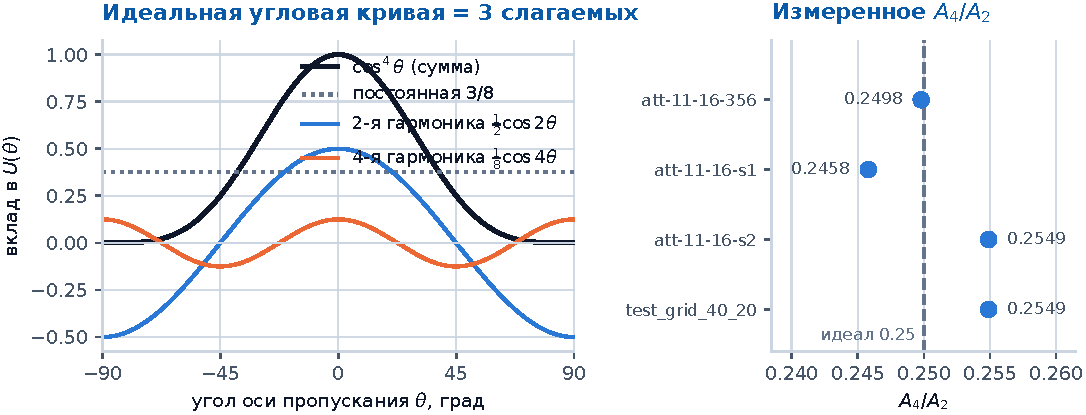
\includegraphics[width=\linewidth]{figures/fig00_harmonics.pdf}
  \caption{Слева: идеальная угловая кривая $\cos^4\theta$ раскладывается ровно на постоянную,
  вторую и четвёртую гармоники угла~--- это тождество, а не приближение. Справа: измеренное
  отношение амплитуд четвёртой и второй гармоник против идеального значения~$0.25$; отклонение
  менее~2\,\%. Числа перенесены из \artifact{BRIEF\_FOR\_D\_teaching\_ladder.md} §5.2.}
  \label{fig:harmonics}
\end{figure}

\paragraph{Цена вопроса~--- конкретное число.} Из-за перекрёстного члена угловая зависимость
$U(\theta)$ раскладывается по \emph{пяти} функциям
$\{1,\cos2\theta,\sin2\theta,\cos4\theta,\sin4\theta\}$, а не по трём, как было бы в некогерентном
(учебном) случае. Именно четвёртая гармоника несёт относительную фазу каналов, то есть~$\tleak$
из~\S\ref{subsec:phase}.

\begin{projectfact}[: разложение точно, а не приближённо]
Численная проверка на синтетике: невязка разложения $\mathrm{rms}=1.4\times10^{-16}$~--- машинный
ноль. \artifact{research/two\_wgp/NOTE\_malus\_linearization.md}, артефакт
\artifact{research/results/two\_wgp/a0\_malus\_linearization.json}.

Отношение амплитуд четвёртой и второй гармоник для идеального $\cos^4\theta$ равно ровно~$0.25$;
на данных~--- \texttt{356att} $0.2498$, \texttt{s1} $0.2458$, \texttt{s2} $0.2549$,
\texttt{test\_grid} $0.2549$ (рис.~\ref{fig:harmonics}). Игнорировать четвёртую гармонику~---
значит выбросить около четверти сигнала.
\end{projectfact}

\begin{tcolorbox}[enhanced,colback=cS1!7,colframe=cS1,boxrule=0pt,leftrule=3pt,arc=1pt]
\textbf{Мораль для всего курса.} Различение «поле против интенсивности»~--- не философия. Оно
решает, сколько независимых чисел содержит одно измерение: \textbf{пять, а не три}. А сколько чисел
содержит измерение~--- это, как выяснится в~\S5 и~\S9, и есть главный вопрос всего проекта:
параметров в модели может быть больше, чем измерение содержит независимых чисел.
\end{tcolorbox}

% ---------------------------------------------------------------------
\subsection{Поляризация и поворот осей}

\begin{intuition}
Волна бежит вдоль~$z$, поле колеблется поперёк~--- в плоскости $(x,y)$. \term{Поляризация} отвечает
на вопрос, по какой траектории в этой плоскости движется кончик вектора поля. Вдоль прямой~---
\emph{линейная} поляризация, и её достаточно задать одним углом.
\end{intuition}

\noindent
Поле под углом~$\alpha$ к оси~$x$ раскладывается на проекции, а переход между системами координат
выполняется обычной матрицей поворота:
\[
  \vec{E}=E_0\begin{pmatrix}\cos\alpha\\ \sin\alpha\end{pmatrix},
  \qquad
  \Rot{\theta}=\begin{pmatrix}\cos\theta & -\sin\theta\\[2pt] \sin\theta & \cos\theta\end{pmatrix}.
\]
Этого достаточно: физика элемента записывается в его \emph{собственных} осях, а в лабораторные
переводится сопряжением $\Rot{\theta}\,(\cdot)\,\Rot{-\theta}$. Подробный разбор с выводом закона
Малюса~--- \S1.

% ---------------------------------------------------------------------
\subsection{Решётка проводов как анизотропный лист}
\label{subsec:grid}

\begin{intuition}
Проволочный поляризатор~--- плоскость параллельных металлических проволок. Что произойдёт с волной,
зависит только от ориентации поля относительно проволок. Поле \emph{вдоль} проволок гонит электроны
вдоль проволоки, течёт ток, ток переизлучает волну назад~--- волна отражается. Поле \emph{поперёк}
проволок двигать электроны почти не может (поперёк проволока тонкая)~--- волна проходит.
\end{intuition}

\begin{figure}[t]
  \centering
  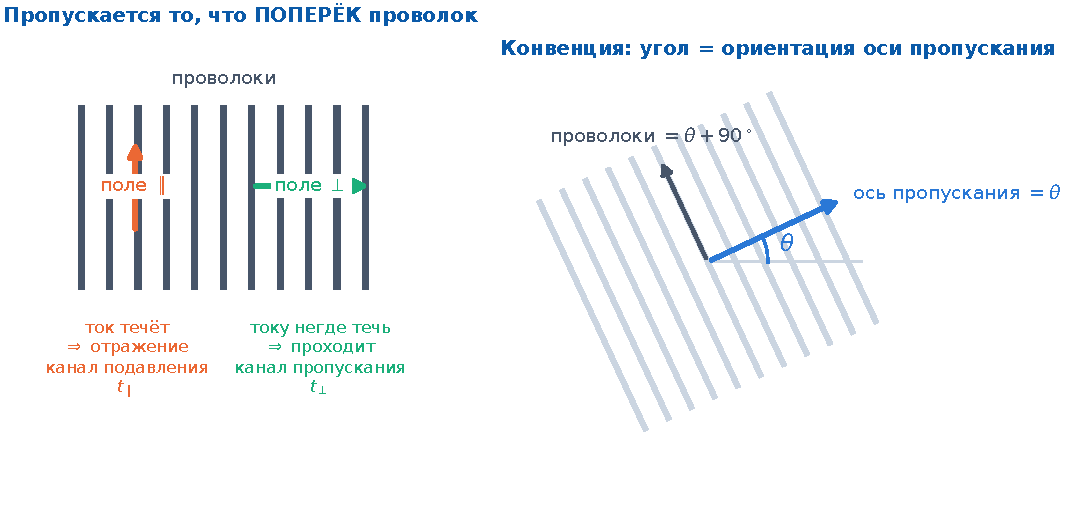
\includegraphics[width=\linewidth]{figures/fig00_geometry.pdf}
  \caption{Слева: два канала решётки. Справа: конвенция репозитория~--- угол элемента есть
  ориентация \emph{оси пропускания}, проволоки лежат под углом $\theta+90^\circ$
  (\artifact{research/two\_wgp/model\_2wgp.py}).}
  \label{fig:geometry}
\end{figure}

\needspace{8\baselineskip}   % не давать рисунку разорвать эту врезку
\begin{warning}[: здесь ошибаются почти все]
Проволочная решётка~--- \textbf{не щель}. Интуиция «щель в заборе пропускает то, что вдоль щели»
даёт \emph{противоположный} ответ. Правильно: \textbf{поляризатор пропускает поле, перпендикулярное
проволокам.} Ошибка стоит поворота всех углов на~$90^\circ$ и переворачивает физический смысл
каждого результата.
\end{warning}

\noindent
Отсюда \term{конвенция репозитория}: угол элемента~--- ориентация \emph{оси пропускания}
(перпендикуляра к проволокам), сами проволоки лежат под углом $+90^\circ$ к ней. Читая в проекте
«угол~$\theta$», подставляйте «ось пропускания», а не «проволоки».

\begin{strict}
В собственных осях решётки её действие~--- диагональная матрица
\[
  J_{\text{решётка}}=\begin{pmatrix}\tperp(\nu) & 0\\[2pt] 0 & \tpar(\nu)\end{pmatrix},
\]
то есть вся электродинамика решётки сводится к \emph{двум комплексным числам на каждой частоте}.
Откуда эти числа берутся аналитически~--- \S2 (модель Бланко); какие материальные поправки к ним
добавляются~--- \S3 (Друде и рассеяние~$\nu^\gamma$).
\end{strict}

% ---------------------------------------------------------------------
\subsection{Подволновой режим: почему решётка «сплошная»}

\paragraph{Вопрос.} Решётка~--- периодическая структура с промежутками. Почему она описывается
двумя числами, а не картиной дифракции на каждой проволоке?

\begin{intuition}[: ответ в соотношении масштабов]
Рабочий диапазон проекта $0.2\ldots1.5$~ТГц, период решёток $P=15\ldots40$~мкм, то есть
$\lambda=200\ldots1500$~мкм и $P/\lambda\lesssim0.2$. Волна на порядок-два длиннее периода и
физически не разрешает отдельные проволоки~--- так же, как длинная океанская волна не «видит»
отдельных свай пирса, а чувствует пирс целиком (рис.~\ref{fig:scales}).
\end{intuition}

\begin{figure}[t]
  \centering
  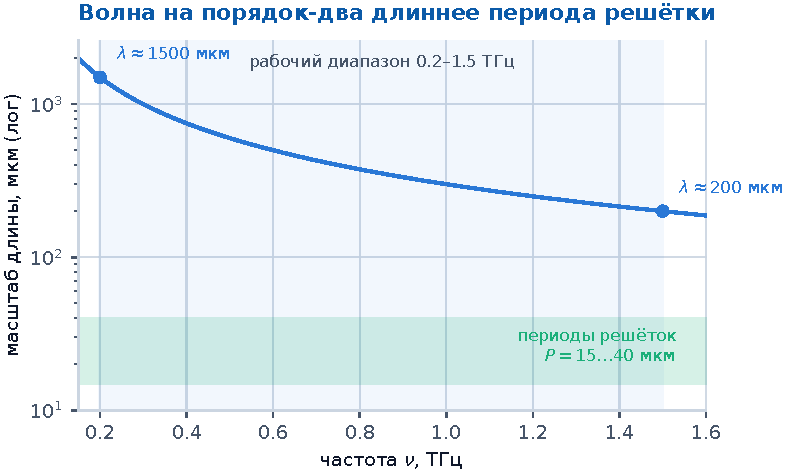
\includegraphics[width=0.78\linewidth]{figures/fig00_scales.pdf}
  \caption{Длина волны во всём рабочем диапазоне на порядок-два превышает период решёток проекта.
  Отсюда подволновой режим и законность описания решётки эффективным листом.}
  \label{fig:scales}
\end{figure}

\begin{strict}[: дифракционные порядки]
Решётка с периодом~$P$ рассеивает волну в порядки с поперечным волновым числом
$k_x^{(m)}=k\sin\alpha_{\text{пад}}+2\pi m/P$. Порядок распространяется, только если
$|k_x^{(m)}|\le k=2\pi/\lambda$, то есть требуется $P\gtrsim\lambda$. При $P\ll\lambda$ все порядки
$m\neq0$ имеют $|k_x^{(m)}|>k$, продольное волновое число $k_z=\sqrt{k^2-k_x^2}$ становится
\emph{мнимым}, и такие волны \term{эванесцентны}: экспоненциально затухают от решётки и энергию не
уносят.

\textbf{Следствие.} В дальнее поле уходит только нулевой порядок. Наблюдаемая~--- одно прошедшее
поле, а не набор пучков, и структура законно заменяется эффективным анизотропным листом с двумя
коэффициентами $\tperp,\tpar$. Именно это оправдывает весь формализм Джонса в проекте.
\end{strict}

\begin{projectfact}[: тот же объект в другом диапазоне~--- обычная решётка]
Период образца \texttt{purewave} независимо измерен по дифракции лазерной указки:
$P=23.4\pm0.8$~мкм~--- согласуется с микрофотографией $25.5\pm0.9$~мкм в пределах $1.8\sigma$
(Сессия~A, задача~A8; \artifact{coordination/BOARD.md}, запись от 2026-08-04).

Обратите внимание: дифракционные порядки \emph{видимого} света на этой решётке прекрасно
наблюдаются ($\lambda\approx0.65$~мкм $\ll P$). Подволновой режим~--- свойство не решётки, а
\emph{пары} «решётка~+~длина волны».
\end{projectfact}

% ---------------------------------------------------------------------
\subsection{Параметр плотности $D/P$}

\begin{intuition}
$D$~--- диаметр проволоки, $P$~--- период (расстояние между осями соседних проволок). Безразмерное
отношение $D/P$~--- доля периода, занятая металлом. В подволновом режиме абсолютные размеры сами по
себе не важны: важны их отношения к $\lambda$ и друг к другу. Именно $D/P$ управляет тем, насколько
плотно решётка «замыкает» тёмный канал.
\end{intuition}

\begin{figure}[t]
  \centering
  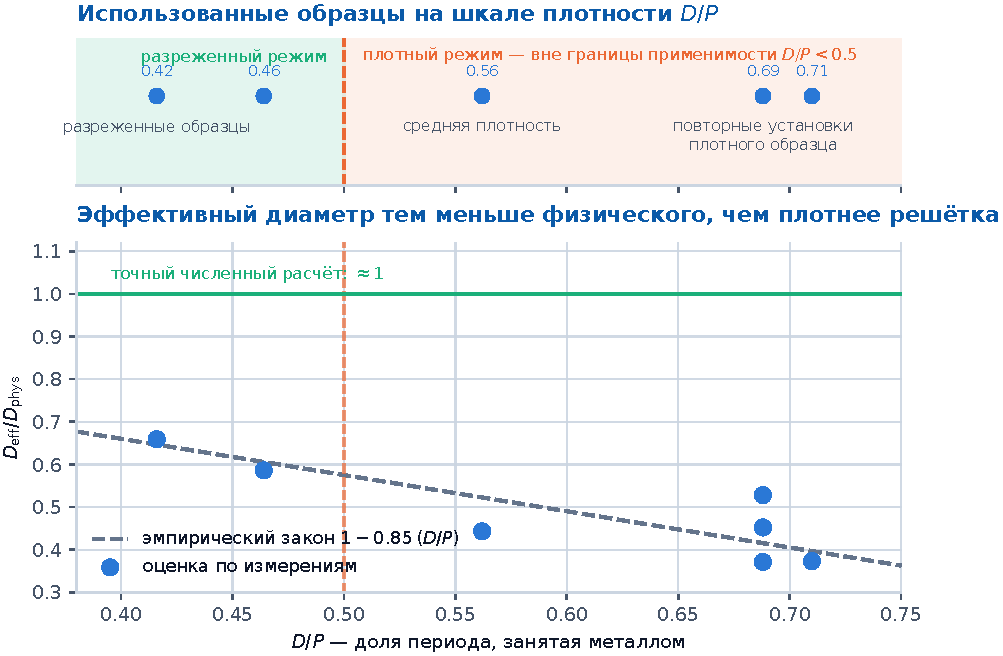
\includegraphics[width=0.86\linewidth]{figures/fig00_dp.pdf}
  \caption{Вверху: положение семи наборов проекта на шкале плотности и граница применимости
  аналитики, объявленная самим Бланко ($d/p<0.5$). Внизу: дефицит эффективного диаметра против
  плотности вместе с эмпирическим законом $1-0.85\,(D/P)$ и результатом точного расчёта. Числа~---
  \artifact{BRIEF\_FOR\_D\_teaching\_ladder.md} §11.3, колонка полного углового диапазона.}
  \label{fig:dp}
\end{figure}

\noindent
Практически все различия между образцами в проекте выстраиваются именно по $D/P$~--- не по
производителю и не по дате съёмки (рис.~\ref{fig:dp}):

\begin{itemize}[leftmargin=1.4em,itemsep=0.25em]
  \item \textbf{утечка тёмного канала:} $\eta\approx0.012$ при $D/P=0.71$ против $\approx0.033$ при
        $D/P=0.46$~--- более плотная решётка течёт \emph{слабее}, то есть является лучшим
        поляризатором (знак физически верен, \artifact{research/SYNTHESIS.md} §2);
  \item \textbf{применимость аналитики:} сам Бланко объявил границу $d/p<0.5$~--- плотные образцы
        проекта лежат \emph{вне} паспорта модели (находка Сессии~L,
        \artifact{research/papers/litrev/answers/}; подробно в~\S2);
  \item \textbf{дефицит эффективного диаметра} $\Deff/\Dphys$ монотонно падает от $0.659$ при
        $D/P=0.416$ до $0.373$ при $D/P=0.710$, тогда как точный расчёт даёт $\approx1$. Это
        центральная открытая загадка проекта, и разбирается она в~\S6 и~\S9.
\end{itemize}

\begin{warning}[: терминология, обязательная и в статье]
Четыре набора \texttt{att-11-16-*}~--- это \textbf{не четыре образца}, а ОДИН прибор
(ATT-11-16-CA85, S/N~\#02721) в четырёх условиях съёмки
(\artifact{BRIEF\_FOR\_D\_teaching\_ladder.md} §11.4). Называть их четырьмя образцами~--- значит
вчетверо завысить объём выборки.
\end{warning}

% ---------------------------------------------------------------------
\subsection{Честная оговорка: пучок конечной ширины}

Всё изложенное выше молча предполагало \term{плоскую волну}~--- бесконечно широкий фронт и один
угол падения. Реальный эксперимент устроен не так, и об этом следует сказать прямо (в статье это
идёт в раздел ограничений).

\begin{projectfact}[: сколько длин волн укладывается в пучок]
Пучок в перетяжке имеет диаметр $1.5\ldots2$~мм (\artifact{data\_pool/purewave/README.md}, раздел
про оптическую схему). При $\lambda=200\ldots1500$~мкм это всего \textbf{1--10 длин волн}.
\end{projectfact}

\noindent
Отсюда три следствия:
\begin{enumerate}[leftmargin=1.6em,itemsep=0.3em]
  \item \textbf{«Угол падения»~--- не одно число.} Сфокусированный пучок есть суперпозиция плоских
        волн с разными направлениями (широкий угловой спектр), тогда как аналитическая модель
        считает нормальное падение одной плоской волны.
  \item \textbf{Пространственное разрешение частотно-зависимо.} Низкие частоты «размазаны» шире
        высоких, то есть разные частоты опрашивают \emph{разные участки} образца.
  \item \textbf{Реальный кейс, стоивший проекту отозванного вывода.} Поляризатор в перетяжке был
        намеренно смещён относительно оси вращения. Узкий пучок при повороте образца описывает по
        апертуре окружность~--- следовательно, \emph{угол и участок образца перепутаны}. Вывод по
        гипотезе HN15 («дефицит $\Deff$ растёт с нерегулярностью решётки») был опубликован утром и
        отозван тем же вечером после уточнения схемы владельцем; текущий статус HN15~---
        \textbf{НЕ ПРОВЕРЕНА} (\artifact{BRIEF\_FOR\_D\_teaching\_ladder.md} §11.2).
\end{enumerate}

\begin{warning}[: правило, которое стоит запомнить раньше всей математики]
Прежде чем интерпретировать угловую развёртку, убедитесь, что образец отцентрован на оси вращения.
Иначе пространственная неоднородность образца подмешивается в $U(\theta)$~--- и, в отличие от
честной физики поляризатора, она \emph{не обязана быть чётной по}~$\theta$. Это, кстати,
действующий кандидат-объяснение асимметрии, отвергшей гипотезу~HN13 ($9.3\sigma$ / $4.2\sigma$;
не проверено).
\end{warning}

% ---------------------------------------------------------------------
\subsection{Типичные ошибки этого параграфа}

\begin{enumerate}[leftmargin=1.6em,itemsep=0.25em]
  \item Считать, что решётка пропускает поле \emph{вдоль} проволок. Наоборот
        (\S\ref{subsec:grid}).
  \item Путать угол оси пропускания с углом проволок. В коде проекта угол~--- ось пропускания.
  \item Переносить интенсивностную интуицию на THz-TDS. Детектор меряет \emph{поле}
        (\S\ref{subsec:field-vs-intensity}); отсюда пять, а не три независимых числа, и отсюда же
        вообще существует наблюдаемая~$\tleak$.
  \item Считать фазу технической деталью. Наклон фазы по частоте~--- это время
        (\S\ref{subsec:phase}), и оно измерено дважды независимо.
  \item Забывать про подволновость. Формализм $2\times2$ законен именно потому, что $P\ll\lambda$;
        на видимом свете тот же образец~--- обычная дифракционная решётка.
  \item Оперировать абсолютными микронами вместо~$D/P$: в подволновом режиме физику определяют
        безразмерные отношения.
  \item Молча предполагать плоскую волну. Пучок шириной 1--10 длин волн~--- это, помимо прочего,
        готовый механизм смешивания угла с координатой на образце.
\end{enumerate}

% ---------------------------------------------------------------------
\subsection*{Источники фактуры параграфа}
\addcontentsline{toc}{subsection}{\quad Источники фактуры §0}

\begin{center}
\footnotesize
\setlength{\tabcolsep}{4pt}
\begin{tabular}{@{}p{0.44\linewidth}>{\raggedright\arraybackslash}p{0.52\linewidth}@{}}
\toprule
\textbf{Утверждение} & \textbf{Артефакт} \\
\midrule
Данные~--- поле, не интенсивность & \texttt{CLAUDE.md} «Данные»; \texttt{data\_pool/**} \\
Пятимерный гармонический базис, невязка $1.4\times10^{-16}$ & \texttt{research/two\_wgp/NOTE\_malus\_linearization.md}; \texttt{results/two\_wgp/a0\_malus\_linearization.json} \\
$A_4/A_2$ по образцам ($0.2458\ldots0.2549$) & \texttt{BRIEF\_FOR\_D\_teaching\_ladder.md} §5.2 \\
$\tleak=0.19$~пс, сдвиг пика $-0.31$~пс & \texttt{research/SYNTHESIS.md} (HN8) \\
Конвенция угла = ось пропускания & \texttt{research/two\_wgp/model\_2wgp.py} \\
Период по дифракции $23.4\pm0.8$ против микрофото $25.5\pm0.9$~мкм & Сессия~A, A8; \texttt{coordination/BOARD.md} (2026-08-04) \\
Таблица $D/P$ и $\Deff/\Dphys$ по семи наборам & \texttt{BRIEF\_FOR\_D\_teaching\_ladder.md} §11.3 \\
Граница применимости Бланко $d/p<0.5$ & \texttt{research/papers/litrev/answers/} (Сессия~L, P1) \\
Пучок 1.5--2~мм, смешивание угла с участком, статус HN15 & \texttt{data\_pool/purewave/README.md}; \texttt{BRIEF\_FOR\_D\_teaching\_ladder.md} §11.2 \\
\bottomrule
\end{tabular}
\end{center}

\clearpage
      % §0  Электродинамика: необходимый минимум          [ГОТОВ]
% =====================================================================
%  §1. Матрицы Джонса: язык поляризационной оптики
%
%  ЖАНР (STYLE.md): учебная литература. Ни путей, ни имён программ, ни
%  номеров гипотез. Прослеживаемость — ключи \srckey{1.x} и приложение.
%
%  Содержательная основа: primers/01_jones_polarization.md (markdown
%  первичен по фактуре, LaTeX — по подаче).
% =====================================================================
\section{Матрицы Джонса: язык поляризационной оптики}
\label{sec:jones}
\markboth{§\thesection. Матрицы Джонса}{}

В §\ref{sec:electrodynamics} решётка проводов свелась к двум комплексным числам на каждой частоте.
Теперь нужен аппарат, который позволит собрать из таких элементов \emph{установку} и получить
формулу для измеряемой величины. Этот аппарат~--- матрицы Джонса~--- занимает полстраницы, а
работает весь курс: именно из него получается угловая зависимость $U(\theta)$, которую мы будем
подгонять в Части~II.

Ближе к концу параграфа мы применим его к содержательному вопросу: наша установка содержит
\emph{два} неидеальных поляризатора, а модель учитывает неидеальность только одного. Оказывается,
можно доказать~--- на бумаге, до всяких вычислений,~--- что второй ничего не изменит.

\begin{tcolorbox}[enhanced,colback=cPanel,colframe=cGrid,boxrule=0.8pt,arc=2pt,
                  title={\bfseries\color{cAccent} Пререквизиты},coltitle=cAccent,
                  attach boxed title to top left={xshift=6pt,yshift=-2pt},
                  boxed title style={colback=cPanel,boxrule=0pt,arc=0pt},top=10pt]
\textbf{Нужно знать:} §\ref{sec:electrodynamics} (комплексная амплитуда, поле против
интенсивности, два канала решётки); умножение матрицы $2\times2$ на вектор; матрица
поворота.\\[0.3em]
\textbf{Знать НЕ нужно:} теорию когерентности, матрицы Мюллера, формализм вектора Стокса. Где
проходит граница применимости и когда нужен более общий аппарат~--- сказано в §\ref{subsec:limits}.
\end{tcolorbox}

% ---------------------------------------------------------------------
\subsection{Вектор Джонса: состояние поляризации как два числа}

\begin{intuition}
Волна бежит вдоль~$z$, поле колеблется в плоскости $(x,y)$. Чтобы полностью описать колебание,
достаточно сказать, что происходит с проекцией на~$x$ и с проекцией на~$y$: у каждой своя
амплитуда и своя фаза. Итого четыре вещественных числа, или~--- что то же самое~--- два
комплексных.
\end{intuition}

\noindent
\term{Вектор Джонса}~--- столбец из двух комплексных амплитуд:
\[
  \mathbf{E}=\begin{pmatrix}\Efield_x\\[2pt] \Efield_y\end{pmatrix}\in\mathbb{C}^2 .
\]
Несколько состояний, полезных как ориентиры:
\[
  \begin{pmatrix}1\\0\end{pmatrix}\ \text{--- линейная вдоль }x,
  \qquad
  \begin{pmatrix}0\\1\end{pmatrix}\ \text{--- линейная вдоль }y,
\]
\[
  \frac{1}{\sqrt2}\begin{pmatrix}1\\1\end{pmatrix}\ \text{--- линейная под }45^\circ,
  \qquad
  \frac{1}{\sqrt2}\begin{pmatrix}1\\ \jj\end{pmatrix}\ \text{--- круговая.}
\]

\begin{intuition}[: откуда в круговой поляризации берётся $\jj$]
Множитель~$\jj$ означает сдвиг фазы на четверть периода. Пока проекция на~$x$ проходит максимум,
проекция на~$y$ проходит ноль~--- и наоборот. Кончик вектора поля не может при этом двигаться по
прямой: он описывает окружность. Вся «круговость» состоит из одного множителя.
\end{intuition}

% ---------------------------------------------------------------------
\subsection{Матрица Джонса и правило каскада}

\begin{strict}
Любой линейный оптический элемент, не меняющий частоту и не разрушающий поляризацию, действует на
вектор Джонса умножением на матрицу $2\times2$ с комплексными элементами:
\[
  \mathbf{E}_{\text{вых}}=\mathbf{J}\,\mathbf{E}_{\text{вх}},
  \qquad \mathbf{J}\in\mathbb{C}^{2\times2}.
\]
\end{strict}

\noindent
Три свойства, которыми мы будем пользоваться постоянно.

\paragraph{1. Линейность.} Она не постулируется ради удобства, а следует из линейности уравнений
Максвелла в среде без нелинейного отклика. Поля терагерцового импульса для этого более чем
слабы.

\paragraph{2. Каскад есть произведение~--- справа налево.} Если свет прошёл сначала элемент
$\mathbf{J}_1$, затем $\mathbf{J}_2$, то
\[
  \mathbf{E}_{\text{вых}}=\mathbf{J}_2\,\mathbf{J}_1\,\mathbf{E}_{\text{вх}} .
\]
Порядок сомножителей обратен порядку прохождения, и переставлять их нельзя: матрицы не
коммутируют. Это не формальность~--- два поляризатора, поставленные в разном порядке, дают разный
результат, что легко проверить и на оптическом столе.

\paragraph{3. Поворот элемента~--- сопряжение матрицей поворота.} Физика элемента проста в
\emph{его собственных} осях. Чтобы применить её к полю, заданному в лабораторной системе, поле
переводят в оси элемента, действуют, и результат переводят обратно:
\begin{equation}
  \mathbf{J}(\theta)=\Rot{\theta}\,\mathbf{J}_{\text{собств}}\,\Rot{-\theta},
  \qquad
  \Rot{\theta}=\begin{pmatrix}\cos\theta & -\sin\theta\\[2pt] \sin\theta & \cos\theta\end{pmatrix}.
  \label{eq:rotation}
\end{equation}

\begin{intuition}[: почему «туда и обратно», а не просто умножение на $\Rot{\theta}$]
Матрица элемента знает только слова «вдоль проволок» и «поперёк проволок». Поле, записанное в
лабораторных осях, для неё~--- на чужом языке. Поэтому его сначала переводят
($\Rot{-\theta}$), затем элемент действует, и ответ переводят обратно ($\Rot{\theta}$). Это
стандартная смена базиса $\mathbf{J}_{\text{лаб}}=\mathbf{R}\,\mathbf{J}_{\text{собств}}
\mathbf{R}^{-1}$, а для поворота $\mathbf{R}^{-1}=\Rot{-\theta}$.
\end{intuition}

% ---------------------------------------------------------------------
\subsection{Идеальный поляризатор и закон Малюса}
\label{subsec:malus}

Идеальный поляризатор с осью пропускания вдоль~$x$ пропускает $x$-компоненту целиком и уничтожает
$y$-компоненту:
\[
  \mathbf{J}_{\text{ид}}=\begin{pmatrix}1&0\\0&0\end{pmatrix},
  \qquad
  \mathbf{J}_{\text{ид}}\begin{pmatrix}a\\b\end{pmatrix}=\begin{pmatrix}a\\0\end{pmatrix}.
\]
Это \term{проектор}: применённый дважды, он даёт то же, что и один раз.

\paragraph{Классический закон Малюса.} Два идеальных поляризатора, второй повёрнут на~$\theta$
относительно первого. Прошедшая амплитуда $\propto\cos\theta$, интенсивность
$\propto\cos^2\theta$; при $\theta=90^\circ$ (скрещённые поляризаторы)~--- ноль.

\begin{warning}[: в нашей схеме показатель степени другой]
Схема измерения содержит \emph{три} поляризационных элемента: поляризатор, задающий вход,
исследуемый образец под углом~$\theta$ и анализатор перед приёмником
(рис.~\ref{fig:cascade}). Косинус набегает \textbf{дважды}: один раз при проекции входного поля
на ось образца, второй раз при проекции прошедшего поля на ось анализатора. Поэтому
\[
  \Efield(\theta)\propto\cos^2\theta
  \quad\text{по амплитуде},
  \qquad
  U(\theta)\propto\cos^4\theta
  \quad\text{по энергии,}
\]
а не $\cos^2\theta$, как в учебниковой формулировке закона Малюса. Ожидание «должно быть
$\cos^2$» приводит к систематическому расхождению модели и данных~--- и к соблазну объяснить его
физикой, которой нет.
\end{warning}

\begin{figure}[t]
  \centering
  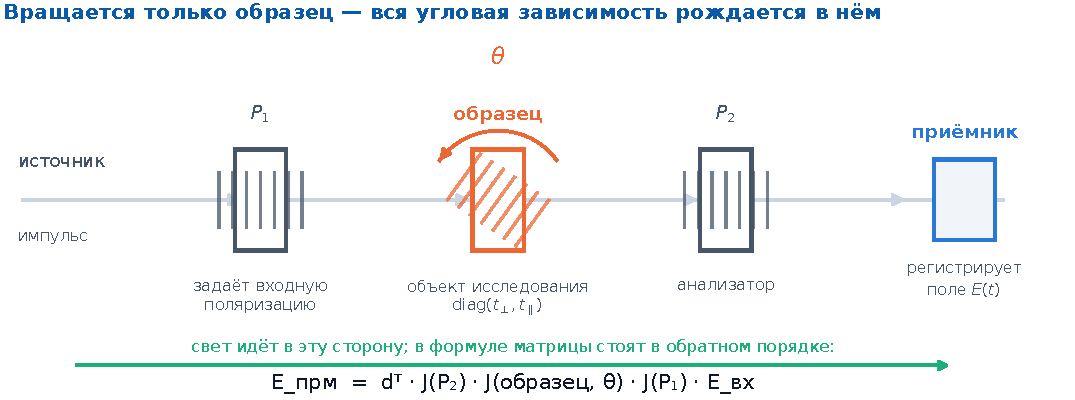
\includegraphics[width=\linewidth]{figures/fig01_cascade.pdf}
  \caption{Схема измерения на языке матриц Джонса; штриховка внутри элементов показывает
  направление проволок. Свет проходит элементы слева направо, а матрицы в формуле стоят в
  обратном порядке. Вращается только исследуемый образец; остальные элементы неподвижны, поэтому
  вся угловая зависимость наблюдаемой рождается в нём.}
  \label{fig:cascade}
\end{figure}

\begin{strict}[: вывод угловой зависимости]
Пусть вход поляризован вдоль~$x$, анализатор и приёмник тоже настроены на~$x$, а образец с
матрицей $\mathrm{diag}(\tperp,\tpar)$ повёрнут на~$\theta$. Подставляя~\eqref{eq:rotation} и
беря $x$-компоненту результата, получаем
\begin{equation}
  \Efield(\theta)=\tperp\cos^2\theta+\tpar\sin^2\theta .
  \label{eq:malus-jones}
\end{equation}
Это то самое выражение, которое в §\ref{sec:electrodynamics} было принято без вывода. При
$\tperp=1$, $\tpar=0$ оно даёт $\cos^2\theta$ по амплитуде, то есть $\cos^4\theta$ по энергии.
\end{strict}

\begin{intuition}[: как читать формулу~\eqref{eq:malus-jones}]
Два слагаемых~--- два пути, по которым поле попадает на приёмник. Первый: поле прошло через канал
пропускания образца, и его вклад ослаблен геометрической проекцией $\cos^2\theta$. Второй: поле
прошло через канал подавления, где образец обязан был его погасить, и вклад взвешен
$\sin^2\theta$. Вблизи $\theta=90^\circ$ первый путь закрыт геометрией, и на приёмник приходит
почти исключительно то, что \emph{просочилось}. Именно поэтому область глубокого подавления~---
самая информативная часть развёртки.
\end{intuition}

% ---------------------------------------------------------------------
\subsection{Реальный поляризатор: просачивание и его фаза}
\label{subsec:leakage}

Вынесем за скобку пропускание рабочего канала:
\begin{equation}
  \begin{pmatrix}\tperp&0\\0&\tpar\end{pmatrix}
  =\tperp\begin{pmatrix}1&0\\[2pt]0&\eta\,e^{\jj\delta}\end{pmatrix},
  \qquad
  \eta=\left|\frac{\tpar}{\tperp}\right|,
  \quad
  \delta=\arg\frac{\tpar}{\tperp}.
  \label{eq:leaky}
\end{equation}

Такая запись отделяет общий множитель (насколько прибор ослабляет свет вообще) от того, что нас
интересует: насколько плохо он подавляет ненужную поляризацию. Появились две содержательные
величины.

\begin{itemize}[leftmargin=1.4em,itemsep=0.35em]
  \item $\eta$~--- \term{просачивание}: доля \emph{амплитуды}, проходящая там, где должен быть
        ноль.
  \item $\delta$~--- \term{фаза просачивания}: насколько просочившееся поле запаздывает
        относительно прошедшего. В §\ref{sec:electrodynamics} мы видели, что линейная по частоте
        фаза есть временная задержка; поэтому осмысленная параметризация~---
        $\delta(\nu)=\delta_0+2\pi\nu\,\tleak$.
\end{itemize}

\begin{warning}[: амплитуда и мощность~--- не одно и то же]
\term{Коэффициент экстинкции} принято выражать через мощность:
\[
  \mathrm{ER}=\frac{1}{\eta^{2}},
  \qquad
  \mathrm{ER}\,[\text{дБ}]=-20\log_{10}\eta .
\]
Отсюда обычная ошибка на множитель два в децибелах: часть литературы (и, в частности,
аналитическая модель, к которой мы перейдём в §2) публикует коэффициенты \emph{по мощности}
$|\tperp|^2$ и $|\tpar|^2$, тогда как в матрицах Джонса стоят \emph{амплитудные}~$\tperp,\tpar$.
Забытый квадрат искажает результат ровно вдвое по шкале децибел.
\end{warning}

\begin{example}[: насколько хорош реальный поляризатор]\srckey{1.1}
На семи наборах измерений относительная амплитуда просачивания составила
\[
  \eta\approx0{,}012\ldots0{,}036,
\]
что отвечает коэффициенту экстинкции примерно от $29$ до $38$~дБ. Меньшие значения~--- у плотных
решёток, большие~--- у разреженных: связь с $D/P$ обсуждалась в §\ref{sec:electrodynamics}.

Для сравнения: плёночные поляризаторы, используемые в схеме как эталонные, дают лучше $39$~дБ~---
в терагерцовом диапазоне их можно считать идеальными проекторами.
\end{example}

\begin{figure}[t]
  \centering
  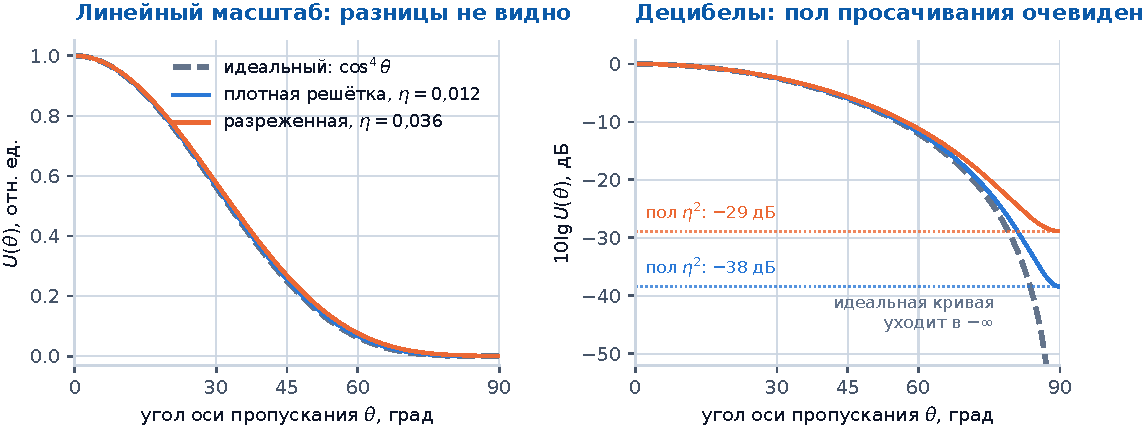
\includegraphics[width=\linewidth]{figures/fig01_malus_floor.pdf}
  \caption{Модельный расчёт по формуле~\eqref{eq:malus-jones} с реалистичными значениями
  просачивания. Слева, в линейном масштабе, идеальная и реальная кривые неразличимы. Справа, в
  децибелах, различие очевидно: вместо нуля при $90^\circ$ кривая упирается в \emph{пол}
  просачивания на уровне $\eta^2$. Уровень пола и есть измеряемая величина.}
  \label{fig:floor}
\end{figure}

\begin{intuition}[: почему просачивание видно только в логарифмическом масштабе]
Величина $\eta^2\sim10^{-3}$ на фоне единицы~--- одна тысячная. В линейном масштабе такая добавка
не видна глазом и почти не влияет на сумму квадратов невязок: подгонка её попросту не заметит.
В децибелах та же добавка~--- это разница между «минус бесконечность» и «минус тридцать»,
то есть между нулём и вполне уверенно измеримым сигналом.

Отсюда практическое правило, к которому мы вернёмся в §7 при обсуждении весов: \textbf{шкала, в
которой вы смотрите на данные, определяет, какие параметры вы способны измерить.}
\end{intuition}

% ---------------------------------------------------------------------
\subsection{Полная установка: где живут неидеальности}
\label{subsec:full-chain}

Запишем весь тракт. Свет проходит поляризатор~$P_1$, исследуемый образец под углом~$\theta$,
анализатор~$P_2$ и попадает на приёмник, чувствительный к одной линейной компоненте (вектор
чувствительности~$\mathbf{d}$):
\begin{equation}
  \Efield_{\text{прм}}
  =\mathbf{d}^{\mathsf T}\,\mathbf{J}_{P_2}\,\mathbf{J}_{\text{обр}}(\theta)\,
   \mathbf{J}_{P_1}\,\mathbf{E}_{\text{вх}} .
  \label{eq:chain}
\end{equation}

Идеализация~\eqref{eq:malus-jones} предполагала, что всё, кроме образца, идеально. В
действительности неидеален каждый сомножитель:

\begin{center}
\footnotesize
\setlength{\tabcolsep}{6pt}
\begin{tabular}{@{}p{0.17\linewidth}p{0.33\linewidth}>{\raggedright\arraybackslash}p{0.44\linewidth}@{}}
\toprule
\textbf{Элемент} & \textbf{Роль} & \textbf{Чем неидеален} \\
\midrule
$\mathbf{J}_{P_1}$ & задаёт входную поляризацию & собственное просачивание \\
$\mathbf{J}_{\text{обр}}(\theta)$ & \textbf{объект исследования} & здесь живут $\tperp$, $\tpar$
и через них~--- геометрия решётки \\
$\mathbf{J}_{P_2}$ & анализатор & собственное просачивание; ось может быть развёрнута
относительно приёмника \\
$\mathbf{d}$ & приёмник & чувствительность к «неправильной» компоненте (кросс-поляризация) \\
\bottomrule
\end{tabular}
\end{center}

\begin{warning}[: центральная методическая трудность всей задачи]
Малый сигнал, наблюдаемый в скрещённом положении, может родиться в трёх разных местах:
просачивание образца, просачивание анализатора, кросс-поляризация приёмника. \emph{По величине
сигнала на~$90^\circ$ они неразличимы принципиально}~--- складываются в одно число.

Различать их приходится по \term{угловой сигнатуре}: просачивание образца зависит от угла (входит
с весом $\sin^2\theta$), а аппаратные вклады от поворота образца не зависят вовсе. Это работает,
но лишь отчасти: сигнатуры недостаточно различны.
\end{warning}

\begin{example}[: насколько удалось разделить]\srckey{1.2}
Оценки просачивания образца и кросс-поляризации приёмника в совместной подгонке коррелируют с
коэффициентом~$0{,}73$. Разделение получено \emph{частичное}, и в выводах это указано как
ограничение метода, а не как результат.

Число $0{,}73$ стоит запомнить: в §5 мы научимся вычислять такие корреляции заранее, до
подгонки, из одного лишь плана эксперимента, а в §9~--- отличать «плохо разделено» от «не
разделено в принципе».
\end{example}

% ---------------------------------------------------------------------
\subsection{Усложнение, которое можно отвергнуть до вычислений}
\label{subsec:alignment}

Схема~\eqref{eq:chain} ставит естественный вопрос. Модель считает анализатор идеальным, а он
реален~--- у него своё просачивание. Не в нём ли причина того, что модель требует странно
малого эффективного диаметра (§\ref{sec:electrodynamics})? Соблазн очевиден: усложнить модель,
добавив второй реальный поляризатор, и посмотреть, что скажет подгонка.

Прежде чем усложнять, полезно посчитать на бумаге.

\begin{strict}[: теорема о выровненном анализаторе]
\emph{Если ось пропускания анализатора совпадает с осью чувствительности приёмника, то реальный
анализатор тождественно эквивалентен идеальному, умноженному на скаляр $t_{\perp,2}(\nu)$.}

\smallskip
\textbf{Доказательство.} Пусть обе оси направлены по~$x$, тогда $\mathbf{d}^{\mathsf T}=(1,0)$ и
\[
  \mathbf{d}^{\mathsf T}\mathbf{J}_{P_2}
  =(1,0)\begin{pmatrix}t_{\perp,2}&0\\[2pt]0&t_{\parallel,2}\end{pmatrix}
  =(t_{\perp,2},\,0)
  =t_{\perp,2}\,\mathbf{d}^{\mathsf T}.
\]
Вся информация о неидеальности анализатора содержится в $t_{\parallel,2}$, а он умножается на
нулевую компоненту вектора чувствительности и в наблюдаемую не входит. $\square$
\end{strict}

\begin{intuition}[: что именно доказано]
Неидеальность анализатора не «мала» и не «пренебрежима»~--- она \emph{ненаблюдаема}. Приёмник
физически не может отличить реальный выровненный анализатор от идеального: единственный след,
который остаётся,~--- общий множитель $t_{\perp,2}(\nu)$, одинаковый для всех углов.

А раз множитель не зависит от~$\theta$, он не способен изменить \emph{форму} угловой
зависимости. Все параметры, извлекаемые из формы~--- а это, в частности, эффективный диаметр,~---
обязаны остаться прежними.
\end{intuition}

\begin{example}[: предсказание, сделанное до расчёта, и его проверка]\srckey{1.3}
Из теоремы следовало конкретное численное предсказание: явное включение второго реального
поляризатора в модель не улучшит согласия с данными и не сдвинет оценку эффективного диаметра.
Проверка на измерениях:

\begin{itemize}[leftmargin=1.4em,itemsep=0.2em]
  \item изменение информационного критерия $\dAIC=+0{,}15$~--- усложнённая модель не лучше
        исходной (шкала $\Delta$AIC разбирается в §8; здесь достаточно знать, что это «ничего не
        изменилось»);
  \item оценка эффективного диаметра: $4{,}694$~мкм до усложнения и $4{,}694$~мкм после~---
        совпадение в четырёх значащих цифрах.
\end{itemize}

Модель усложнили честно, и она отказалась усложняться ровно так, как было предсказано на бумаге.
\end{example}

\begin{tcolorbox}[enhanced,colback=cS1!7,colframe=cS1,boxrule=0pt,leftrule=3pt,arc=1pt]
\textbf{Мораль для метода.} Прежде чем усложнять модель и запускать подгонку, проверьте, не
сводится ли усложнение к общему множителю, не зависящему от переменной, по которой идёт
развёртка. Если сводится~--- подгонка заведомо ничего не покажет, и это известно заранее и
бесплатно. Такие «теоремы редукции» экономят недели вычислений и, что важнее, избавляют от
соблазна истолковать шум как эффект.
\end{tcolorbox}

\begin{warning}[: условие теоремы существенно]
Требуется именно \emph{выравнивание} осей анализатора и приёмника. Если они развёрнуты на
угол~$\phi_2$, произведение $\mathbf{d}^{\mathsf T}\mathbf{J}_{P_2}$ перестаёт быть
пропорциональным $\mathbf{d}^{\mathsf T}$, просачивание анализатора становится наблюдаемым и
подмешивается к просачиванию образца. Теорема~--- не разрешение не думать об анализаторе, а
указание, что именно нужно контролировать в юстировке.
\end{warning}

% ---------------------------------------------------------------------
\subsection{Границы применимости формализма}
\label{subsec:limits}

\begin{strict}
Матрицы Джонса описывают \textbf{полностью поляризованный когерентный} свет. Для частично
поляризованного или частично когерентного излучения двух комплексных амплитуд недостаточно:
нужен более общий аппарат~--- вектор Стокса и матрицы Мюллера ($4\times4$, действуют на
интенсивности, а не на поля).
\end{strict}

\noindent
В нашем случае формализм Джонса законен, и по вполне конкретной причине: приёмник регистрирует
поле когерентно (§\ref{sec:electrodynamics}), то есть измеряет амплитуду и фазу, а не усреднённую
мощность. Это то же самое свойство установки, из-за которого угловая зависимость содержит пять
независимых чисел, а не три.

\begin{intuition}[: связь двух утверждений]
Одно физическое обстоятельство~--- когерентная регистрация поля~--- даёт сразу две вещи:
законность матриц Джонса и наличие перекрёстного члена в наблюдаемой. Если бы приёмник мерил
интенсивность, пришлось бы перейти к матрицам Мюллера, и вместе с фазой исчезла бы часть
информации~--- в частности, задержка просачивания.
\end{intuition}

% ---------------------------------------------------------------------
\subsection{Типичные ошибки этого параграфа}

\begin{enumerate}[leftmargin=1.6em,itemsep=0.25em]
  \item Переставить сомножители в каскаде. Свет идёт слева направо, матрицы перемножаются справа
        налево: $\mathbf{J}_2\mathbf{J}_1\neq\mathbf{J}_1\mathbf{J}_2$.
  \item Ожидать $\cos^2\theta$ вместо $\cos^4\theta$. В схеме с анализатором проекция происходит
        дважды (§\ref{subsec:malus}).
  \item Спутать амплитудные коэффициенты с коэффициентами по мощности. Множитель два в
        децибелах~--- самая живучая ошибка в этой области.
  \item Отождествить просачивание и коэффициент экстинкции: $\mathrm{ER}=1/\eta^2$, это разные
        величины и разные шкалы.
  \item Отбросить фазу коэффициентов, оставив модули. Вместе с фазой теряется задержка
        просачивания~--- ровно то, ради чего ставился когерентный эксперимент.
  \item Применить матрицы Джонса к частично поляризованному свету (§\ref{subsec:limits}).
  \item Считать, что малый сигнал в скрещённом положении заведомо принадлежит образцу. У него
        три возможных источника, и разделяются они только по угловой зависимости
        (§\ref{subsec:full-chain}).
\end{enumerate}

\clearpage
                % §1  Матрицы Джонса: язык поляризационной оптики    [ГОТОВ]
% =====================================================================
%  §2. Модель Бланко: эквивалентная схема решётки проводов
%
%  ЖАНР (STYLE.md): учебная литература. Ни путей, ни имён программ, ни
%  номеров гипотез. Прослеживаемость — ключи \srckey{2.x} и приложение.
%
%  Содержательная основа: Blanco A., Fonti S., Piacente A. Transmission
%  coefficients of free-standing wire grids in the far infrared: a
%  theoretical approach for easy computation // Infrared Physics. 1986.
%  Vol. 26, no. 6. P. 357-363. DOI 10.1016/0020-0891(86)90058-8
%  (библиографическая сверка выполнена другой сессией, ключ 2.1).
% =====================================================================
\section{Модель Бланко: эквивалентная схема решётки проводов}
\label{sec:blanco}
\markboth{§\thesection. Модель Бланко}{}

В §\ref{sec:electrodynamics} решётка проводов была принята как данность: сплошной анизотропный
лист, задаваемый двумя комплексными числами $\tperp(\nu)$, $\tpar(\nu)$ на каждой частоте. В
§\ref{sec:jones} эти два числа заняли своё место в матрице элемента и дали угловую зависимость
$U(\theta)$. Оставался открытым главный вопрос: \emph{откуда берутся сами $\tperp$ и $\tpar$}, если
считать не эффективный лист, а настоящую решётку из круглых проводов с диаметром~$D$ и
периодом~$P$? Ответ~--- предмет этого параграфа, и он же задаёт первую жёсткую границу
применимости, с которой предстоит работать всему дальнейшему изложению.

\begin{tcolorbox}[enhanced,colback=cPanel,colframe=cGrid,boxrule=0.8pt,arc=2pt,
                  title={\bfseries\color{cAccent} Пререквизиты},coltitle=cAccent,
                  attach boxed title to top left={xshift=6pt,yshift=-2pt},
                  boxed title style={colback=cPanel,boxrule=0pt,arc=0pt},top=10pt]
\textbf{Нужно знать:} §\ref{sec:electrodynamics} (подволновой режим $P/\lambda\lesssim0{,}2$,
эванесцентность высших дифракционных порядков, параметр плотности $D/P$); понятие комплексного
сопротивления (импеданса) двухполюсника; последовательное и параллельное соединение элементов
цепи.\\[0.3em]
\textbf{Знать НЕ нужно:} строгую теорию дифракции на периодических структурах (ряды
Рэлея--Флоке, интегральные уравнения на профиле провода). Результат этой теории пересказывается
здесь в готовом виде~--- в форме, которую предложили сами авторы модели.
\end{tcolorbox}

% ---------------------------------------------------------------------
\subsection{От дифракционной задачи к электрической цепи}
\label{subsec:circuit-idea}

\begin{intuition}
Строгая электродинамическая задача~--- рассеяние волны на бесконечной решётке проводов~--- в общем
случае очень сложна: нужно решать интегральное уравнение на поверхности каждого провода. Но в
подволновом режиме ($P/\lambda\lesssim0{,}2$, §\ref{sec:electrodynamics}) распространяется только
нулевой дифракционный порядок, а все остальные экспоненциально затухают в первые же доли длины
волны от решётки. Это резко упрощает задачу: решётку можно заменить \emph{чёрным ящиком},
характеризуемым всего двумя числами на входе и выходе~--- ровно так же, как в электротехнике
сложную цепь заменяют одним эквивалентным сопротивлением, если интересует только то, что видно
снаружи.
\end{intuition}

\begin{strict}[: почему замена вообще законна]
Периодическая структура с периодом $P<\lambda$ поддерживает единственную распространяющуюся волну
по обе стороны от решётки~--- саму падающую/прошедшую плоскую волну. Вся информация о микроскопической
геометрии проводов (их форма, толщина, взаимное расположение) содержится в ближнем поле,
затухающем на масштабе~$P$, и на измеряемую волну влияет только через то, как решётка
\emph{в целом} связывает амплитуды по разные стороны. Такая связь по построению линейна и потому
эквивалентна двухпортовой электрической цепи: паре чисел (пропускание, отражение), которые можно
получить из импеданса эквивалентной схемы так же, как в теории длинных линий.
\end{strict}

\begin{intuition}[: связь с волноводной техникой]
Ровно тот же приём~--- заменять препятствие в волноводе (диафрагму, штырь, стык) эквивалентной
$LC$-цепью~--- давно применялся в микроволновой технике для расчёта волноводных фильтров:
классическое изложение~--- справочник Марковица (Marcuvitz, \emph{Waveguide Handbook}, 1951). Модель,
которую мы используем, распространяет этот приём со стенок волновода на свободное пространство:
решётка проводов рассматривается как периодическое препятствие в свободно распространяющейся
волне, а не в волноводе. Дальше в этом параграфе~--- лишь конкретизация того, какая именно схема
отвечает решётке проводов, и как её элементы выражаются через $D$, $P$ и~$\lambda$.
\end{intuition}

% ---------------------------------------------------------------------
\subsection{Два канала~--- две разные схемы}
\label{subsec:two-circuits}

Ключевое наблюдение: у решётки \emph{два} принципиально разных электрических портрета в
зависимости от того, вдоль проводов или поперёк них направлено поле,~--- то же деление на канал
пропускания и канал подавления, что и в §\ref{sec:electrodynamics}.

\begin{intuition}
Поле, направленное \textbf{вдоль проводов} (канал подавления, $\tpar$), видит почти сплошной
проводящий барьер: заряды в проводе свободно текут вдоль него и экранируют поле, решётка ведёт
себя как почти сплошное зеркало. В электрической аналогии барьер, который \emph{в основном
отражает}, соответствует \term{индуктивному шунту}~--- малому сопротивлению для проходящей волны.

Поле, направленное \textbf{поперёк проводов} (канал пропускания, $\tperp$), не может течь через
узкие промежутки между проводами так же свободно: провода воспринимаются как редкие препятствия в
почти пустом пространстве. Решётка в основном \emph{пропускает}, что в электрической аналогии
отвечает \term{ёмкостному шунту}~--- малому возмущению для проходящей волны.
\end{intuition}

Это ровно та анизотропия, которая в §\ref{sec:electrodynamics} была принята как факт (решётка~---
анизотропный лист): здесь видно её электрическое происхождение. Дальше нужно превратить эту
качественную картину в числа.

% ---------------------------------------------------------------------
\subsection{Геометрия входит через два безразмерных числа}
\label{subsec:A1A2}

Оба канала строятся из одного и того же строительного материала~--- пары безразмерных функций
$A_1$ и $A_2$, зависящих от отношения диаметра к периоду $D/P$ и периода к длине волны
$P/\lambda$:

\begin{equation}
  A_1=1+\tfrac12(\pi\tfrac{D}{\lambda})^2\Big[\ln\tfrac{1}{\pi D/P}+\tfrac34\Big]
        +\tfrac12(\pi\tfrac{D}{\lambda})^2\sum_{m=1}^{N}\Big(\tfrac1{C_m}-\tfrac1m\Big),
  \label{eq:A1}
\end{equation}
\begin{equation}
  A_2=1+\tfrac12(\pi\tfrac{D}{\lambda})^2\Big[\tfrac{11}{4}-\ln\tfrac{1}{\pi D/P}\Big]
        +\tfrac1{24}(\pi\tfrac{D}{\lambda})^2
        -(\pi\tfrac{D}{\lambda})^2\sum_{m=1}^{N}\Big(m-\tfrac1{2m}(\tfrac{P}{\lambda})^2-C_m\Big),
  \label{eq:A2}
\end{equation}
где $C_m=\sqrt{m^2-(P/\lambda)^2}$, а сумма по $m$ на практике сходится за $10$--$15$ членов.

\begin{intuition}[: что означают отдельные слагаемые]
Логарифм $\ln[1/(\pi D/P)]$~--- не искусственная добавка, а знакомая вещь: это тот же
логарифмический рост \emph{собственной} индуктивности и ёмкости тонкого провода на единицу длины,
что встречается в теории двухпроводных линий и линий над экраном ($L\propto\ln(1/d)$,
$C\propto1/\ln(1/d)$). Он расходится при $D\to0$~--- бесконечно тонкий провод обладает
бесконечно большим погонным импедансом,~--- и именно эта расходимость требует, чтобы диаметр не
был исчезающе мал по сравнению с периодом: приближение работает, пока провод \emph{тонкий}, но
не \emph{исчезающий}.

Сумма по~$m$~--- поправка за счёт связи с высшими (не распространяющимися, но всё ещё
физически значимыми в ближнем поле) дифракционными порядками, о которых шла речь в
§\ref{sec:electrodynamics}. Число~$C_m$ обращается в нуль, когда $m$-й порядок из эванесцентного
становится распространяющимся,~--- ровно при $P/\lambda=m$. Для нас, с $P/\lambda\lesssim0{,}2$
(§\ref{sec:electrodynamics}), это условие не достигается ни для одного $m\ge1$: сумма остаётся
вещественной на всём рабочем диапазоне, о чём~--- в следующем пункте.
\end{intuition}

\begin{warning}[: где проходит истинная граница применимости]
Оба разложения~\eqref{eq:A1}--\eqref{eq:A2} получены как \emph{ряд по малому параметру}
$\pi D/\lambda$~--- отброшены члены более высокого порядка. Модель хороша ровно настолько,
насколько мал этот параметр, и это условие на $D/\lambda$ и $D/P$ по отдельности, а не на один лишь
$D/P$ (к этому пункту параграф вернётся в §\ref{subsec:validity}).
\end{warning}

% ---------------------------------------------------------------------
\subsection{От импедансов к коэффициентам пропускания}
\label{subsec:transmission}

Из $A_1$, $A_2$ строятся нормированные реактивные импедансы двух эквивалентных цепей~---
раздельно для канала пропускания ($Z_a$, $Z_b$, ёмкостного типа) и канала подавления ($Z_c$, $Z_d$,
смешанного индуктивно-ёмкостного типа); каждая пара собирается в двухпортовую схему, и из неё~---
формулой типа коэффициента передачи согласованной линии~--- получаются амплитудные коэффициенты
$\tperp(\nu)$ и $\tpar(\nu)$.

\begin{strict}[: вещественная часть импеданса~--- это потери в дифракцию]
Пока $P/\lambda<1$, каждое $C_m=\sqrt{m^2-(P/\lambda)^2}$ вещественно, импедансы чисто реактивны
(мнимые), а решётка~--- \emph{без потерь}: провод считается идеально проводящим, вся энергия либо
проходит, либо отражается. Как только $P/\lambda$ превышает единицу для какого-то $m$, соответствующий
$C_m$ становится мнимым, у импеданса появляется вещественная часть, и в формуле для $\tperp,\tpar$
возникает диссипативный член~--- не омические потери (провод по-прежнему идеален), а перекачка
энергии в эванесцентные волны высших порядков, которые уносят её от решётки не давая
распространиться дальше. Для наших измерений это академический случай: во всём рабочем диапазоне
$P/\lambda\ll1$ (§\ref{sec:electrodynamics}), и эта поправка нигде не включается.
\end{strict}

\begin{warning}[: амплитуда против мощности~--- та же ловушка, что в §1]
Оригинальная работа публикует коэффициенты \emph{по мощности}, $K_1=|\tperp|^2$ и
$K_2=|\tpar|^2$, тогда как во всём этом курсе (и в матрицах Джонса §\ref{sec:jones}) используются
\emph{амплитудные} $\tperp$, $\tpar$. Ошибка на пропущенный квадрат, о которой предупреждал
§\ref{subsec:leakage},~--- это ровно та же ошибка, только на входе в модель, а не на выходе из
неё.
\end{warning}

% ---------------------------------------------------------------------
\subsection{Граница применимости: где кончается точность}
\label{subsec:validity}

Авторы модели сами указали, в каком диапазоне разложения~\eqref{eq:A1}--\eqref{eq:A2} остаются
точными. В переводе на используемые здесь обозначения ($d\to D$, $p\to P$):

\begin{tcolorbox}[enhanced,colback=white,colframe=cAccent,boxrule=0.8pt,arc=1pt,left=10pt,right=10pt]
\itshape ``Метод действительно точен при $D/\lambda<0{,}2$ и $D/P<0{,}1$, но результаты остаются
приемлемыми даже при $D/P<0{,}5$, если выполнено условие $D/\lambda<0{,}2$''.
\end{tcolorbox}

Условие \textbf{двойное}, и это важно: узкое ($D/P<0{,}1$) и широкое ($D/P<0{,}5$) касаются
плотности решётки, а условие $D/\lambda<0{,}2$~--- отдельное, про абсолютную толщину провода в
масштабе длины волны, и его нарушение не спасает никакая разреженность решётки.

\begin{example}[: где относительно этой границы лежат наши образцы]\srckey{2.2}
Параметр $D/\lambda$ на всём рабочем диапазоне частот у всех образцов не превышает нескольких
сотых~--- это условие выполнено с большим запасом. Параметр $D/P$~--- другое дело: у измеренных
образцов он лежит в диапазоне примерно от $0{,}42$ (самый разреженный) до $0{,}71$ (самый
плотный, рис.~\ref{fig:dp} в §\ref{sec:electrodynamics}). Это значит, что часть образцов
попадает в узкую <<точную>> область ($D/P<0{,}1$)~--- вообще говоря, ни один из наших не попадает
даже туда,~--- а самый плотный превышает и смягчённую границу $D/P<0{,}5$. Модель применяется
здесь \emph{за пределами}, объявленными её же автором.
\end{example}

\begin{intuition}[: это не значит <<модель сломана>>]
Разложение по малому параметру не обрывается резко на границе~--- оно постепенно теряет точность.
У модели есть независимые точки сверки: строгая теория рассеяния на круглых проводах даёт
почти неотличимый результат при $D/P=0{,}1$, а прямые измерения на решётках с $D/P=0{,}5$
согласуются с моделью в пределах экспериментальной погрешности~--- это ближайшая опубликованная
проверка к плотности наших образцов. Иными словами, у выхода за объявленную границу есть запас,
но он не бесконечен, и \emph{насколько} модель остаётся верна для самого плотного из наших
образцов~--- открытый вопрос, к которому курс вернётся в части~III, когда появится аппарат, способный
его формально поставить.
\end{intuition}

\begin{warning}[: соблазн, которого стоит избегать заранее]
Когда модель применяется за границей применимости, а подгонка требует физически подозрительных
значений параметров, естественный первый вывод~--- <<модель неверна, значит, подгонка компенсирует
ошибку модели каким-то из своих параметров>>. Это правдоподобная гипотеза, но проверить её нужно
конкретными расчётами, а не принять по умолчанию: у выхода за границу применимости может найтись и
альтернативное объяснение. Курс вернётся к этому именно тогда, когда будет чем проверять~---
не раньше.
\end{warning}

% ---------------------------------------------------------------------
\begin{figure}[t]
  \centering
  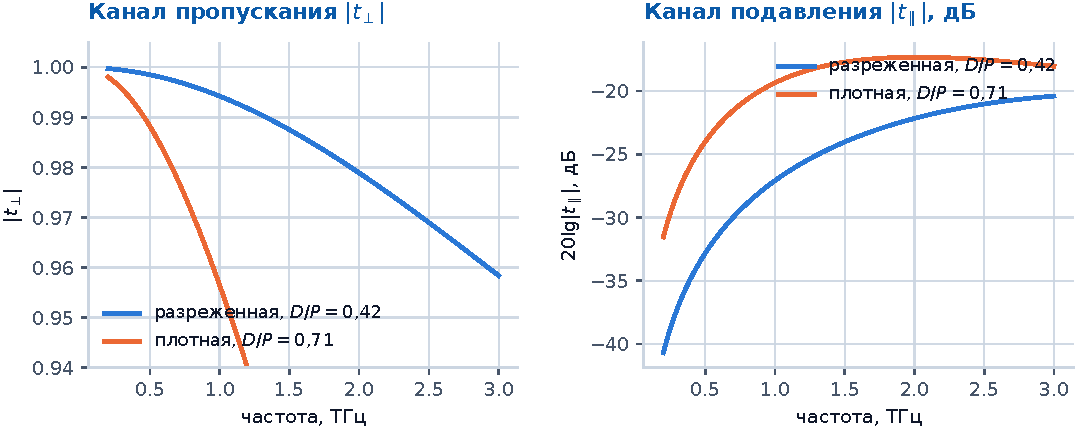
\includegraphics[width=\linewidth]{figures/fig02_transmission.pdf}
  \caption{Модельный расчёт $\tperp(\nu)$ и $\tpar(\nu)$ по формулам
  §§\ref{subsec:A1A2}--\ref{subsec:transmission} (без учёта конечной проводимости провода~---
  этот эффект вносится отдельным следующим слоем модели) для двух плотностей решётки на рабочей
  полосе частот.
  Канал пропускания уверенно держится у единицы независимо от плотности; канал подавления
  на порядки меньше и заметно чувствительнее к $D/P$.}
  \label{fig:blanco-spectrum}
\end{figure}

\begin{figure}[t]
  \centering
  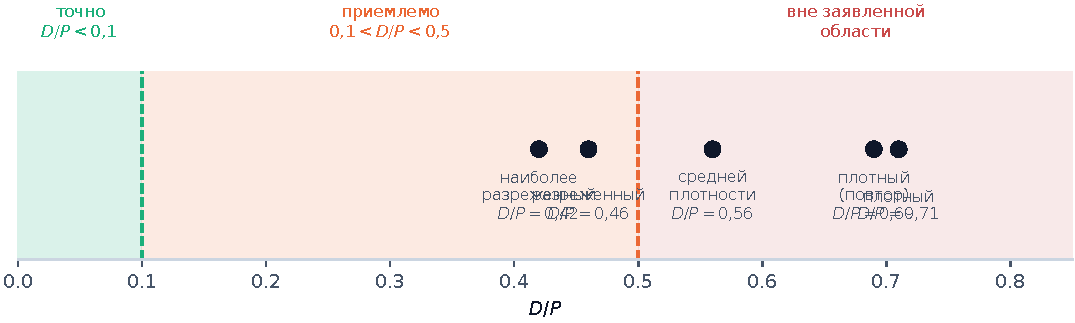
\includegraphics[width=\linewidth]{figures/fig02_validity_map.pdf}
  \caption{Карта применимости по параметру плотности $D/P$: узкая заявленная область точности,
  смягчённая граница приемлемости, область за пределами обеих и положение измеренных образцов
  (ключ~2.2). Условие $D/\lambda<0{,}2$ на этой оси не показано~--- оно выполнено для всех
  образцов с большим запасом на всей рабочей полосе частот (см. текст).}
  \label{fig:validity-map}
\end{figure}

% ---------------------------------------------------------------------
\subsection{Типичные ошибки этого параграфа}

\begin{enumerate}[leftmargin=1.6em,itemsep=0.25em]
  \item Спутать амплитудные коэффициенты $\tperp,\tpar$ с публикуемыми в первоисточнике
        мощностными $K_1,K_2$~--- та же ошибка на множитель два в децибелах, что и в
        §\ref{subsec:leakage}, только на входе модели.
  \item Проверять только $D/P<0{,}5$ и забыть про независимое условие $D/\lambda<0{,}2$~---
        оба должны выполняться одновременно.
  \item Считать резкой границей то, что на самом деле~--- постепенная потеря точности разложения
        по малому параметру; за формальной границей модель не обязана быть <<неверной>>, но
        доверие к ней требует отдельной проверки.
  \item Приписывать вещественную часть импеданса омическим потерям в проводе. В этой модели
        провод идеально проводящий; вещественная часть (недостижимая в нашей полосе частот)
        означает перекачку энергии в эванесцентные дифракционные порядки, а не нагрев.
  \item Забыть, что оба канала строятся из \emph{одних и тех же} чисел $A_1,A_2$~--- это не два
        независимых расчёта, а два разных сочетания одного и того же геометрического
        содержания.
\end{enumerate}

\clearpage
               % §2  Модель Бланко: откуда берутся t_perp и t_par    [ГОТОВ]
% % =====================================================================
%  §3. Материальные поправки: Друде и рассеяние ν^γ
%
%  ЖАНР (STYLE.md): учебная литература. Ни путей, ни имён программ, ни
%  номеров гипотез. Прослеживаемость — ключи \srckey{3.x} и приложение.
%
%  Содержательная основа: BRIEF_FOR_D_teaching_ladder.md §4; SYNTHESIS.md
%  §4-5 (реестр гипотез HN5/HN11 с ΔAIC).
% =====================================================================
\section{Материальные поправки: Друде и рассеяние \texorpdfstring{$\nu^\gamma$}{nu\^{}gamma}}
\label{sec:drude}
\markboth{§\thesection. Друде и рассеяние}{}

Модель §\ref{sec:blanco} считала провод \textbf{идеально проводящим}: вся его роль сводилась к
геометрии, а вещественная часть импеданса появлялась только за счёт эванесцентных дифракционных
порядков (и в нашей полосе частот она равна нулю). Настоящий провод сделан из настоящего металла
с конечной проводимостью, и это добавляет два независимых физических эффекта, которые нужно
внести в модель \emph{поверх} геометрии Бланко. Этот параграф вводит оба и заканчивается уроком,
который пригодится для всей оставшейся части курса: улучшение согласия с данными и измеримость
параметра, отвечающего за это улучшение,~--- разные вещи.

\begin{tcolorbox}[enhanced,colback=cPanel,colframe=cGrid,boxrule=0.8pt,arc=2pt,
                  title={\bfseries\color{cAccent} Пререквизиты},coltitle=cAccent,
                  attach boxed title to top left={xshift=6pt,yshift=-2pt},
                  boxed title style={colback=cPanel,boxrule=0pt,arc=0pt},top=10pt]
\textbf{Нужно знать:} §\ref{sec:blanco} (эквивалентная схема, реактивные импедансы, откуда
берутся $\tperp,\tpar$); комплексный импеданс; понятие проводимости металла.\\[0.3em]
\textbf{Знать НЕ нужно:} микроскопическую теорию электронного транспорта. Модель Друде вводится
здесь на уровне одной формулы для поверхностного импеданса, без вывода из кинетического
уравнения.
\end{tcolorbox}

% ---------------------------------------------------------------------
\subsection{Конечная проводимость: поверхностный импеданс металла}
\label{subsec:drude-impedance}

\begin{intuition}
Идеальный проводник экранирует поле мгновенно и без потерь: поверхностный ток течёт строго по
поверхности, вглубь ничего не проникает. Настоящий металл~--- не идеальный проводник: поле
проникает на конечную глубину (скин-слой), там совершает работу над электронами, и часть энергии
уходит в тепло. С точки зрения внешней волны это выглядит как \emph{малый} дополнительный
импеданс на поверхности провода~--- не ноль, но и не большая величина, потому что металл всё же
хороший проводник на терагерцовых частотах.
\end{intuition}

\noindent
\term{Модель Друде} описывает проводимость металла как отклик свободных электронов с временем
релаксации $\tau_e$ (среднее время между столкновениями электрона с решёткой):
\begin{equation}
  \sigma(\omega)=\frac{\sigma_0}{1-\jj\omega\tau_e},
  \qquad
  Z_s(\omega)=\sqrt{\frac{\jj\omega\mu_0}{\sigma(\omega)}},
  \label{eq:drude}
\end{equation}
где $\sigma_0$~--- проводимость на постоянном токе, $\mu_0$~--- магнитная проницаемость вакуума,
$Z_s$~--- \term{поверхностный импеданс}, нормируемый на импеданс вакуума $Z_0$. Эта величина
входит в эквивалентную схему §\ref{sec:blanco} как малая добавка к реактивным импедансам
$Z_a,\ldots,Z_d$~--- на тех же местах, где раньше стоял чистый ноль.

\begin{strict}[: почему добавка малая и почему она комплексная]
На терагерцовых частотах $\omega\tau_e\ll1$ для типичных металлов ($\tau_e$~--- порядка
$10^{-14}$~с), поэтому $\sigma(\omega)\approx\sigma_0$ почти вещественна, а
$Z_s\propto\sqrt{\omega/\sigma_0}$~--- мала и растёт с частотой. Комплексность $Z_s$ означает, что
добавка вносит не только затухание (вещественная часть~--- омические потери, то, чего не было в
идеальном проводнике §2), но и малый дополнительный фазовый сдвиг (мнимая часть). Оба эффекта
одного порядка малости и одного физического происхождения~--- конечная проводимость,~--- поэтому
вводятся одной формулой, а не двумя независимыми поправками.
\end{strict}

\begin{warning}[: это не то же самое, что просачивание из §1]
Поправка Друде действует \textbf{одинаково на оба канала}~--- она модифицирует геометрическую
схему §2 целиком, а не создаёт новый путь для поля. Просачивание $\tpar$ (§\ref{subsec:leakage})
существовало бы даже для идеально проводящего провода~--- оно геометрическое, от неполноты
экранирования узкой решёткой. Друде добавляет к обоим каналам небольшую частотно-зависимую
поправку сверху, не создавая канал заново.
\end{warning}

% ---------------------------------------------------------------------
\subsection{Степенное рассеяние: феноменологический член потерь}
\label{subsec:power-law}

Поправка Друде объясняет часть отклонений от идеального проводника, но не все: после её включения
в модели остаётся систематический, гладкий по частоте остаток~--- амплитуда прошедшего поля падает
с частотой чуть быстрее или медленнее, чем предсказывает \eqref{eq:drude}. Стандартный приём~---
добавить \term{феноменологический} множитель потерь, не привязанный к конкретному микроскопическому
механизму:
\begin{equation}
  a_{\text{потери}}(\nu)=\exp\!\Big[-\tfrac12\,\tfrac{L}{4{,}343}\,\nu^{\gamma}\Big],
  \label{eq:power-law-loss}
\end{equation}
где $L$~--- амплитудный коэффициент потерь (во сколько децибел на единицу частотной шкалы), а
$\gamma$~--- показатель степени. Множитель $1/4{,}343=\ln10/10$ переводит децибелы в натуральный
показатель экспоненты.

\begin{intuition}
Классическое рэлеевское рассеяние на неоднородностях масштаба меньше длины волны даёт $\gamma=2$
(квадратичный рост потерь с частотой)~--- это своего рода <<умолчание>>, если механизм потерь не
уточняется. Но реальные механизмы (рассеяние на границах зёрен металла, эффект Фукса--Зондхаймера
в тонких проводящих слоях и другие) дают показатели, отличные от двух, причём часто дробные. Вместо
того чтобы выбирать один механизм заранее, формула~\eqref{eq:power-law-loss} оставляет $\gamma$
свободным параметром и позволяет данным сказать, какой показатель им нужен.
\end{intuition}

% ---------------------------------------------------------------------
\begin{figure}[t]
  \centering
  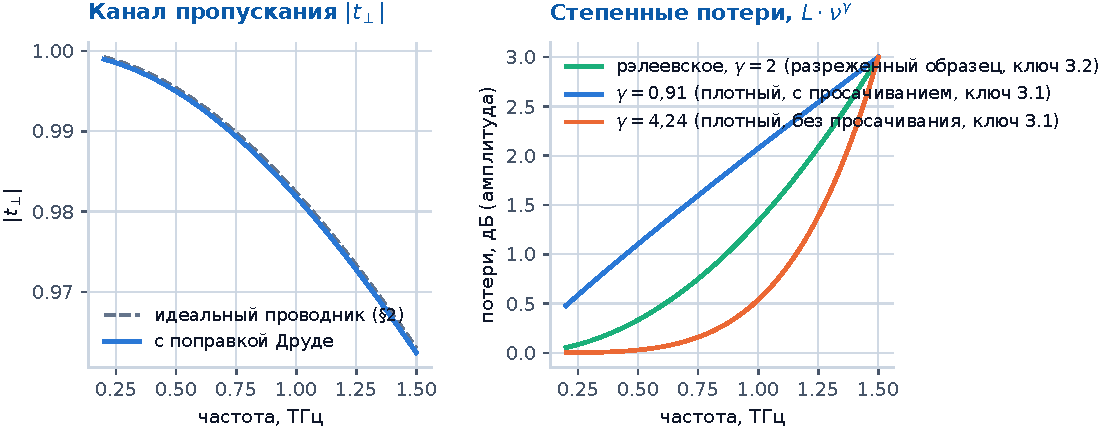
\includegraphics[width=\linewidth]{figures/fig03_drude.pdf}
  \caption{Модельный расчёт. Слева: канал пропускания с поправкой Друде и без неё (формула
  §\ref{subsec:drude-impedance} поверх геометрии §2, $D/P=0{,}56$)~--- отличие на рабочей полосе
  составляет тысячные доли и на глаз не заметно. Справа: множитель степенных потерь
  \eqref{eq:power-law-loss} для трёх показателей~$\gamma$, включая два значения из
  примера~\ref{subsec:no-measurement} (одна и та же величина потерь на верхней границе полосы,
  разный ход по частоте).}
  \label{fig:drude}
\end{figure}

% ---------------------------------------------------------------------
\subsection{«Эффект есть — параметр не измерен»}
\label{subsec:no-measurement}

Добавление члена~\eqref{eq:power-law-loss} к модели §2$+$Друде реально и заметно улучшает
согласие с данными. Возникает естественный вопрос: раз модель стала лучше, значит ли это, что мы
\emph{измерили} показатель рассеяния~$\gamma$? Ответ~--- поучительное <<нет>>, и разбор того, почему
именно нет, стоит того, чтобы задержаться.

\begin{example}[: улучшение согласия реально]\srckey{3.1}
На плотной решётке ($D/P=0{,}71$) добавление степенного члена потерь улучшает информационный
критерий на $\dAIC\approx-733$ относительно модели без него (шкала $\dAIC$ разбирается в §8;
здесь достаточно знать, что такая величина~--- уверенное, не случайное улучшение). Эффект
проверен и признан реальным.
\end{example}

\begin{warning}[: но сам показатель $\gamma$ плывёт]
На тех же данных значение $\gamma$ существенно зависит от того, включена ли в модель одновременно
явная поправка на просачивание (§\ref{subsec:leakage}, будет формально введена в модель в §6):
с учётом просачивания $\gamma\approx0{,}91$, без него~--- $\gamma\approx4{,}24$. Это не опечатка и
не ошибка подгонки~--- это \emph{один и тот же} набор данных, дающий вчетверо-впятеро разные оценки
одного и того же параметра в зависимости от соседнего слагаемого модели.
\end{warning}

\begin{intuition}[: почему так происходит]
Оба члена~--- степенные потери и просачивание~--- на верхних частотах рабочей полосы производят
похожий на вид эффект: плавный дополнительный спад амплитуды с частотой в канале подавления. Когда
в модели нет явного просачивания, показателю~$\gamma$ приходится \emph{за двоих} воспроизводить
форму спада, которая на самом деле частично принадлежит другому физическому механизму. Показатель
степени становится <<мусорной корзиной>>: он подстраивается под любую гладкую форму спада, доступную
модели, независимо от того, какой физический процесс её на самом деле создал.
\end{intuition}

\begin{example}[: на разреженном образце показатель ведёт себя иначе]\srckey{3.2}
На самом разреженном из образцов, где просачивание слабее выражено (§\ref{sec:electrodynamics}),
показатель определяется гораздо увереннее~--- $\gamma\approx2{,}04$ с узким интервалом
$[1{,}96;\,2{,}15]$~--- и близок к классическому рэлеевскому значению~$2$. Проверка того, общий ли
это показатель для всех образцов (единая материальная константа, не зависящая от конкретной
решётки), пока не подтверждена: слишком мало образцов дают устойчивую оценку, чтобы делать вывод
об универсальности.
\end{example}

\begin{tcolorbox}[enhanced,colback=cS1!7,colframe=cS1,boxrule=0pt,leftrule=3pt,arc=1pt]
\textbf{Различение, которое стоит запомнить на весь курс.} \emph{«Модель с этим членом лучше
описывает данные»} и \emph{«численное значение этого параметра надёжно»} — два разных
утверждения, и первое не влечёт второго. Эффект существует и достоверен ($\dAIC=-733$); конкретное
число, которым модель его описывает, зависит от того, что ещё присутствует в модели рядом, и может
меняться в разы. Курс вернётся к этому различению как к общему методическому правилу в §8--§9 и как
к готовому рабочему принципу в §10.
\end{tcolorbox}

% ---------------------------------------------------------------------
\subsection{Типичные ошибки этого параграфа}

\begin{enumerate}[leftmargin=1.6em,itemsep=0.25em]
  \item Считать поправку Друде источником просачивания. Это независимые эффекты: Друде~---
        конечная проводимость, действует на оба канала одинаково; просачивание~--- геометрическая
        неполнота экранирования, создаёт новый путь для поля (§\ref{subsec:drude-impedance}).
  \item Принять улучшение $\dAIC$ от степенного члена потерь за измерение показателя~$\gamma$.
        Улучшение согласия и определённость параметра, отвечающего за него,~--- разные вопросы
        (§\ref{subsec:no-measurement}).
  \item Забыть проверить, с чем ещё в модели конкурирует новый параметр, прежде чем доверять его
        числовому значению. Оценка $\gamma$ вчетверо меняется от присутствия соседнего члена
        модели.
  \item Обобщать оценку показателя рассеяния с одного образца на все остальные без проверки: пока
        это не подтверждено.
\end{enumerate}

\clearpage
              % §3  Друде и рассеяние nu^gamma: частотная зависимость

% =====================================================================
%  ЧАСТЬ II. ОЦЕНИВАНИЕ: от линейного фита к нелинейному
%  ВНИМАНИЕ: порядок 04 -> 05 -> 06 -> 07 менять нельзя. Корреляция
%  вводится на линейном примере, где она в замкнутой форме, и лишь
%  затем переносится на нелинейное вырождение D_eff <-> eta_0.
% =====================================================================
% \part*{Часть II. Оценивание параметров}
% \addcontentsline{toc}{section}{\textbf{Часть II. Оценивание параметров}}

% % =====================================================================
%  §4. Линейная аппроксимация: гармоники закона Малюса
%
%  ЖАНР (STYLE.md): учебная литература. Ни путей, ни имён программ, ни
%  номеров гипотез. Прослеживаемость — ключи \srckey{4.x} и приложение.
%
%  Содержательная основа: research/two_wgp/NOTE_malus_linearization.md
%  (обучающий разбор с выводом; markdown первичен по фактуре).
% =====================================================================
\section{Линейная аппроксимация: гармоники закона Малюса}
\label{sec:linear-fit}
\markboth{§\thesection. Линейная аппроксимация}{}

Части~II этого курса предстоит подгонять модель к измеренной угловой развёртке~--- в общем случае
нелинейную задачу с итерациями, стартовыми точками и риском застрять не в том решении
(аппарат для этого появится в §7). Но прежде чем разбираться с этими трудностями, стоит заметить:
часть той же самой информации~--- офсет угла, амплитуды каналов, их относительная
фаза~--- извлекается \emph{без единой итерации}, обычным линейным методом наименьших квадратов, с
единственным глобальным минимумом и точной, а не приближённой, оценкой ошибки. Это не хитрость и
не частный случай~--- это следствие одного тригонометрического тождества, применённого к
выражению~\eqref{eq:two-channels}, которое курс вывел ещё в §0.

\begin{tcolorbox}[enhanced,colback=cPanel,colframe=cGrid,boxrule=0.8pt,arc=2pt,
                  title={\bfseries\color{cAccent} Пререквизиты},coltitle=cAccent,
                  attach boxed title to top left={xshift=6pt,yshift=-2pt},
                  boxed title style={colback=cPanel,boxrule=0pt,arc=0pt},top=10pt]
\textbf{Нужно знать:} формулы~\eqref{eq:two-channels}--\eqref{eq:U-cross} из §0 (поле~$\Efield(\theta)$
и энергия~$U(\theta)$ с перекрёстным членом); тригонометрическая формула понижения степени
$\cos^2\alpha=\tfrac12(1+\cos2\alpha)$; метод наименьших квадратов как решение нормального
уравнения линейной регрессии.\\[0.3em]
\textbf{Знать НЕ нужно:} нелинейную оптимизацию, алгоритм Левенберга--Марквардта~--- в этом
параграфе он не нужен вовсе, и это главная мысль параграфа.
\end{tcolorbox}

% ---------------------------------------------------------------------
\subsection{Идея: неудобная нелинейность на самом деле не нелинейность}
\label{subsec:idea}

\begin{intuition}
Классический закон Малюса записывают как «яркость~--- квадрат косинуса угла». Квадрат косинуса
выглядит неудобно: сам по себе он нелинеен по углу~$\theta$, а офсет~$\theta_0$~--- неизвестный
ноль шкалы прибора~--- сидит \emph{внутри} косинуса, что обычно требует итерационной подгонки.
Но школьное тождество $\cos^2\alpha=\tfrac12(1+\cos2\alpha)$ говорит: квадрат косинуса~--- это не
нелинейность, а косинус \emph{удвоенного} угла плюс константа. Модуляция происходит на удвоенной
частоте вращения~--- поворот на $180^\circ$ возвращает картину в исходное состояние, потому что
поляризатор не различает <<вперёд>> и <<назад>>.
\end{intuition}

Возьмём учебную (интенсивностную) форму закона Малюса, $U(\theta)=U_{\min}+(U_{\max}-U_{\min})
\cos^2(\theta-\theta_0)$, и применим тождество:
\begin{equation}
  U(\theta)=a_0+a_1\cos2\theta+b_1\sin2\theta,
  \label{eq:linear3}
\end{equation}
где $a_0=\tfrac12(U_{\max}+U_{\min})$, а $a_1,b_1$~--- некоторая пара чисел, зависящая от
$U_{\max}-U_{\min}$ и~$\theta_0$ (явные формулы~--- в §\ref{subsec:closed-form}).

\begin{strict}[: что произошло с офсетом]
Неизвестный угол~$\theta_0$ был аргументом косинуса~--- нелинейным параметром. После разложения он
«вышел наружу» и распределился между двумя \emph{линейными} коэффициентами $a_1,b_1$. Базисные
функции $1,\cos2\theta,\sin2\theta$ от неизвестных параметров не зависят~--- это фиксированный,
заранее известный набор функций угла. Значит, \eqref{eq:linear3}~--- обычная линейная регрессия, а
не итерационная задача.
\end{strict}

\begin{intuition}[: это стандартный приём метрологии]
Тот же самый ход~--- искать неизвестный офсет не подгонкой аргумента, а разложением по гармоникам
удвоенного угла~--- давно применяется в оптической метрологии вращающегося элемента (эллипсометрия
с вращающимся анализатором, синхронное детектирование на второй гармонике). Курс применяет его не
ко времени, а к угловой развёртке~--- идея та же.
\end{intuition}

% ---------------------------------------------------------------------
\subsection{Почему нужна четвёртая гармоника}
\label{subsec:fourth-harmonic}

Форма~\eqref{eq:linear3}~--- учебная: она верна для \emph{некогерентной} (интенсивностной)
композиции каналов. Но §0 установил (формула~\eqref{eq:two-channels}), что наша установка
складывает \emph{поля}, а не мощности, и лишь потом берёт квадрат модуля. Применим то же
тождество понижения степени прямо к полю:
\begin{equation}
  \Efield(\theta)=\tperp\cos^2\theta+\tpar\sin^2\theta
  = A+B\cos2\theta,
  \qquad
  A=\tfrac12(\tperp+\tpar),\quad B=\tfrac12(\tperp-\tpar).
  \label{eq:field-linear}
\end{equation}
Поле линейно по $\cos2\theta$~--- многочлен первой степени. Но наблюдаемая~--- это
$U=|\Efield|^2$, а квадрат многочлена первой степени по $\cos2\theta$ содержит $\cos^22\theta$,
которое тем же тождеством понижения степени даёт $\cos4\theta$. Итого \textbf{точно}, без всякого
приближения:
\begin{equation}
  U(\theta)=c_0+a_2\cos2\theta+b_2\sin2\theta+a_4\cos4\theta+b_4\sin4\theta .
  \label{eq:linear5}
\end{equation}

\begin{warning}[: это тождество, а не аппроксимация]
Разложение~\eqref{eq:linear5} не отбрасывает никаких членов и не является рядом, обрезанным на
каком-то порядке. Квадрат модуля линейной по $\cos2\theta$ величины~--- \emph{ровно}
тригонометрический многочлен 4-й степени, и точнее пяти коэффициентов~\eqref{eq:linear5} для его
описания не требуется. Это ровно то же тождество, что дало формулу~\eqref{eq:U-cross} в §0, только
здесь оно доведено до готового линейного базиса.
\end{warning}

\begin{example}[: точность тождества на практике]\srckey{4.1}
Прямая численная проверка формы~\eqref{eq:linear5} против полного выражения~\eqref{eq:U-cross} на
измеренных частотных сетках даёт относительное среднеквадратичное расхождение порядка
$10^{-16}$~--- машинный ноль (тот же результат, что уже приводился в §0 как ключ~0.2, здесь~---
подтверждение того, что он справедлив построчно, на уровне отдельной частоты, а не только в
среднем).
\end{example}

\begin{tcolorbox}[enhanced,colback=cS1!7,colframe=cS1,boxrule=0pt,leftrule=3pt,arc=1pt]
\textbf{Учебная 3-параметрическая форма~\eqref{eq:linear3} для нашей установки систематически
неполна}: она отбрасывает четвёртую гармонику, которая, как было установлено в §0, несёт около
четверти всего сигнала~--- и, что важнее, несёт единственную информацию об относительной фазе
каналов (следующий пункт).
\end{tcolorbox}

% ---------------------------------------------------------------------
\subsection{Замкнутые формулы: от коэффициентов обратно к физике}
\label{subsec:closed-form}

Три коэффициента $c_0,c_2,c_4$ (где $c_2=\sqrt{a_2^2+b_2^2}$, $c_4$~--- аналогично для четвёртой
гармоники, с точностью до знака, обсуждаемой ниже) связаны с тремя физическими величинами
взаимно однозначно:
\begin{equation}
  |\tperp|^2=c_0+c_2+c_4,
  \qquad
  |\tpar|^2=c_0-c_2+c_4,
  \qquad
  \Real(\tperp\overline{\tpar})=c_0-3c_4 .
  \label{eq:closed-form}
\end{equation}
Отсюда~--- \term{модельно-независимо}, одним решением линейной системы, без какого-либо
предположения о механизме, породившем $\tperp,\tpar$:
\[
  \eta=\left|\frac{\tpar}{\tperp}\right|
  =\sqrt{\frac{c_0-c_2+c_4}{c_0+c_2+c_4}},
  \qquad
  \cos\Delta\varphi=\frac{c_0-3c_4}{\sqrt{(c_0+c_2+c_4)(c_0-c_2+c_4)}} .
\]

\begin{intuition}[: самый красивый момент этого параграфа]
Относительная фаза каналов $\Delta\varphi$~--- физическая величина, за которой мы гонялись ещё с
§0 ($\tleak$~--- это её наклон по частоте,~--- и с §1, где просачивание получило и амплитуду,
и фазу,~--- входит в формулы \eqref{eq:closed-form} \textbf{только через}~$c_4$. В интенсивностной
трёхпараметрической картине фазы нет вообще~--- она там принципиально ненаблюдаема. Учебная
линеаризация~\eqref{eq:linear3} слепа к $\Delta\varphi$ не приблизительно, а точно: она
выбрасывает ровно ту гармонику, которая единственная её несёт.
\end{intuition}

\begin{strict}[: два бесплатных теста корректности]
Формулы~\eqref{eq:closed-form} дают два внутренних теста, которых нет в нелинейной подгонке:
\begin{enumerate}[leftmargin=1.6em,itemsep=0.2em]
  \item \term{Неравенство Коши--Буняковского} $|\Real(\tperp\overline{\tpar})|\le|\tperp||\tpar|$,
        то есть $|\cos\Delta\varphi|\le1$. Нарушение означает, что данные не описываются схемой
        «один вращающийся элемент, дающий поле по формуле~\eqref{eq:field-linear}»~--- сигнал
        каких-либо помех к сигналу.
  \item \term{Согласие двух независимых оценок офсета}: $\theta_0=\tfrac12\operatorname{atan2}(b_2,a_2)$
        из второй гармоники и $\theta_0=\tfrac14\operatorname{atan2}(b_4,a_4)\pmod{45^\circ}$ из
        четвёртой обязаны совпасть, если данные действительно порождены одним и тем же
        вращающимся элементом.
\end{enumerate}
\end{strict}

% ---------------------------------------------------------------------
\begin{figure}[t]
  \centering
  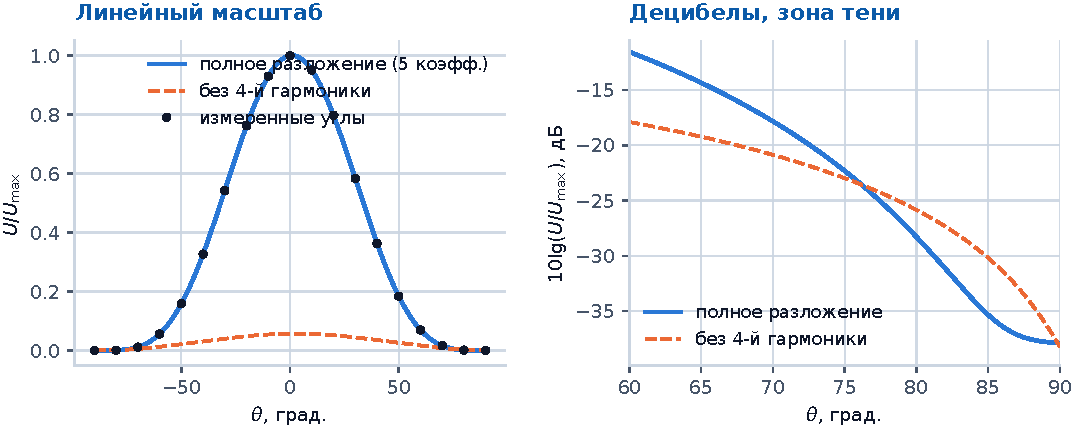
\includegraphics[width=\linewidth]{figures/fig04_harmonics_decomp.pdf}
  \caption{Плотная решётка ($D/P=0{,}71$, ключ~4.2): измеренная угловая развёртка (энергия,
  просуммированная по рабочей полосе частот) и её восстановление по формуле~\eqref{eq:linear5} со
  всеми пятью коэффициентами против восстановления без четвёртой гармоники. В районе максимумов
  разница не видна; вблизи $90^\circ$, где сосредоточено просачивание, отбрасывание четвёртой
  гармоники даёт заметный систематический сдвиг~--- та же четверть сигнала, о которой шла речь
  выше, теряется именно там, где она важнее всего.}
  \label{fig:harmonics-decomp}
\end{figure}

% ---------------------------------------------------------------------
\subsection{Аппарат линейного МНК}
\label{subsec:lsq}

Запишем~\eqref{eq:linear5} как задачу линейной регрессии. Пусть измерено $N$ значений $U_i$ на
углах~$\theta_i$. \term{Матрица плана}~$X$ имеет $N$ строк и пять столбцов:
\[
  X=\big[\,1,\ \cos2\theta_i,\ \sin2\theta_i,\ \cos4\theta_i,\ \sin4\theta_i\,\big]_{i=1\ldots N},
\]
и решение~--- обычные нормальные уравнения взвешенного МНК:
\begin{equation}
  \mathbf{p}=(X^{\mathsf T}WX)^{-1}X^{\mathsf T}W\mathbf{y},
  \qquad
  \operatorname{Cov}(\mathbf{p})=(X^{\mathsf T}WX)^{-1},
  \qquad
  W=\operatorname{diag}(1/\sigma_i^2) .
  \label{eq:normal-eq}
\end{equation}
Ни итераций, ни стартовой точки, ни риска сойтись не туда: система линейна, решение~--- одно
решение линейной алгебры, ковариация~--- точная (не приближение вблизи минимума, как это будет
в §7--§9 для нелинейной задачи).

\begin{intuition}[: откуда берётся ковариация без всякой статистики Монте-Карло]
Для линейной регрессии с гауссовым шумом оценка коэффициентов~$\mathbf{p}$~--- сама линейная
комбинация данных, и её ковариация выражается через ковариацию данных \emph{в замкнутом виде}
матричной формулой $(X^{\mathsf T}WX)^{-1}$. Бутстрап или другие ресемплинговые методы (§7) здесь
попросту не нужны~--- они нужны там, где такой формулы нет.
\end{intuition}

\paragraph{Дельта-метод.} Величины вроде $\theta_0$~--- нелинейные функции коэффициентов
$a_2,b_2$, и напрямую их ковариация из~\eqref{eq:normal-eq} не следует. Но раз ковариация
коэффициентов известна точно, ошибку любой гладкой функции от них~--- в частности,
$\theta_0=\tfrac12\operatorname{atan2}(b_2,a_2)$~--- даёт стандартный \term{дельта-метод}
(линеаризация функции первой производной):
\[
  \sigma^2(\theta_0)=\frac{b_2^2\operatorname{Var}(a_2)+a_2^2\operatorname{Var}(b_2)
  -2a_2b_2\operatorname{Cov}(a_2,b_2)}{4(a_2^2+b_2^2)^2} .
\]
В частном, но практически важном случае~--- углы равномерно покрывают полный период по
$2\theta$~--- матрица $X^{\mathsf T}X$ диагональна, и формула сворачивается до
$\sigma(\theta_0)=\sigma_U/(c_2\sqrt{2N})$: точность офсета определяется отношением шума к
амплитуде модуляции и числом точек~--- простая и полезная оценка при планировании измерения.

% ---------------------------------------------------------------------
\subsection{Урок про веса: шкала, в которой вы смотрите на данные, решает, что вы способны измерить}
\label{subsec:weights}

Матрица~$X$ не зависит от данных, но веса~$W$ выбираются, и выбор небезобиден.

\begin{warning}[: невзвешенный МНК заглушает тень]
Невзвешенный МНК по энергии эффективно взвешивает точку пропорционально~$U_i^2$ (обычная сумма
квадратов невязок весит большие значения тяжелее). Яркая зона (канал пропускания, малые углы)
на два--три порядка превосходит по величине тень (канал подавления, углы вблизи $90^\circ$)~---
и невзвешенный фит попросту не замечает тень, хотя именно там сосредоточена вся информация о
просачивании (§\ref{subsec:leakage}).
\end{warning}

\begin{example}[: до какой степени это ломает результат]\srckey{4.3}
На одном из образцов с относительно слабым просачиванием невзвешенная подгонка дала
$|\tpar|^2<0$~--- физически невозможный результат: оценка энергии отрицательна. Это не сбой
арифметики, а прямое следствие того, что тень, где $|\tpar|^2$ реально определяется, была
статистически невидима для невзвешенного МНК.
\end{example}

\noindent
Решение~--- веса $\sigma_i\propto U_i$ (постоянная \emph{относительная} ошибка, а не абсолютная).
Задача остаётся линейной: веса не зависят от искомых параметров, только от самих измерений,
поэтому формула~\eqref{eq:normal-eq} применяется без изменений.

\begin{example}[: два независимых теста сходятся до сотых долей градуса]\srckey{4.4}
При относительном взвешивании два независимых способа оценить офсет~--- из второй гармоники и из
четвёртой (тест из §\ref{subsec:closed-form}) сходятся с точностью
$0{,}004^\circ$--$0{,}05^\circ$ на всех образцах, для которых есть измерения. Совпадение,
полученное \emph{без единого предположения о верности физической модели}~--- просто как следствие
внутренней непротиворечивости данных,~--- сильный аргумент за то, что развёртка действительно
описывается одним вращающимся элементом.
\end{example}

\begin{center}
\footnotesize
\setlength{\tabcolsep}{6pt}
\begin{tabular}{@{}lrrrr@{}}
\toprule
\textbf{Образец} & \textbf{$\theta_0$, равном.} & \textbf{$\theta_0$, относит.} & \textbf{$\eta$,
равном.} & \textbf{$\eta$, относит.}\\
\midrule
плотная решётка, $D/P=0{,}71$        & $-0{,}097^\circ$ & $+0{,}901^\circ\pm0{,}184$ & $0{,}0347$ & $0{,}0127$ \\
повторная установка, $D/P=0{,}69$ (а) & $-0{,}286^\circ$ & $-0{,}546^\circ\pm0{,}248$ & \emph{отриц.} & $0{,}0121$ \\
повторная установка, $D/P=0{,}69$ (б) & $-0{,}654^\circ$ & $-0{,}463^\circ\pm0{,}198$ & $0{,}0478$ & $0{,}0130$ \\
разреженный образец, $D/P=0{,}46$    & $+0{,}211^\circ$ & $+0{,}599^\circ\pm0{,}327$ & $0{,}0373$ & $0{,}0329$ \\
\bottomrule
\end{tabular}
\end{center}
\srckey{4.5}
\noindent\emph{«Равномерные» веса~--- $\sigma_i=\mathrm{const}$; «относительные»~---
$\sigma_i\propto U_i$. Ошибка $\theta_0$~--- дельта-метод, поправленный на неизвестный масштаб
шума данных (поправка Бирджа); бутстрап не требуется. У образца (а) равномерные веса дают
физически невозможную (отрицательную) оценку энергии тени, поэтому столбец $\eta$ для него пуст.}

% ---------------------------------------------------------------------
\begin{figure}[t]
  \centering
  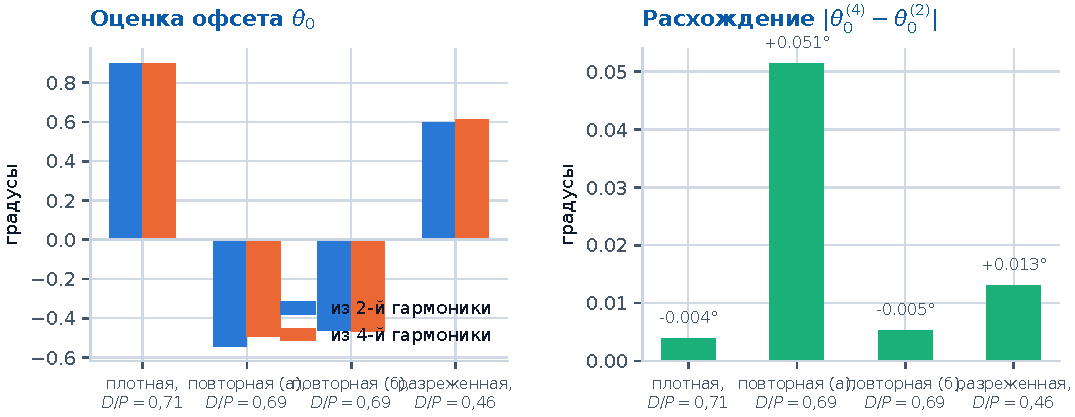
\includegraphics[width=\linewidth]{figures/fig04_weights.pdf}
  \caption{Согласие двух независимых оценок офсета~--- из второй и из четвёртой гармоники
  (§\ref{subsec:closed-form})~--- при относительном взвешивании $\sigma_i\propto U_i$: разница
  на всех образцах не превышает сотых долей градуса. Это внутренний тест непротиворечивости,
  а не сравнение с какой-либо независимо известной величиной.}
  \label{fig:weights}
\end{figure}

\begin{tcolorbox}[enhanced,colback=cS1!7,colframe=cS1,boxrule=0pt,leftrule=3pt,arc=1pt]
\textbf{Правило, впервые сформулированное в §1 (ключ~1.1) и подтверждённое здесь числом.} Шкала,
в которой вы взвешиваете данные, определяет, какие параметры вы способны измерить. Здесь это не
абстрактный тезис, а конкретная развилка: одни и те же измерения дают то отрицательную (невозможную)
оценку энергии тени, то физически осмысленный результат, совпадающий с независимой проверкой до
сотых долей градуса,~--- в зависимости только от выбора весов.
\end{tcolorbox}

% ---------------------------------------------------------------------
\subsection{Что ломает линейность, а что — нет}
\label{subsec:limits-linear}

Список того, что \emph{не} нарушает разложение~\eqref{eq:linear5} (доказано аналитически или
проверено численно), полезен не меньше списка ограничений: он избавляет от лишней осторожности
там, где она не нужна.

\begin{center}
\footnotesize
\setlength{\tabcolsep}{6pt}
\begin{tabular}{@{}p{0.34\linewidth}p{0.61\linewidth}@{}}
\toprule
\textbf{Не ломает} & \textbf{Почему} \\
\midrule
Частотная зависимость каналов & На каждой частоте своя пара $\tperp(\nu),\tpar(\nu)$~--- свои
$c_0,c_2,c_4$; структура~\eqref{eq:linear5} сохраняется частотно-поточечно \\
Фазовый член просачивания & Входит только в $\Real(\tperp\overline{\tpar})$, то есть только в
$c_4$; порядок многочлена не меняется \\
Суммирование по частотам & Сумма многочленов 4-й степени~--- снова многочлен 4-й степени \\
Второй (реальный) элемент тракта при выровненной оси & Теорема §\ref{subsec:alignment} даёт
общий скалярный множитель, не зависящий от $\theta$; отношения $\eta,\cos\Delta\varphi$ к нему
нечувствительны \\
\bottomrule
\end{tabular}
\end{center}

\begin{warning}[: а вот это ломает]
\textbf{Работа в децибелах.} Логарифм от тригонометрического многочлена~--- не многочлен: прямая
проверка даёт относительное расхождение порядка процента, когда та же процедура применяется к
$\lg U$ вместо~$U$. Разложение~\eqref{eq:linear5} нужно применять к самой энергии, а в
логарифмический масштаб переходить только для показа результата, не для его получения.
\textbf{Многолучевая интерференция} между элементами тракта тоже ломает структуру~--- она вносит
рациональную (а не полиномиальную) зависимость от $\cos2\theta$, то есть бесконечный ряд
гармоник; проверяется контролем гармоник шестого порядка и выше, которых в идентичности не
предусмотрено.
\end{warning}

% ---------------------------------------------------------------------
\subsection{Типичные ошибки этого параграфа}

\begin{enumerate}[leftmargin=1.6em,itemsep=0.25em]
  \item Использовать трёхпараметрическую (учебную) форму~\eqref{eq:linear3} для когерентной
        установки. Она отбрасывает четвёртую гармонику~--- четверть сигнала и всю фазу
        просачивания.
  \item Подгонять $\lg U$ или дБ вместо самой энергии~$U$. Логарифм многочлена~--- не многочлен;
        разложение перестаёт быть точным (§\ref{subsec:limits-linear}).
  \item Использовать одинаковые (не относительные) веса при большом динамическом диапазоне
        данных: яркая зона статистически заглушает тень, где сосредоточена вся интересующая
        физика (§\ref{subsec:weights}).
  \item Забыть проверить неравенство Коши--Буняковского для полученных $\tperp,\tpar$~--- это
        бесплатный тест, который нелинейная подгонка (§7) не предоставляет автоматически.
  \item Спутать согласие двух оценок офсета (внутренний тест непротиворечивости данных) с
        подтверждением физической модели: оно проверяет только то, что развёртку действительно
        произвёл один вращающийся элемент, а не то, какая модель верно описывает~$\tperp,\tpar$.
\end{enumerate}

\clearpage
         % §4  Линейная аппроксимация: гармоники закона Малюса
% % =====================================================================
%  §5. Корреляция как свойство плана эксперимента
%
%  ЖАНР (STYLE.md): учебная литература. Ни путей, ни имён программ, ни
%  номеров гипотез. Прослеживаемость — ключи \srckey{5.x} и приложение.
%
%  Содержательная основа: research/two_wgp/NOTE_malus_linearization.md §6;
%  BRIEF_FOR_D_teaching_ladder.md §6.
% =====================================================================
\section{Корреляция как свойство плана эксперимента}
\label{sec:correlation}
\markboth{§\thesection. Корреляция}{}

Формула ковариации~\eqref{eq:normal-eq} из §4 содержит $(X^{\mathsf T}WX)^{-1}$~--- матрицу,
целиком построенную из \emph{углов измерения} и весов, но не из самих измеренных значений. Это
не техническая деталь, а содержательный факт, который стоит вынести в отдельный параграф:
\textbf{насколько хорошо будут разделены параметры подгонки, известно ДО того, как получена хотя
бы одна точка данных}~--- достаточно знать, на каких углах прибор будет измерять. Здесь этот факт
проверяется на числах, вычислимых в закрытой форме, а в §9 тот же самый механизм вернётся в
гораздо менее наглядном виде~--- как вырождение параметров нелинейной модели.

\begin{tcolorbox}[enhanced,colback=cPanel,colframe=cGrid,boxrule=0.8pt,arc=2pt,
                  title={\bfseries\color{cAccent} Пререквизиты},coltitle=cAccent,
                  attach boxed title to top left={xshift=6pt,yshift=-2pt},
                  boxed title style={colback=cPanel,boxrule=0pt,arc=0pt},top=10pt]
\textbf{Нужно знать:} §4 целиком (матрица плана, нормальные уравнения, ковариация); что такое
собственные числа симметричной матрицы (на уровне интуиции: направления, в которых квадратичная
форма растёт быстрее или медленнее всего).\\[0.3em]
\textbf{Знать НЕ нужно:} численные методы решения плохо обусловленных систем~--- этот параграф про
то, как \emph{обнаружить} плохую обусловленность и что она означает, а не про то, как с ней
бороться вычислительно.
\end{tcolorbox}

% ---------------------------------------------------------------------
\subsection{Число обусловленности: одна цифра про качество плана}
\label{subsec:condition-number}

\begin{intuition}
Представьте матрицу $X^{\mathsf T}X$ как эллипсоид: чем он более вытянут, тем труднее по данным
различить движение вдоль его длинной оси от движения вдоль короткой~--- шум в любом направлении
неотличим от смеси обоих. \term{Число обусловленности} $\cond(X^{\mathsf T}X)$~--- отношение
наибольшего собственного числа к наименьшему~--- одним числом измеряет, насколько вытянут этот
эллипсоид. Число, близкое к единице,~--- эллипсоид почти круглый, направления равноправны; число,
на порядки больше единицы,~--- эллипсоид сильно вытянут, и в его <<узком>> направлении оценка
параметра ненадёжна, сколько бы ни было данных.
\end{intuition}

\begin{strict}
Для матрицы плана со столбцами $\{1,\cos2\theta,\sin2\theta,\cos4\theta,\sin4\theta\}$
обусловленность $X^{\mathsf T}X$ зависит только от того, \emph{на каких углах} стоят строки~---
то есть исключительно от плана измерения. Если столбцы (как функции на множестве измеренных
углов) взаимно ортогональны, $X^{\mathsf T}X$ диагональна и $\cond=1$; чем ближе какая-либо пара
столбцов к линейной зависимости (коллинеарности) на данном наборе углов, тем больше
$\cond(X^{\mathsf T}X)$, и тем хуже определены соответствующие коэффициенты.
\end{strict}

% ---------------------------------------------------------------------
\subsection{Две конфигурации одного и того же прибора}
\label{subsec:two-configs}

В проекте, на данных которого строится курс, угловая развёртка снималась либо на полном
симметричном диапазоне (примерно от $-90^\circ$ до $+90^\circ$), либо, в одном из режимов работы
установки, только на половине~--- от $0^\circ$ до $90^\circ$. Разница выглядит невинно: тот же шаг
по углу, просто вдвое меньше точек. Чистая геометрия матрицы плана говорит другое.

\begin{example}[: цена усечения диапазона, посчитанная без единого измерения]\srckey{5.1}
\begin{center}
\footnotesize
\setlength{\tabcolsep}{7pt}
\begin{tabular}{@{}lrrr@{}}
\toprule
\textbf{План} & \textbf{Углов} & $\cond(X^{\mathsf T}X)$ & $\sigma(\theta_0)$ при шуме $1\,\%$\\
\midrule
$-90^\circ\ldots+90^\circ$        & 19 & $\mathbf{2{,}14}$   & $\mathbf{0{,}096^\circ}$ \\
$0^\circ\ldots90^\circ$ & 10 & $\mathbf{236{,}3}$  & $\mathbf{0{,}944^\circ}$ \\
\bottomrule
\end{tabular}
\end{center}
Обусловленность хуже в сто с лишним раз, а точность офсета~--- почти в десять. Оба числа получены
из одной лишь геометрии множества углов~--- \emph{до} какого-либо измерения.
\end{example}

\begin{intuition}[: откуда берётся разница]
На полном симметричном диапазоне вторая и четвёртая гармоники угла почти ортогональны как функции
на множестве измеренных точек~--- максимальное перекрытие между ними всего около
$5\,\%$\srckey{5.1}. На диапазоне, обрезанном с одной стороны, симметрия множества углов
нарушена, и то же самое перекрытие вырастает до $37\,\%$\srckey{5.1}~--- гармоники перестают быть
почти независимыми измерениями, и матрица плана вытягивается в эллипсоид.
\end{intuition}

% ---------------------------------------------------------------------
\begin{figure}[t]
  \centering
  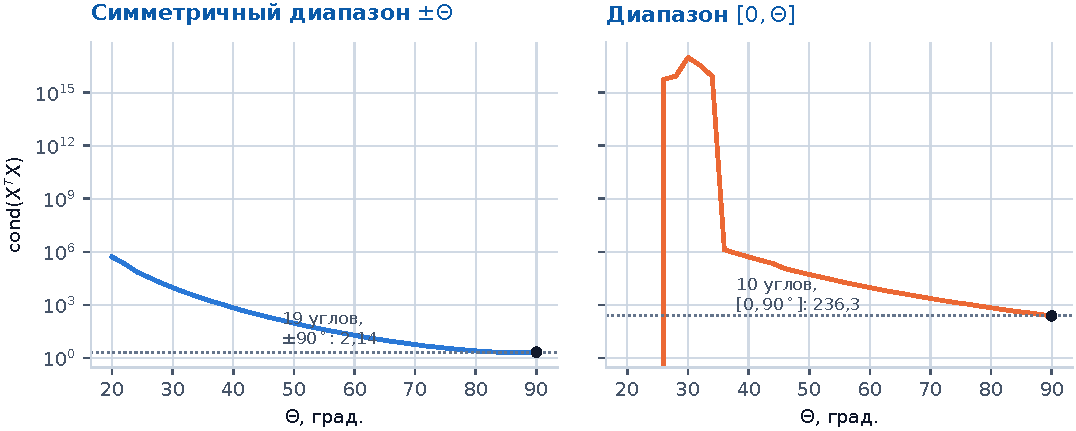
\includegraphics[width=\linewidth]{figures/fig05_cond_curve.pdf}
  \caption{Чистая геометрия матрицы плана (без каких-либо данных): $\cond(X^{\mathsf T}X)$ для
  пятигармонического базиса §4 как функция углового диапазона, при шаге между углами $10^\circ$.
  Слева: симметричный диапазон $\pm\Theta$. Справа: диапазон, зафиксированный с одной стороны в
  нуле, $[0,\Theta]$. Отмечены две конфигурации из таблицы примера~\ref{subsec:two-configs}.}
  \label{fig:cond-curve}
\end{figure}

% ---------------------------------------------------------------------
\subsection{Эллипс ковариации: та же геометрия, показанная напрямую}
\label{subsec:ellipse}

Число обусловленности~--- сводка одним числом; эллипс ковариации коэффициентов $(a_2,b_2)$
(§4) показывает ту же геометрию как картинку. При равном шуме на каждой точке эллипс с полными
осями, пропорциональными $\sqrt{\mathrm{собств.\,число\ }\operatorname{Cov}(a_2,b_2)}$, задаёт
область, где статистически неразличимы разные пары коэффициентов~--- а значит, и разные пары
(амплитуда второй гармоники, офсет).

\begin{figure}[t]
  \centering
  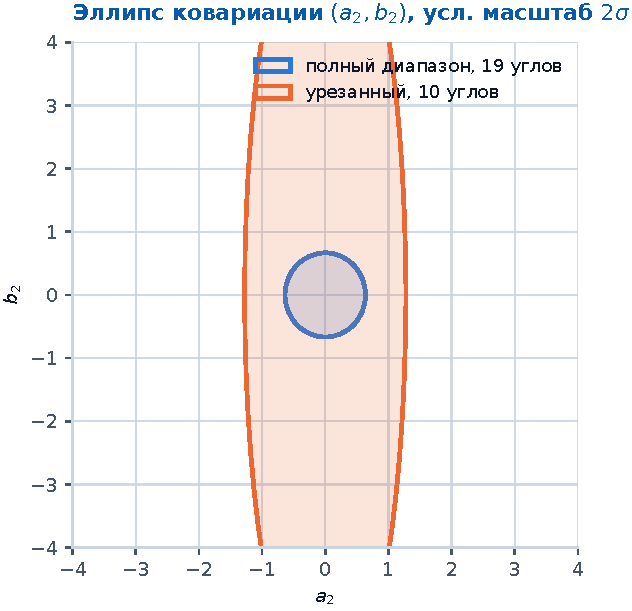
\includegraphics[width=0.82\linewidth]{figures/fig05_cov_ellipse.pdf}
  \caption{Эллипсы ковариации коэффициентов $(a_2,b_2)$ для двух планов таблицы
  примера~\ref{subsec:two-configs} (чистая геометрия $(X^{\mathsf T}X)^{-1}$ при единичном и
  одинаковом для всех точек шуме; масштаб эллипсов условный, важна их форма и вытянутость, а не
  абсолютный размер). Почти круглый эллипс полного диапазона против сильно вытянутого эллипса
  урезанного~--- то же число обусловленности, показанное геометрически.}
  \label{fig:cov-ellipse}
\end{figure}

% ---------------------------------------------------------------------
\subsection{Следствие: коллинеарность столбцов стоит вполне определённой цены}
\label{subsec:consequence}

Плохая обусловленность~--- не только про размер ошибки. У неё есть более коварное следствие:
если модель, применённая к плохо обусловленному плану, случайно \emph{забывает} один из
почти-коллинеарных столбцов (например, отбрасывает четвёртую гармонику, как это делает учебная
трёхпараметрическая форма §\ref{subsec:idea}), то оставшийся столбец вынужден скомпенсировать её
вклад~--- и оценка получает \term{систематическое смещение}, а не просто увеличенный разброс.

\begin{example}[: смещение офсета от одной лишь обрезки диапазона]\srckey{5.2}
На реальных развёртках сдвиг оценки офсета при переходе с полного диапазона на урезанный
составил:
\begin{center}
\footnotesize
\setlength{\tabcolsep}{7pt}
\begin{tabular}{@{}lr@{}}
\toprule
\textbf{Образец} & \textbf{Сдвиг $\theta_0$, полный $\to$ урезанный} \\
\midrule
плотная решётка, $D/P=0{,}71$        & $-0{,}687^\circ$ \\
повторная установка, $D/P=0{,}69$ (а) & $+0{,}351^\circ$ \\
повторная установка, $D/P=0{,}69$ (б) & $-2{,}103^\circ$ \\
разреженный образец, $D/P=0{,}46$    & $-0{,}920^\circ$ \\
\bottomrule
\end{tabular}
\end{center}
Величина сдвига~--- не шум измерения, а прямое следствие геометрии плана: она того же порядка,
что и обсуждаемые в проекте расхождения между конкурирующими оценками углового офсета,
полученными совсем другими методами. Иными словами, часть того, что могло бы показаться
содержательным физическим расхождением, оказывается артефактом одного лишь выбора углов
измерения.
\end{example}

\begin{warning}[: это не довод против урезанного диапазона как такового]
Урезанный диапазон~--- не ошибка сам по себе; в некоторых установках он вынужден геометрией
прибора. Проблема~--- не в его использовании, а в применении к нему модели, которая \emph{не
учитывает} все гармоники, необходимые для точного описания наблюдаемой (§\ref{subsec:idea}).
Если модель включает все пять коэффициентов, оценки остаются несмещёнными на любом диапазоне~---
меняется только их точность (столбец $\sigma(\theta_0)$ таблицы примера~\ref{subsec:two-configs}),
а не их центр.
\end{warning}

% ---------------------------------------------------------------------
\subsection{Мост к нелинейной задаче}
\label{subsec:bridge}

\begin{tcolorbox}[enhanced,colback=cS1!7,colframe=cS1,boxrule=0pt,leftrule=3pt,arc=1pt]
\textbf{Главная мысль параграфа, которая пригодится во всей оставшейся части курса.} Если два
столбца матрицы плана почти коллинеарны на множестве измеренных точек, соответствующие им
параметры \emph{почти неразличимы}: данные знают только их определённую комбинацию, а не каждый
параметр по отдельности. Это верно для линейной задачи, где всё считается в закрытой форме и
видно на эллипсе. В §§6--7 модель перестанет быть линейной по параметрам, замкнутой формулы для
ковариации больше не будет, и вместо матрицы плана~$X$ появится \term{якобиан} модели,
вычисленный в точке минимума. Но геометрический смысл~--- тот же самый: почти параллельные
столбцы якобиана означают почти неразличимые параметры. Именно этим механизмом в §9 объясняется
вырождение $\Deff\leftrightarrow\eta_0\leftrightarrow\varepsilon_{\rm cross}$~--- то же самое
явление, что в этом параграфе можно было увидеть глазом на эллипсе, просто в применении к
нелинейной модели, где эллипс уже не рисуется одной формулой.
\end{tcolorbox}

% ---------------------------------------------------------------------
\subsection{Типичные ошибки этого параграфа}

\begin{enumerate}[leftmargin=1.6em,itemsep=0.25em]
  \item Считать корреляцию параметров свойством \emph{данных} или метода подгонки. Она сидит в
        $(X^{\mathsf T}WX)^{-1}$, а $X$ строится только из углов измерения~--- корреляцию можно
        вычислить заранее, при планировании эксперимента.
  \item Путать увеличенную ошибку (разброс) со смещением (сдвигом центра оценки). Плохая
        обусловленность сама по себе даёт первое; смещение возникает только тогда, когда модель
        вдобавок отбрасывает один из почти-коллинеарных столбцов (§\ref{subsec:consequence}).
  \item Обрезать угловой диапазон и не пересмотреть при этом набор гармоник в модели. Урезанный
        диапазон не запрещён, но требует более осторожного отношения к тому, какие члены модели
        ещё различимы на нём.
  \item Считать, что вырождение параметров бывает только в нелинейных задачах. Это в первую
        очередь линейный эффект, который в линейной задаче виден напрямую~--- в нелинейной он
        просто прячется в якобиане (§\ref{subsec:bridge}).
\end{enumerate}

\clearpage
        % §5  Корреляция как свойство плана эксперимента
% % =====================================================================
%  §6. Лестница моделей и цена усложнения
%
%  ЖАНР (STYLE.md): учебная литература. Ни путей, ни имён программ, ни
%  номеров гипотез. Прослеживаемость — ключи \srckey{6.x} и приложение.
%
%  Содержательная основа: BRIEF_FOR_D_teaching_ladder.md §7; SYNTHESIS.md
%  §4, §7.1-7.3; опирается на теорему о выровненном анализаторе (§1).
% =====================================================================
\section{Лестница моделей и цена усложнения}
\label{sec:ladder}
\markboth{§\thesection. Лестница моделей}{}

К этому месту курс собрал целый набор возможных усложнений модели: конечная проводимость и
степенное рассеяние (§3), явное просачивание с собственной фазой (§1), комплексный перекрёстный
член, второй реальный элемент тракта вместо идеального анализатора (§1). Возникает практический
вопрос: в каком порядке их вводить, и как узнать, что усложнение того стоило? В этом параграфе
собран весь путь~--- от исходной геометрической модели §2 до модели, на которую опирается
дальнейшая часть курса,~--- и явно показана \term{цена} каждой ступени.

\begin{tcolorbox}[enhanced,colback=cPanel,colframe=cGrid,boxrule=0.8pt,arc=2pt,
                  title={\bfseries\color{cAccent} Пререквизиты},coltitle=cAccent,
                  attach boxed title to top left={xshift=6pt,yshift=-2pt},
                  boxed title style={colback=cPanel,boxrule=0pt,arc=0pt},top=10pt]
\textbf{Нужно знать:} §2 (геометрическая модель), §3 (Друде, степенные потери), §1 (просачивание,
теорема о выровненном анализаторе); понятие информационного критерия хотя бы на уровне «больше
параметров даёт лучший $\chi^2$ почти всегда, поэтому сравнивать модели по одному $\chi^2$
нечестно» (формальный вывод $\AIC=-2\ln L+2k$~--- в §8).\\[0.3em]
\textbf{Знать НЕ нужно:} вывод формулы AIC~--- в этом параграфе она используется как готовый
инструмент сравнения, обоснование появится в §8.
\end{tcolorbox}

% ---------------------------------------------------------------------
\subsection{Принцип: усложнение должно быть оплачено}
\label{subsec:pay-principle}

\begin{intuition}
Добавление любого нового свободного параметра почти никогда не ухудшает $\chi^2$ на тех же
данных, на которых модель обучена,~--- в худшем случае оптимизатор просто не воспользуется новой
свободой. Значит, сравнение моделей \emph{по одному лишь} $\chi^2$ всегда выберет более сложную
модель, даже если новый параметр не отражает никакой реальной физики. Нужна валюта, в которой
усложнение \emph{стоит} чего-то,~--- и такая валюта, штрафующая за каждый дополнительный
параметр,~--- информационный критерий Акаике.
\end{intuition}

\noindent
Практическое правило, которым пользуется этот параграф (полная шкала~--- в §8): изменение
$\dAIC$ порядка единиц означает «не различить»; порядка десятков~--- «уверенное улучшение»;
порядка тысяч~--- «прежняя модель категорически не годится».

% ---------------------------------------------------------------------
\subsection{Лестница для одного элемента тракта}
\label{subsec:ladder-single}

\begin{center}
\footnotesize
\setlength{\tabcolsep}{6pt}
\begin{tabular}{@{}p{0.14\linewidth}p{0.40\linewidth}p{0.40\linewidth}@{}}
\toprule
\textbf{Ступень} & \textbf{Что добавлено} & \textbf{Чем оплачено} \\
\midrule
базовая & чистая геометрическая модель §2 & точка отсчёта \\
$+$ материал & конечная проводимость (Друде) $+$ степенные потери §3 &
$\dAIC\approx-957$ (плотная решётка), $-266$ (разреженный образец)~--- уверенное улучшение на
обоих \\
$+$ свободный диаметр & $\Deff$ отпущен свободно, просачивание ещё не включено & здесь
возникает та самая загадка $\Deff/\Dphys$ из §\ref{sec:electrodynamics} \\
$+$ пин к физическому $D$, без просачивания & $\Deff$ приколочен к измеренному под микроскопом
диаметру & $\dAIC\approx+6167$~--- катастрофа: модель категорически хуже \\
$+$ явное просачивание & $\Deff$ приколочен к эффективному значению, добавлена
частотно-зависимая утечка $\eta(\nu)e^{\jj(\delta_0+2\pi\nu\tleak)}$ (§1) & \textbf{опорная
модель курса}: смещение в глубокой тени $3{,}38\to1{,}25$~дБ, среднеквадратичная ошибка
$2{,}21\to1{,}58$ \\
$+$ перекрёстный член & комплексная, не зависящая от угла добавка $\varepsilon_{\rm cross}$ &
улучшает $\AIC$, но не выдерживает проверку на нескольких образцах одновременно (ниже) \\
\bottomrule
\end{tabular}
\end{center}
\srckey{6.1}

\begin{warning}[: пин к физическому диаметру — не мелкая деталь, а диагностика]
Ступень «пин к физическому $D$» не улучшает модель, а \emph{ломает} её на $\dAIC$ порядка
тысяч~--- переоценивая тень на $7$--$10$~дБ. Это не значит, что физический диаметр измерен
неверно: это значит, что модель, в которую он подставлен, ещё не содержит канала, необходимого
для описания данных при физическом размере провода. Именно эта катастрофа~--- главный
экспериментальный аргумент за существование недостающего физического механизма, который
эффективный диаметр в предыдущих параграфах компенсировал сам (§\ref{sec:electrodynamics}).
\end{warning}

\begin{example}[: катастрофа воспроизводится не на одном образце]\srckey{6.2}
Провал пина к физическому диаметру без просачивания~--- не случайность одного набора измерений:
на трёх независимо измеренных образцах $\dAIC$ от такого пина составляет от нескольких тысяч до
$+9063$ на образце средней плотности. Универсальность провала~--- сильный довод в пользу того, что
недостающий канал общий для всех образцов, а не артефакт одной серии измерений.
\end{example}

% ---------------------------------------------------------------------
\begin{figure}[t]
  \centering
  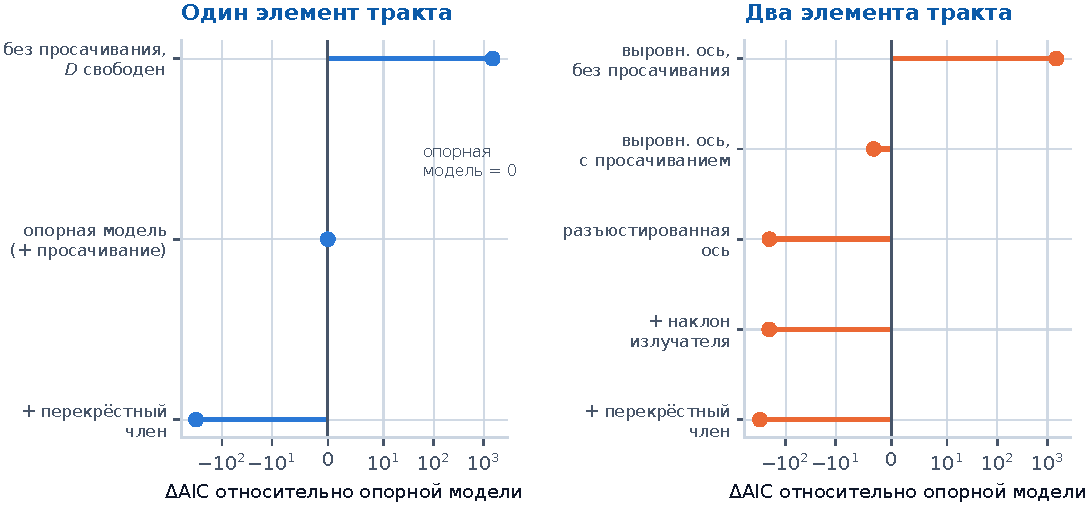
\includegraphics[width=\linewidth]{figures/fig06_ladder.pdf}
  \caption{Ступени лестницы для плотной решётки ($D/P=0{,}71$), информационный критерий
  относительно опорной модели курса. Слева~--- одиночный элемент тракта: от свободного диаметра
  без просачивания (наравне с его точным двух-элементным аналогом при выровненной оси, разница
  $0{,}15$~--- ключ~1.3) до опорной модели и её усложнения перекрёстным членом. Справа~--- та же
  лестница для двух реальных элементов тракта (§\ref{subsec:two-wgp}): пока ось выровнена,
  усложнение до второго реального элемента почти ничего не меняет; выигрыш появляется только
  вместе с разъюстировкой оси, которую отдельно обсуждает предупреждение
  §\ref{subsec:two-wgp}.}
  \label{fig:ladder}
\end{figure}

% ---------------------------------------------------------------------
\subsection{Перекрёстный член: улучшает подгонку, не проходит проверку}
\label{subsec:eps-cross}

Комплексный член $\varepsilon_{\rm cross}$, не зависящий от угла, улучшает согласие с данными на
отдельно взятом образце. Прежде чем принять его как физический эффект, естественно спросить:
одна ли это и та же константа тракта на разных образцах, или же подгонка каждый раз находит
удобное число под конкретный набор данных?

\begin{example}[: проверка на нескольких образцах отвергает гипотезу о константе тракта]\srckey{6.3}
Проверка однородности значения $\varepsilon_{\rm cross}$ между образцами отвергает гипотезу о
единой константе тракта: статистика проверки на однородность равна $761{,}6$ при $10$ степенях
свободы ($p=3{,}8\times10^{-157}$)~--- несовместимо со случайным разбросом вокруг одного истинного
значения. Отдельно, оценки просачивания образца и перекрёстного члена коррелируют между собой на
уровне $0{,}73$ (§1, ключ~1.2)~--- то есть параметр отчасти забирает на себя то, что должно было
бы принадлежать просачиванию.
\end{example}

\begin{intuition}[: как читать этот результат]
Улучшение $\AIC$ на одном образце говорит: «добавленный параметр помогает описать именно эти
данные». Проверка на нескольких образцах говорит нечто другое и более сильное: «помогает ли он
одним и тем же числом, как и должна вести себя константа тракта». Первое~--- необходимое условие
для физической интерпретации параметра, но не достаточное. Перекрёстный член проходит первую
проверку и не проходит вторую~--- значит, улучшение реально, а предложенная физическая
интерпретация (константа приёмного тракта) конкретно для этого параметра~--- нет.
\end{intuition}

% ---------------------------------------------------------------------
\subsection{Два элемента тракта: усложнение, которое не понадобилось}
\label{subsec:two-wgp}

Основная модель курса считает второй элемент тракта (анализатор перед приёмником) идеальным. Но
он~--- такой же реальный элемент, как исследуемый образец, со своим собственным просачиванием.
Соблазн очевиден: заменить идеальный анализатор его полной, реальной моделью и посмотреть, что
скажет подгонка. Это ровно та ситуация, для которой в §1 была доказана \term{теорема о
выровненном анализаторе}: если ось пропускания второго элемента совпадает с осью чувствительности
приёмника, его неидеальность \emph{ненаблюдаема}~--- она сводится к общему множителю, не
зависящему от угла.

\begin{strict}[: предсказание и его проверка (напоминание §1)]
Теорема предсказывает: явное включение второго реального элемента в модель не улучшит согласия
с данными и не сдвинет оценку эффективного диаметра. Измерено: изменение информационного критерия
$\dAIC=+0{,}15$ (усложнённая модель не лучше исходной~--- различие на два порядка меньше даже
самого скромного уверенного улучшения по шкале §\ref{subsec:pay-principle}), оценка эффективного
диаметра совпадает в четырёх значащих цифрах до и после усложнения.
\end{strict}

\begin{intuition}[: почему это ценный педагогический пример]
Модель усложнили честно~--- не отказались от идеи из осторожности, а реализовали её и запустили
подгонку,~--- и она отказалась усложняться ровно так, как было предсказано аналитически \emph{до}
расчёта. Отрицательный результат, полученный дважды (на бумаге и на данных),~--- такой же
полноценный научный результат, как и положительный: он экономит время, которое иначе ушло бы на
интерпретацию шума как физического эффекта.
\end{intuition}

\begin{warning}[: условие теоремы существенно, и с ним связана отдельная лестница]
Если ось второго элемента \emph{разъюстирована} относительно приёмника, условие теоремы
нарушается, и его неидеальность становится наблюдаемой. На данных это заметно: варианты модели,
явно учитывающие разъюстировку оси (и, отдельно, наклон излучателя), дают уверенное улучшение
$\AIC$ по сравнению с версией без такого учёта. Это не противоречит теореме~--- это именно то,
что она предсказывает при нарушении её условия,~--- но означает, что \emph{юстировка} тракта
имеет прямую количественную цену в качестве подгонки, тогда как \emph{полнота} модели анализатора
при аккуратной юстировке цены не имеет.
\end{warning}

% ---------------------------------------------------------------------
\subsection{Типичные ошибки этого параграфа}

\begin{enumerate}[leftmargin=1.6em,itemsep=0.25em]
  \item Сравнивать усложнённую и базовую модель по $\chi^2$ без штрафа за число параметров. Более
        сложная модель почти всегда даст $\chi^2$ не хуже~--- вопрос в том, оправдан ли выигрыш
        (§\ref{subsec:pay-principle}).
  \item Интерпретировать катастрофический $\dAIC$ пина к физическому диаметру как ошибку
        измерения диаметра. Это диагностика недостающего канала модели, а не претензия к
        микроскопии.
  \item Принять улучшение $\AIC$ на одном образце за доказательство физического смысла нового
        параметра. Нужна проверка на нескольких независимых образцах
        (§\ref{subsec:eps-cross})~--- она есть не всегда, и без неё вывод неполон.
  \item Усложнять модель «на всякий случай», не проверив заранее аналитически, не сводится ли
        усложнение к ненаблюдаемому множителю (§\ref{subsec:two-wgp}, теорема §1). Такая проверка
        стоит бумаги и карандаша и экономит недели вычислений.
  \item Спутать «юстировка не имеет значения» с «полнота модели анализатора не имеет значения».
        Верно второе при выполненном условии теоремы; первое неверно всегда.
\end{enumerate}

\clearpage
             % §6  Лестница моделей и цена усложнения
% % =====================================================================
%  §7. Нелинейный МНК: целевая функция, Левенберг–Марквардт, мультистарт
%
%  ЖАНР (STYLE.md): учебная литература. Ни путей, ни имён программ, ни
%  номеров гипотез. Прослеживаемость — ключи \srckey{7.x} и приложение.
%
%  Содержательная основа: BRIEF_FOR_D_teaching_ladder.md §8; SYNTHESIS.md.
% =====================================================================
\section{Нелинейный МНК: целевая функция, алгоритм, мультистарт}
\label{sec:nonlinear-fit}
\markboth{§\thesection. Нелинейный МНК}{}

Опорная модель курса (§6) содержит десяток параметров: геометрию, коэффициенты потерь, показатель
рассеяния, амплитуду и фазу просачивания, офсет угла. Ни один из них не входит в наблюдаемую
$U(\theta,\nu)$ линейно~--- диаметр стоит внутри логарифмов и рядов формулы Бланко (§2), показатель
рассеяния~--- в показателе степени (§3). Замкнутой формулы решения, какая была в §4, для такой
модели не существует. Этот параграф вводит инструментарий, без которого не обойтись при переходе
от линейной задачи к настоящей: каждое новое понятие появляется здесь как ответ на конкретную
неприятность, которая возникает, как только исчезает линейность.

\begin{tcolorbox}[enhanced,colback=cPanel,colframe=cGrid,boxrule=0.8pt,arc=2pt,
                  title={\bfseries\color{cAccent} Пререквизиты},coltitle=cAccent,
                  attach boxed title to top left={xshift=6pt,yshift=-2pt},
                  boxed title style={colback=cPanel,boxrule=0pt,arc=0pt},top=10pt]
\textbf{Нужно знать:} §4 (МНК, ковариация, веса) и §5 (корреляция, эллипс, обусловленность) как
образец того, что удаётся сделать в замкнутой форме; §6 (полный список параметров опорной
модели).\\[0.3em]
\textbf{Знать НЕ нужно:} вывод алгоритма Левенберга--Марквардта из первых принципов~--- здесь он
изложен на уровне интуиции, достаточном, чтобы понимать, что и почему может пойти не так.
\end{tcolorbox}

% ---------------------------------------------------------------------
\subsection{Целевая функция}
\label{subsec:objective}

За неимением замкнутого решения задача ставится явно: подобрать вектор параметров~$\mathbf{p}$,
минимизирующий взвешенную сумму квадратов невязок между моделью и измерением по всем углам и
частотам сразу:
\begin{equation}
  \mathbf{p}^\star=\argmin_{\mathbf{p}}\ \chi^2(\mathbf{p})
  =\argmin_{\mathbf{p}}\sum_{i}w_i\big[y_i-f(\mathbf{p};\theta_i,\nu_i)\big]^2 .
  \label{eq:objective}
\end{equation}
Формально это то же самое выражение, что и в §4~--- сумма взвешенных квадратов,~--- но $f$ теперь
нелинейна по~$\mathbf{p}$, и потому нормальные уравнения~\eqref{eq:normal-eq} перестают быть
линейной системой: производная $\partial\chi^2/\partial\mathbf{p}=0$ сама содержит~$\mathbf{p}$
нелинейно.

% ---------------------------------------------------------------------
\subsection{Веса амплитуды и фазы}
\label{subsec:weights-amp-phase}

Урок §\ref{subsec:weights} о весах здесь возвращается в усложнённом виде. Модель предсказывает не
только амплитуду сигнала, но и его фазу (§0, §1)~--- а амплитуда и фаза измеряются в разных
единицах и имеют разный динамический диапазон. Без отдельных весов для каждой из них одна
компонента невязки статистически подавляет другую~--- тот же эффект, что заглушение тени ярким
сигналом в §4, только теперь между двумя разнородными наблюдаемыми, а не между разными участками
одной и той же кривой. Решение~--- те же принципы, что в §4: взвешивать так, чтобы относительный
вклад каждой компоненты отражал её информативность, а не её случайный численный масштаб.

% ---------------------------------------------------------------------
\subsection{Маска динамического диапазона}
\label{subsec:mask}

\begin{warning}[: не весь диапазон данных одинаково надёжен]
В самой глубокой тени (углы, близкие к $90^\circ$) сигнал приближается к шумовому полу прибора:
там измеряется в основном шум, а не физика просачивания. Включение таких точек в подгонку с полным
весом добавляет в целевую функцию шум, который модель пытается <<объяснить>>, портя оценку
параметров, отвечающих именно за эту область.
\end{warning}

\noindent
Стандартное решение~--- \term{маска}: точки с отношением сигнал/шум ниже порога исключаются из
суммы~\eqref{eq:objective} или получают нулевой вес. Естественный вопрос: не превращается ли
результат затем в артефакт самой маски~--- не выбрасываем ли мы заодно и содержательный сигнал?

\begin{example}[: проверка того, что маска не создаёт эффект, а очищает его]\srckey{7.1}
Введение маски не ослабило, а \emph{усилило} свидетельство в пользу просачивания: улучшение
информационного критерия при добавлении явного просачивания выросло с $\dAIC\approx-533$ без
маски до $\dAIC\approx-657$ с ней. Если бы эффект был артефактом шума, маскирование шума должно
было бы его ослабить; произошло обратное~--- значит эффект не является порождением немаскированных
шумовых точек.
\end{example}

% ---------------------------------------------------------------------
\subsection{Алгоритм: гибрид спуска и метода Гаусса--Ньютона}
\label{subsec:lm}

\begin{intuition}
Вдали от минимума градиентный спуск надёжен, но медлителен: он делает маленькие осторожные шаги
вниз по склону. Вблизи минимума, где целевая функция похожа на параболу, метод
Гаусса--Ньютона сходится почти мгновенно, но вдали от минимума может <<перелететь>> или разойтись,
потому что опирается на локальную квадратичную аппроксимацию, верную только вблизи решения.
\term{Алгоритм Левенберга--Марквардта} плавно переключается между двумя стратегиями: параметр
затухания делает шаг похожим на осторожный градиентный спуск, когда прогресс плохой, и на быстрый
шаг Гаусса--Ньютона, когда прогресс хороший. Это стандартный рабочий инструмент нелинейного МНК
--- не единственный, но самый привычный выбор по умолчанию для задач такого размера.
\end{intuition}

% ---------------------------------------------------------------------
\begin{figure}[t]
  \centering
  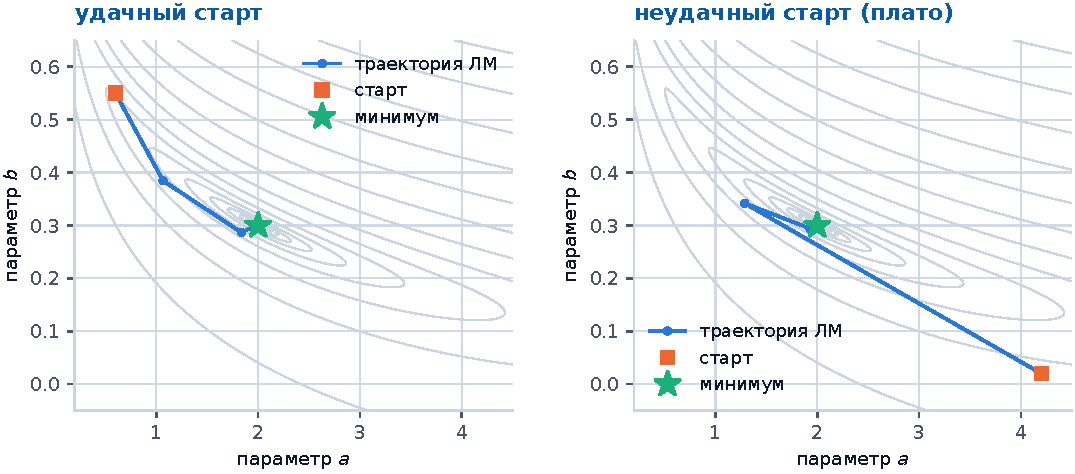
\includegraphics[width=0.86\linewidth]{figures/fig07_lm_trajectory.pdf}
  \caption{Иллюстрация алгоритма на учебной модельной задаче (не данные проекта): траектория
  Левенберга--Марквардта на линиях уровня целевой функции при удачном (сходится быстро) и
  неудачном (стартует в области, откуда путь к глобальному минимуму идёт через плоское плато)
  начальном приближении. Показана механика алгоритма, а не какой-либо из параметров опорной
  модели курса.}
  \label{fig:lm-trajectory}
\end{figure}

% ---------------------------------------------------------------------
\subsection{Начальное приближение перестаёт быть формальностью}
\label{subsec:init}

В линейной задаче §4 минимум был один, и стартовая точка не имела значения вообще~--- любое
решение линейной системы даёт один и тот же ответ. У нелинейной целевой функции может быть
\textbf{несколько локальных минимумов}, и алгоритм из §\ref{subsec:lm} находит ближайший к
стартовой точке, а вовсе не обязательно глобальный. Начальное приближение перестаёт быть
технической деталью и становится содержательным решением.

\begin{intuition}[: откуда берётся хороший старт почти бесплатно]
Гармонический разбор §4~--- решение линейной системы без итераций~--- сам по себе даёт оценки
офсета угла, амплитуды просачивания и относительной фазы каналов. Это не полная нелинейная
модель, но она даёт разумное первое приближение для соответствующих параметров нелинейной модели
почти без дополнительных затрат: \term{тёплый старт} из линейного разбора~--- стандартная практика,
которой стоит пользоваться всегда, когда она доступна.
\end{intuition}

% ---------------------------------------------------------------------
\subsection{Мультистарт и области притяжения}
\label{subsec:multistart}

\begin{warning}[: тёплый старт один — не гарантия]
Даже хороший тёплый старт не гарантирует сходимости к глобальному минимуму: у сложной модели
может быть несколько содержательно разных \term{областей притяжения}~--- множеств стартовых точек,
из которых алгоритм сходится к одному и тому же локальному решению,~--- и заранее не известно,
в какой из них попадёт конкретный старт.
\end{warning}

\begin{example}[: сколько стартов нужно на практике]\srckey{7.2}
На опорной модели курса из $21$ случайно выбранной стартовой точки в разных запусках получалось
от $3$ до $20$ различных областей притяжения (число зависело от конкретного набора данных и
параметризации), а доля стартов, попадающих в область глобального минимума, составила лишь
\textbf{$22{,}2\,\%$}. Решения из разных областей притяжения группировались по близости
информационного критерия (в пределах $0{,}5$ единиц $\AIC$), чтобы не считать одно и то же
решение, найденное с разной точностью сходимости, за <<разные>> результаты.
\end{example}

\begin{tcolorbox}[enhanced,colback=cS2!6,colframe=cS2,boxrule=0pt,leftrule=3pt,arc=1pt]
\textbf{История одной ошибки, которую стоит знать любому, кто планирует пользоваться нелинейным
МНК.} Раннее эмпирическое правило гласило: «тёплый старт лучше холодного, одного разумного старта
достаточно». Это правило пришлось \emph{отменить} после систематической проверки на сетке
стартов~--- выяснилось, что в глобальную область притяжения попадают лишь $22{,}2\,\%$ запусков, а
значит, единственный, пусть и разумный, старт даёт лишь вероятностный, а не гарантированный
результат.
\end{tcolorbox}

\begin{warning}[: конкретная цена одного старта — реальный отозванный результат]\srckey{7.3}
Значение перекрёстного члена $|\varepsilon_{\rm cross}|=0{,}0345$, ранее опубликованное по
результату одного старта, оказалось решением из \textbf{четвёртого} по качеству бассейна из
одиннадцати найденных~--- хуже глобального минимума на $192{,}5$ единиц информационного
критерия (шкала~--- §\ref{subsec:pay-principle}, «категорически хуже»). Число было отозвано,
как только сетка стартов вскрыла его происхождение. Здесь оно приводится единственный раз и
исключительно как иллюстрация того, к чему приводит доверие одному старту без проверки сеткой:
использовать его как физический результат~--- нельзя (полный список причин~--- в служебном
приложении курса).
\end{warning}

% ---------------------------------------------------------------------
\begin{figure}[t]
  \centering
  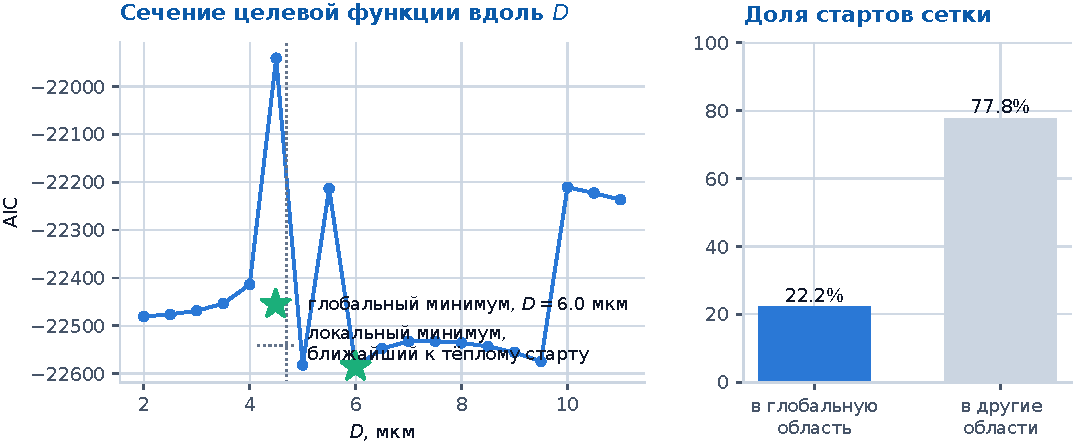
\includegraphics[width=\linewidth]{figures/fig07_basins.pdf}
  \caption{Слева: сечение целевой функции (информационный критерий) вдоль одного из параметров
  геометрии при фиксированных остальных~--- реальный расчёт, несколько локальных минимумов
  видны непосредственно на кривой; глобальный минимум отмечен отдельно, и он не совпадает с
  минимумом, ближайшим к границе физически правдоподобных значений. Справа: доля стартов,
  попадающих в область глобального минимума, по результатам сеточной проверки
  (§\ref{subsec:multistart}).}
  \label{fig:basins}
\end{figure}

% ---------------------------------------------------------------------
\subsection{Фиксация параметров при вырождении}
\label{subsec:pinning}

Когда два параметра почти неразличимы данными (§5 показал этот механизм в линейной задаче;
здесь он вернётся в §9 в полном объёме), свободная подгонка обоих~--- не консервативный, а
бессмысленный выбор: алгоритм найдёт какую-то комбинацию, устраивающую данные, но отчёты об
отдельных значениях будут вводить в заблуждение. Практический выход~--- \term{зафиксировать}
(«приколотить») один из вырожденных параметров на независимо обоснованном значении и подгонять
только второй. Так эффективный диаметр в опорной модели курса фиксируется не потому, что его
не пытались подгонять свободно, а потому, что свободная подгонка вместе с просачиванием даёт
не число, а признание собственной неопределённости, замаскированное под число (полный разбор~---
§9).

% ---------------------------------------------------------------------
\subsection{Ковариация без замкнутой формулы: бутстрап}
\label{subsec:bootstrap}

В линейной задаче §4 ковариация оценок была точной формулой. Для нелинейной модели стандартная
практика~--- приближённая ковариация вблизи минимума (обсуждается в §9) либо
\term{бутстрап}~--- многократное повторение подгонки на случайно пересемплированных версиях
данных, дающее эмпирическое распределение оценки.

\begin{warning}[: бутстрап требует независимости, а её нужно проверять, а не предполагать]\srckey{7.4}
Ресемплирование по отдельным точкам корректно только тогда, когда точки данных статистически
независимы. Пересемплирование \emph{по частотным отсчётам} на наших данных занижает ошибку в
$3{,}5$--$18{,}9$~раз, потому что соседние частотные точки коррелированы (одна и та же
физическая реализация шума и общий частотный профиль прибора размазаны по соседним отсчётам).
Ресемплирование должно происходить по единицам, которые \emph{действительно} независимы~---
например, по отдельным независимым измерениям, а не по каждой точке частотной сетки внутри
одного измерения.
\end{warning}

% ---------------------------------------------------------------------
\subsection{Типичные ошибки этого параграфа}

\begin{enumerate}[leftmargin=1.6em,itemsep=0.25em]
  \item Использовать один разумный (пусть и тёплый) старт и принимать результат как окончательный.
        Только сеточная проверка показывает, попал ли алгоритм в глобальную область притяжения
        (§\ref{subsec:multistart}).
  \item Расширять маску динамического диапазона, не проверив, усиливает или ослабляет она искомый
        эффект (§\ref{subsec:mask}) — иначе легко принять артефакт маскирования шума за
        содержательный результат, или наоборот, вычистить реальный эффект вместе с шумом.
  \item Свободно подгонять оба параметра из вырожденной пары «на всякий случай». Результат~---
        число, не несущее информации по отдельности (§\ref{subsec:pinning}, полный разбор~--- §9).
  \item Бутстрапировать по единицам данных, независимость которых не проверена. Соседние
        частотные отсчёты — типичный пример мнимой независимости (§\ref{subsec:bootstrap}).
  \item Забыть, что у Левенберга--Марквардта, как и у любого локального метода, нет встроенной
        гарантии глобальности~--- она появляется только вместе с мультистартом.
\end{enumerate}

\clearpage
      % §7  Нелинейный МНК: ЛМ, многостартовая оптимизация

% =====================================================================
%  ЧАСТЬ III. ДОСТОВЕРНОСТЬ: чему верить в полученных числах
% =====================================================================
% \part*{Часть III. Достоверность результата}
% \addcontentsline{toc}{section}{\textbf{Часть III. Достоверность результата}}

% % =====================================================================
%  §8. Правдоподобие, информационный критерий, анализ остатков
%
%  ЖАНР (STYLE.md): учебная литература. Ни путей, ни имён программ, ни
%  номеров гипотез. Прослеживаемость — ключи \srckey{8.x} и приложение.
%
%  Содержательная основа: BRIEF_FOR_D_teaching_ladder.md §9; SYNTHESIS.md §6.
% =====================================================================
\section{Правдоподобие, информационный критерий, анализ остатков}
\label{sec:likelihood}
\markboth{§\thesection. Правдоподобие и остатки}{}

Информационный критерий уже дважды использовался в курсе (§6~--- лестница моделей, §7~---
качество областей притяжения) как готовый инструмент со ссылкой «объяснение~--- в §8». Здесь
даётся обоснование: откуда вообще берётся штраф $2k$ и почему минимизация суммы квадратов~---
не техническая условность, а частный случай гораздо более общего принципа. Вторая половина
параграфа~--- то, что происходит \emph{после} подгонки: анализ остатков, обязательная, а не
факультативная часть работы, потому что хороший $\chi^2$ сам по себе ничего не говорит о том,
не остался ли в данных сигнал, который модель не объяснила.

\begin{tcolorbox}[enhanced,colback=cPanel,colframe=cGrid,boxrule=0.8pt,arc=2pt,
                  title={\bfseries\color{cAccent} Пререквизиты},coltitle=cAccent,
                  attach boxed title to top left={xshift=6pt,yshift=-2pt},
                  boxed title style={colback=cPanel,boxrule=0pt,arc=0pt},top=10pt]
\textbf{Нужно знать:} §6 (лестница моделей, качественная шкала $\dAIC$); §7 (целевая функция,
веса); нормальное распределение и его функция плотности.\\[0.3em]
\textbf{Знать НЕ нужно:} байесовский вывод информационных критериев~--- здесь используется
классический (частотный) вывод AIC Акаике, в его наиболее прикладной форме.
\end{tcolorbox}

% ---------------------------------------------------------------------
\subsection{От суммы квадратов к правдоподобию}
\label{subsec:likelihood}

\begin{strict}[: минимизация $\chi^2$ есть максимизация правдоподобия]
Пусть измерения $y_i$ отличаются от истинных значений модели $f(\mathbf{p};x_i)$ независимым
гауссовым шумом с известной дисперсией~$\sigma_i^2$. Плотность вероятности всего набора
измерений при данных параметрах~$\mathbf{p}$~--- \term{функция правдоподобия}:
\[
  L(\mathbf{p})=\prod_i\frac{1}{\sqrt{2\pi}\sigma_i}
  \exp\!\left[-\frac{(y_i-f(\mathbf{p};x_i))^2}{2\sigma_i^2}\right] .
\]
Её логарифм~--- сумма, а не произведение:
\[
  \ln L(\mathbf{p})=-\frac12\sum_i\frac{(y_i-f(\mathbf{p};x_i))^2}{\sigma_i^2}
  -\sum_i\ln(\sqrt{2\pi}\sigma_i)
  =-\tfrac12\chi^2(\mathbf{p})+\text{const} .
\]
Второе слагаемое от~$\mathbf{p}$ не зависит. Значит, тот параметр~$\mathbf{p}$, который
\emph{максимизирует} правдоподобие,~--- тот же самый, что \emph{минимизирует}~$\chi^2$ из
формулы~\eqref{eq:objective}. Взвешенный МНК всех предыдущих параграфов~--- не отдельный метод,
а максимизация правдоподобия в частном случае гауссова шума с весами $w_i=1/\sigma_i^2$.
\end{strict}

\begin{intuition}
Это не просто переобозначение. Как только подгонка признана максимизацией правдоподобия, к ней
становится применим весь аппарат статистического вывода, разработанный именно для правдоподобия,~---
в частности, сравнение моделей разной сложности, к которому курс и переходит.
\end{intuition}

% ---------------------------------------------------------------------
\subsection{Информационный критерий: плата за параметр}
\label{subsec:aic}

\begin{intuition}
Добавление любого нового параметра не может ухудшить максимум правдоподобия на тех же данных, на
которых модель обучена,~--- в худшем случае оптимизатор просто им не воспользуется. Сравнение
моделей по одному лишь $\ln L$ (или $\chi^2$) поэтому всегда предпочтёт более сложную модель, даже
если новый параметр не отражает никакой реальной структуры данных, а просто <<подстраивается>> под
шум. Нужна поправка, штрафующая за каждый дополнительный параметр,~--- она и называется
\term{информационным критерием Акаике}:
\begin{equation}
  \AIC=-2\ln L+2k,
  \label{eq:aic}
\end{equation}
где $k$~--- число свободных параметров модели. Из двух моделей предпочтительна та, у которой
$\AIC$ \emph{меньше}: она либо объясняет данные не хуже при меньшей сложности, либо оправдывает
дополнительную сложность реальным выигрышем в правдоподобии, превышающим штраф $2k$.
\end{intuition}

\noindent
Практическая шкала, уже использованная без обоснования в §6--§7 (общепринятая в статистической
литературе, число $10$~--- условный, но широко принятый порог):

\begin{center}
\footnotesize
\setlength{\tabcolsep}{8pt}
\begin{tabular}{@{}lp{0.62\linewidth}@{}}
\toprule
$|\dAIC|$ & \textbf{Что это означает} \\
\midrule
$\lesssim2$    & модели практически неразличимы данными \\
$2$--$10$      & умеренное свидетельство в пользу модели с меньшим $\AIC$ \\
$\gtrsim10$    & уверенное предпочтение \\
$\gtrsim$ сотни--тысячи & прежняя модель категорически не годится (пример~--- пин к физическому
диаметру, §6) \\
\bottomrule
\end{tabular}
\end{center}

\begin{warning}[: условие, без которого сравнение бессмысленно]
Формула~\eqref{eq:aic} сравнивает модели \emph{на одних и тех же данных}. Если у сравниваемых
вариантов разный набор точек, разные веса или разный способ построения предсказания, разность
$\AIC$ перестаёт что-либо означать~--- штраф $2k$ откалиброван на предположении, что единственное
отличие моделей~--- число параметров, а не подмена задачи. Вся лестница §6 построена так, что все
её ступени используют один и тот же набор точек и одни и те же веса именно по этой причине.
\end{warning}

% ---------------------------------------------------------------------
\subsection{Анализ остатков: обязательная проверка, а не украшение}
\label{subsec:residuals}

Хороший $\AIC$ говорит: «эта модель лучше той». Он не говорит: «эта модель исчерпала данные».
Ответ на второй вопрос даёт \term{остаток}~--- разность между измерением и предсказанием
наилучшей модели,~--- и то, насколько он похож на чистый шум.

\paragraph{Нормальность.} Если модель верна, а шум прибора гауссов, остаток должен быть похож на
выборку из нормального распределения. Стандартные проверки~--- критерии Шапиро--Уилка и
Жарка--Бера (числовые статистики) и \term{график квантиль-квантиль} (Q--Q): по оси абсцисс~---
квантили, которые дало бы точное нормальное распределение, по оси ординат~--- квантили реального
остатка. Если распределения совпадают, точки ложатся на прямую; систематическое отклонение от
прямой (особенно на хвостах) выдаёт структуру, которой в чистом шуме быть не должно.

\paragraph{Автокорреляция.} \term{Статистика Дарбина--Уотсона} измеряет корреляцию остатка с самим
собой, сдвинутым на один отсчёт: значение вблизи~$2$ означает отсутствие автокорреляции (белый
шум), значения, заметно меньшие двух, означают, что соседние точки остатка похожи друг на
друга~--- то есть в данных осталась \emph{структура}, которую модель не объяснила, а не случайный
разброс.

\begin{example}[: две крайности одного проекта]\srckey{8.1}
На плотной решётке после включения всех поправок опорной модели (§6) статистика
Дарбина--Уотсона остатка по амплитуде составляет $\approx0{,}32$~--- далеко от идеала~$2$: остаток
всё ещё заметно структурен, модель не полна. На разреженном образце та же статистика после той же
модели даёт $\approx1{,}76$~--- почти белый шум: там модель практически исчерпала данные. Одна и
та же модель, применённая к двум образцам, оставляет принципиально разное количество необъяснённой
структуры~--- сам факт этого различия является диагностикой не хуже, чем абсолютное значение.
\end{example}

% ---------------------------------------------------------------------
\begin{figure}[t]
  \centering
  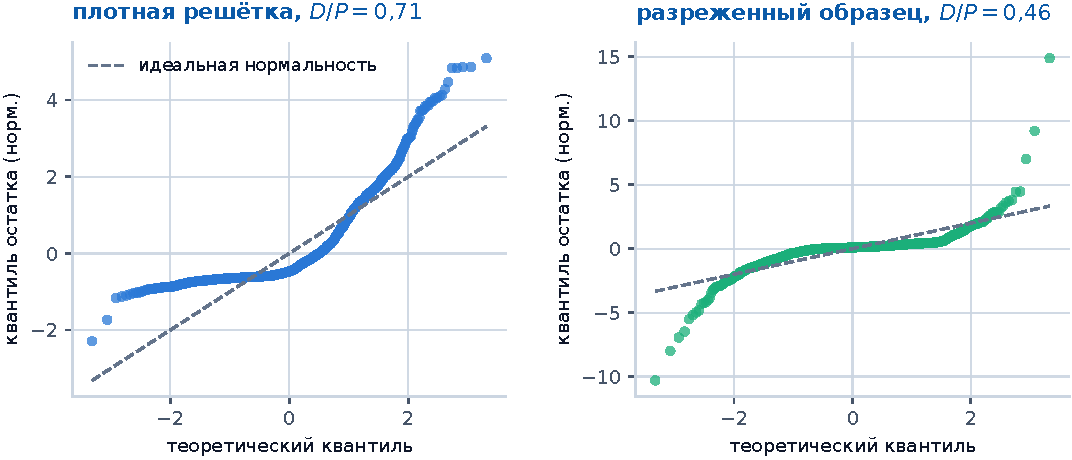
\includegraphics[width=\linewidth]{figures/fig08_qq.pdf}
  \caption{График квантиль-квантиль остатка амплитуды (плотная решётка против разреженного
  образца, модель без явного просачивания~--- тот же срез, на котором была впервые замечена
  структура остатка, обсуждаемая ниже). Прямая линия отвечала бы точной нормальности;
  систематическое искривление на краях, заметно более выраженное для плотной решётки, выдаёт
  негауссовость остатка.}
  \label{fig:qq}
\end{figure}

\paragraph{Карты остатков.} Если остаток зависит и от угла, и от частоты, полезно смотреть не на
одномерные срезы, а на двумерную карту угол\,$\times$\,частота: локализованное <<пятно>> отклонения
подсказывает физический механизм гораздо точнее, чем усреднённая по всем точкам статистика.

\begin{example}[: так был найден дефицит тени]\srckey{8.2}
Именно карта остатков угол\,$\times$\,частота, построенная для модели без явного просачивания,
впервые локализовала систематическую недооценку сигнала в глубокой тени~--- порядка $3$--$4$~дБ, и
только на плотном образце, а не разреженном. Это наблюдение и стало отправной точкой для введения
явного просачивания в §1 и §6: карта остатков не просто зафиксировала, что модель <<не идеальна>>,
а указала, \emph{где именно} и \emph{насколько}, что резко сузило круг гипотез.
\end{example}

\begin{figure}[t]
  \centering
  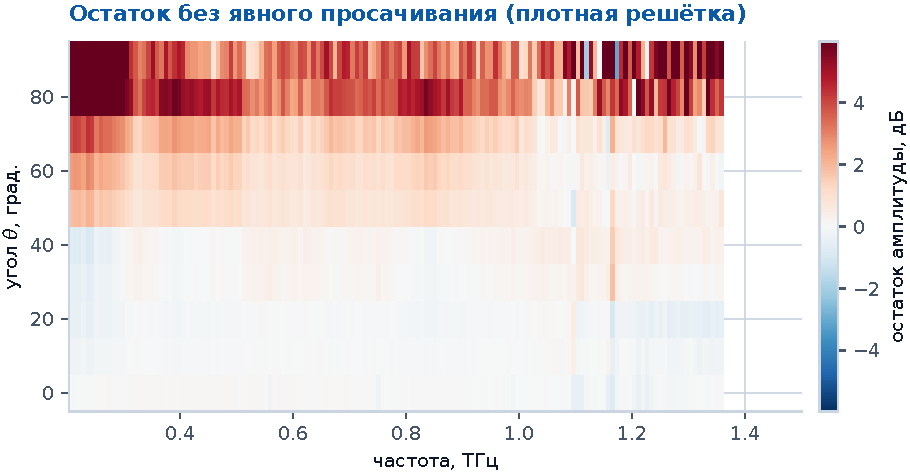
\includegraphics[width=\linewidth]{figures/fig08_residual_map.pdf}
  \caption{Карта остатка амплитуды (угол против частоты) для плотной решётки, модель без явного
  просачивания. Систематическое усиление отклонения к большим углам~--- то самое наблюдение,
  которое привело к введению просачивания в опорную модель курса (§1, §6).}
  \label{fig:residual-map}
\end{figure}

\paragraph{Разложение остатка по осям.} После того как явное просачивание уже включено в модель
(§6), остаток на плотном образце всё ещё содержит два опознаваемых компонента: локализованный
<<горячий>> пик на низкой частоте (около $0{,}21$--$0{,}22$~ТГц, амплитуда порядка $1{,}7$--$1{,}8$~дБ)
и гладкий дисперсионный наклон около $-0{,}62$~дБ на терагерц по всей полосе. Ни то, ни другое
пока не отнесено к конкретному физическому механизму с уверенностью~--- это открытый остаток,
честно предъявленный, а не спрятанный.\srckey{8.3}

\paragraph{Проверка на отложенных данных (held-out).} Самая строгая проверка~--- не то, насколько
хорошо модель описывает те же данные, на которых обучена, а то, переносится ли параметр,
измеренный на одной части данных, на другую. Просачивание, оценённое по яркой части развёртки
(там, где сигнал велик и шум относительно мал), можно проверить, подставив его в предсказание для
тени~--- части данных, не участвовавшей в этой оценке.

\begin{example}[: хороший фит — не то же самое, что предсказательная сила]\srckey{8.4}
Параметр амплитуды просачивания, определённый по ярким углам, даёт среднеквадратичную ошибку
$0{,}50$~дБ на самих ярких углах, но $3{,}75$~дБ при попытке предсказать глубокую тень~---
почти в восемь раз хуже. Мораль: способность модели хорошо описать те данные, по которым
оценивался параметр,~--- необходимое, но не достаточное условие того, что параметр физически верно
характеризует весь диапазон измерения.
\end{example}

% ---------------------------------------------------------------------
\subsection{Различение, ради которого всё это делается}
\label{subsec:distinction}

\begin{tcolorbox}[enhanced,colback=cS1!7,colframe=cS1,boxrule=0pt,leftrule=3pt,arc=1pt]
\textbf{«Модель лучше описывает данные» и «параметр модели измерен» — разные утверждения.} Курс
уже трижды сталкивался с этим различением по частям: показатель рассеяния~$\gamma$ (§3)~---
эффект реален, конкретное значение плывёт в разы в зависимости от соседних членов модели;
перекрёстный член (§6)~--- улучшает $\AIC$ на одном образце, не проходит проверку однородности
между образцами; амплитуда просачивания (только что, §\ref{subsec:residuals})~--- хорошо описывает
те данные, по которым получена, но не экстраполируется. §9 соберёт это различение в общий
формальный аппарат~--- информацию Фишера и профильное правдоподобие,~--- которым можно проверять
его заранее, не дожидаясь held-out теста по факту.
\end{tcolorbox}

% ---------------------------------------------------------------------
\subsection{Типичные ошибки этого параграфа}

\begin{enumerate}[leftmargin=1.6em,itemsep=0.25em]
  \item Сравнивать модели по $\AIC$, посчитанному на разных наборах точек или с разными весами.
        Штраф $2k$ откалиброван на предположении, что данные и способ их взвешивания общие
        (§\ref{subsec:aic}).
  \item Считать хороший $\chi^2$ или $\AIC$ достаточным основанием не смотреть на остатки. Модель
        может быть <<лучшей из предложенных>> и одновременно далёкой от исчерпания данных
        (пример со статистикой Дарбина--Уотсона, §\ref{subsec:residuals}).
  \item Усреднять остаток по одной из осей (только по углу или только по частоте) прежде, чем
        проверить двумерную карту. Локализованный дефект легко потерять при усреднении.
  \item Считать, что параметр, хорошо описывающий обучающую часть данных, автоматически годится
        для экстраполяции. Held-out проверка~--- отдельный и более строгий тест
        (§\ref{subsec:residuals}).
  \item Путать «эффект статистически значим» с «параметр физически измерен»~--- это ровно то
        различение, ради которого написан весь параграф (§\ref{subsec:distinction}).
\end{enumerate}

\clearpage
         % §8  Правдоподобие, AIC и анализ остатков
% % =====================================================================
%  §9. Идентифицируемость: Фишер, вырождение, профиль, бутстрап
%
%  ЖАНР (STYLE.md): учебная литература. Ни путей, ни имён программ, ни
%  номеров гипотез. Прослеживаемость — ключи \srckey{9.x} и приложение.
%
%  Содержательная основа: BRIEF_FOR_D_teaching_ladder.md §1, §8;
%  SYNTHESIS.md §3, §8.
% =====================================================================
\section{Идентифицируемость: вырождение, профиль, бутстрап}
\label{sec:identifiability}
\markboth{§\thesection. Идентифицируемость}{}

§5 показал на линейной задаче: если два столбца матрицы плана почти коллинеарны, соответствующие
параметры почти неразличимы, и это видно на эллипсе ковариации напрямую. §7 упомянул, что для
нелинейной модели та же болезнь существует, только матрица плана заменяется якобианом в точке
минимума, а эллипс~--- уже не рисуется одной формулой. Здесь этот обещанный переход выполняется до
конца: вводится формальный аппарат (информация Фишера), разбирается конкретное, самое
чувствительное вырождение опорной модели курса, и показывается, почему в вырожденном случае
привычная параболическая оценка ошибки откровенно врёт.

\begin{tcolorbox}[enhanced,colback=cPanel,colframe=cGrid,boxrule=0.8pt,arc=2pt,
                  title={\bfseries\color{cAccent} Пререквизиты},coltitle=cAccent,
                  attach boxed title to top left={xshift=6pt,yshift=-2pt},
                  boxed title style={colback=cPanel,boxrule=0pt,arc=0pt},top=10pt]
\textbf{Нужно знать:} §5 целиком (обусловленность, эллипс ковариации); §7 (целевая функция,
фиксация параметров, бутстрап); §8 (правдоподобие, $\AIC$).\\[0.3em]
\textbf{Знать НЕ нужно:} общую байесовскую теорию идентифицируемости моделей~--- здесь всё
разбирается на одном конкретном, уже знакомом курсу примере.
\end{tcolorbox}

% ---------------------------------------------------------------------
\subsection{Информация Фишера: якобиан вместо матрицы плана}
\label{subsec:fisher}

\begin{strict}
Вблизи максимума правдоподобия (минимума $\chi^2$) логарифм правдоподобия хорошо приближается
параболой, и \term{матрица информации Фишера} играет роль, которую в §5 играла $X^{\mathsf T}WX$:
\begin{equation}
  \mathcal{I}(\mathbf{p}^\star)\approx J^{\mathsf T}WJ,
  \qquad
  J_{i\alpha}=\frac{\partial f(\mathbf{p};x_i)}{\partial p_\alpha}\bigg|_{\mathbf{p}^\star},
  \qquad
  \operatorname{Cov}(\mathbf{p}^\star)\approx\mathcal{I}^{-1} .
  \label{eq:fisher}
\end{equation}
Это тот же самый алгоритм Гаусса--Ньютона, что стоит внутри Левенберга--Марквардта (§7): якобиан
$J$~--- линеаризация нелинейной модели \emph{в точке минимума}. Вся геометрия §5 (эллипсы,
обусловленность, почти коллинеарные столбцы) переносится сюда без изменений~--- меняется только
то, что раньше $X$ была задана планом заранее, а теперь $J$ вычисляется в конкретной, уже
найденной точке и, вообще говоря, меняется от точки к точке.
\end{strict}

\begin{intuition}[: что означают собственные числа $\mathcal{I}$]
Разложение $\mathcal{I}$ по собственным векторам делит пространство параметров на
\term{хорошо определённые} направления (большое собственное число~--- узкое направление
эллипсоида, данные сильно ограничивают соответствующую комбинацию параметров) и
\term{плохо определённые} (маленькое собственное число~--- широкое направление, вдоль него данные
почти ничего не говорят). Как правило, эти направления~--- не отдельные параметры модели, а их
\emph{комбинации}: данные хорошо знают одну линейную (или нелинейную) смесь параметров и почти
ничего не знают об ортогональной ей смеси.
\end{intuition}

% ---------------------------------------------------------------------
\subsection{Конкретное вырождение опорной модели}
\label{subsec:degeneracy}

Самое чувствительное направление опорной модели курса связывает три параметра: эффективный
диаметр $\Deff$ (§\ref{sec:electrodynamics}, §6), амплитуду просачивания~$\eta_0$ (§1, §6) и
перекрёстный член~$\varepsilon_{\rm cross}$ (§6).

\begin{example}[: насколько сильно вырождены $\Deff$ и $\eta_0$]\srckey{9.1}
Корреляция оценок $\Deff$ и~$\eta_0$ при их совместной свободной подгонке составляет
$-0{,}999999$~--- по сути, минус единица. Соответствующая пара параметров ведёт себя не как два
независимых числа, а как одна степень свободы: данные знают некоторую их комбинацию (условно,
<<общий дефицит канала подавления>>) практически точно, а способ, которым эта комбинация делится
между <<геометрией>> и <<просачиванием>>,~--- почти произвольно.
\end{example}

\begin{warning}[: что происходит, если подгонять оба параметра свободно]\srckey{9.2}
Свободная совместная подгонка $\Deff$ на плотной решётке даёт $1{,}85\pm8{,}37$~мкм. Формально
это число с оценкой ошибки; по существу~--- признание того, что данные почти ничего не говорят об
этом параметре по отдельности, замаскированное под результат измерения. Ошибка $8{,}37$~мкм
превышает само центральное значение более чем вчетверо~--- уже этого достаточно, чтобы
заподозрить вырождение прежде, чем разбираться в его происхождении.
\end{warning}

% ---------------------------------------------------------------------
\subsection{Профильное правдоподобие: когда параболическая ошибка врёт}
\label{subsec:profile}

Оценка ошибки из формулы~\eqref{eq:fisher} предполагает, что $\chi^2$ вблизи минимума~---
парабола. Это предположение стоит проверять, а не принимать по умолчанию~--- особенно рядом с
вырождением. \term{Профильное правдоподобие} строится так: параметр (здесь~--- $\Deff$)
поочерёдно фиксируется на серии значений, а на каждом шаге \emph{все остальные} параметры
подгоняются заново. Получается кривая «лучший $\chi^2$ (или $\AIC$) при данном фиксированном
значении $\Deff$» — честная картина того, что данные на самом деле знают об этом параметре, без
предположения о параболичности.

\begin{example}[: профиль не параболичен и не совпадает со свободной оценкой]\srckey{9.3}
Профиль $\AIC(\Deff)$ на плотной решётке имеет глобальный минимум около $\Deff\approx6$~мкм~---
заметно отличается от свободной оценки $1{,}85$~мкм из §\ref{subsec:degeneracy}, и по пути к нему
$\AIC$ ведёт себя не монотонно: есть промежуточные локальные минимумы разной глубины, а не одна
гладкая парабола. Мера «уплощённости» профиля (отношение размаха $\AIC$ на профиле к его
типичному шагу) далека от той, что была бы у чистой параболы. Свободная нелинейная подгонка,
предоставленная себе, не обязана найти этот более глубокий минимум~--- в этом состоит прямая связь
с многостартовой оптимизацией §7: то же самое вырождение, которое портит параболическую оценку
ошибки, одновременно создаёт дополнительные локальные минимумы для алгоритма подгонки.
\end{example}

\begin{figure}[t]
  \centering
  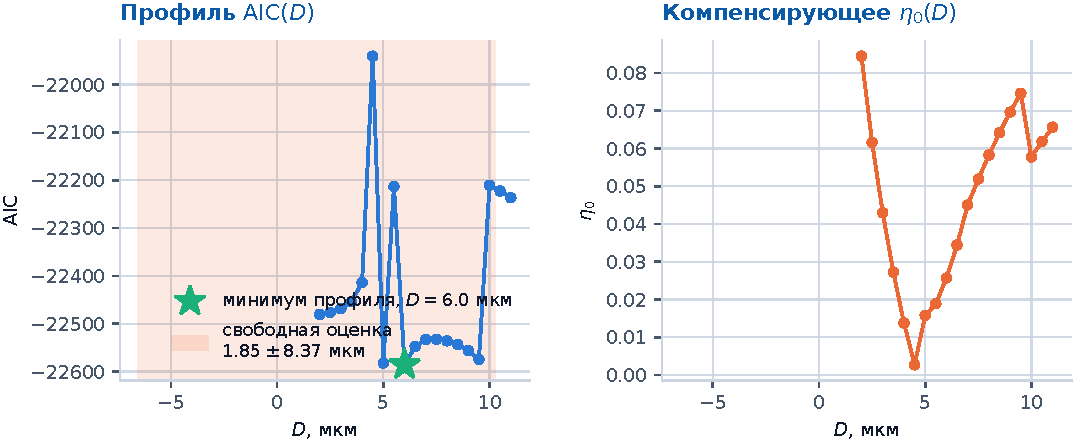
\includegraphics[width=\linewidth]{figures/fig09_profile.pdf}
  \caption{Слева: профиль $\AIC(\Deff)$ (та же кривая, что уже приводилась в §7 как иллюстрация
  множественных локальных минимумов, здесь~--- в контексте идентифицируемости). Справа: та же
  сетка значений $\Deff$, но по оси ординат~--- значение $\eta_0$, на которое переоптимизируются
  остальные параметры при каждом фиксированном $\Deff$: видно почти линейное компенсирующее
  движение~--- прямое графическое проявление вырождения, дополняющее число корреляции
  примера~\ref{subsec:degeneracy}.}
  \label{fig:profile}
\end{figure}

\begin{intuition}[: почему это не противоречие, а согласованная картина]
Свободная подгонка $1{,}85\pm8{,}37$~мкм и профильный минимум $6$~мкм не спорят друг с другом~---
они говорят одно и то же на разных языках. Огромная параболическая ошибка~--- симптом того, что
локальная (гауссова) аппроксимация вблизи найденной алгоритмом точки не годится глобально; профиль
честно показывает, что <<настоящий>> минимум может быть в стороне и не быть параболическим.
Обе картины согласны в главном: $\Deff$, оценённый свободно вместе с $\eta_0$, не является
надёжно измеренным числом.
\end{intuition}

% ---------------------------------------------------------------------
\subsection{Карта корреляций: с чем ещё конкурирует диаметр}
\label{subsec:corrmap}

Вырождение $\Deff\leftrightarrow\eta_0$~--- самое сильное, но не единственное. Полная карта
корреляций диаметра со всеми остальными параметрами опорной модели показывает, что диаметр
практически неотделим (корреляция по модулю $\gtrsim0{,}99$) от целой группы параметров,
отвечающих за амплитуду и фазу просачивания, и гораздо слабее связан с параметрами материала
(показатель рассеяния, коэффициент потерь) и офсетом угла.

\begin{figure}[t]
  \centering
  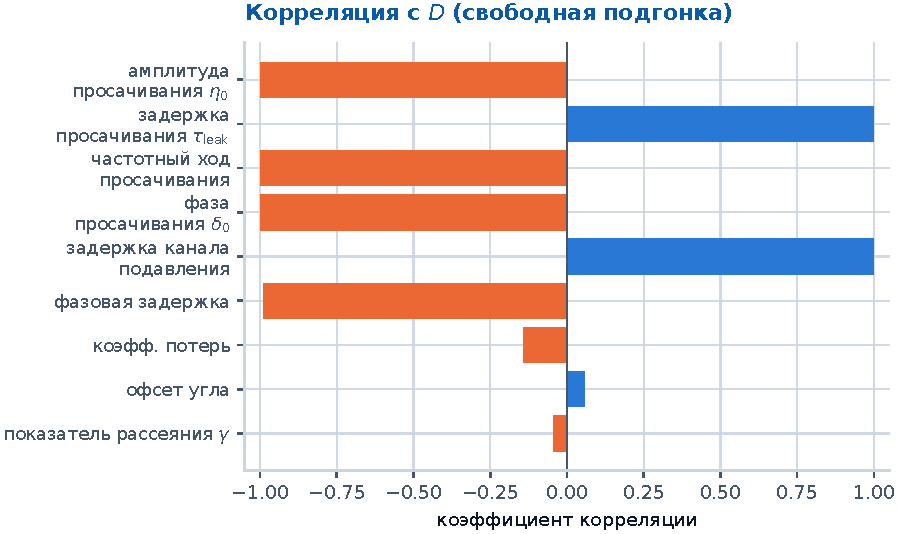
\includegraphics[width=0.82\linewidth]{figures/fig09_corrmap.pdf}
  \caption{Корреляция свободной оценки $\Deff$ со всеми остальными параметрами опорной модели при
  совместной подгонке (плотная решётка). Группа параметров просачивания практически неотличима от
  диаметра по модулю корреляции; параметры материала связаны с ним значительно слабее.}
  \label{fig:corrmap}
\end{figure}

\begin{intuition}[: практический вывод из формы карты]
Карта корреляций~--- готовый рецепт того, \emph{что именно} стоит фиксировать, а что можно
оставлять свободным. Параметр, слабо коррелирующий с диаметром (например, показатель рассеяния),
можно уверенно подгонять одновременно с ним. Параметр из группы с корреляцией, близкой к
единице, подгонять одновременно с диаметром бессмысленно~--- нужно зафиксировать один из пары на
независимо обоснованном значении, как это было сделано в §6--§7.
\end{intuition}

% ---------------------------------------------------------------------
\subsection{Бутстрап при вырождении: не эллипс, а «банан»}
\label{subsec:bootstrap-degenerate}

§7 предупреждал: бутстрап требует независимости пересемплируемых единиц. При вырождении
добавляется вторая ловушка, уже не про независимость данных, а про форму результата.

\begin{warning}[: линейная ошибка описывает вырождение только локально]
Формула~\eqref{eq:fisher} и эллипс ковариации~--- это локальное, линеаризованное описание. Когда
данные ограничивают не сам параметр, а нелинейную комбинацию нескольких параметров (как в
§\ref{subsec:degeneracy}), облако точек бутстрапа~--- повторных подгонок на пересемплированных
данных~--- часто вытягивается не в эллипс, а в изогнутую, «банановидную» полосу вдоль поверхности
уровня вырождения. Сообщать в этом случае только пару чисел (центр и симметричная ошибка)~---
терять как раз ту информацию о форме, ради которой бутстрап обычно и делают.
\end{warning}

\begin{intuition}[: как читать такой результат честно]
Правильный вывод из «банановидного» бутстрапа~--- не «параметр измерен плохо», а «данные измеряют
не этот параметр, а некоторую его комбинацию с соседним, и вот форма этой комбинации». Это
содержательный физический вывод, просто не в форме «значение $\pm$ ошибка», к которой хочется
свести любой результат.
\end{intuition}

% ---------------------------------------------------------------------
\subsection{Практический вывод: что и почему фиксировать}
\label{subsec:conclusion}

\begin{tcolorbox}[enhanced,colback=cS1!7,colframe=cS1,boxrule=0pt,leftrule=3pt,arc=1pt]
Собранный в этом параграфе аппарат объясняет решение, принятое ещё в §6--§7 без полного
обоснования: почему эффективный диаметр в опорной модели курса \term{фиксируется}, а не
подгоняется свободно. Свободная подгонка вместе с просачиванием измеряет не $\Deff$ и не
$\eta_0$ по отдельности, а их почти неразличимую комбинацию (§\ref{subsec:degeneracy}), причём
параболическая оценка ошибки в этой точке систематически вводит в заблуждение
(§\ref{subsec:profile}). Фиксация одного из вырожденной пары на независимо обоснованном значении
(например, физическом диаметре, где он доступен,~--- хотя, как показал §6, именно этот выбор
катастрофичен для качества подгонки, что само по себе физический результат) — единственный
способ получить осмысленную, а не иллюзорную оценку второго параметра.
\end{tcolorbox}

% ---------------------------------------------------------------------
\subsection{Типичные ошибки этого параграфа}

\begin{enumerate}[leftmargin=1.6em,itemsep=0.25em]
  \item Доверять параболической (фишеровской) оценке ошибки без проверки профильным
        правдоподобием, особенно вблизи известного или подозреваемого вырождения
        (§\ref{subsec:profile}).
  \item Интерпретировать огромную ошибку свободной оценки как «неточное измерение», а не как
        симптом вырождения, требующий фиксации одного из параметров.
  \item Сообщать результат бутстрапа при вырождении только как «значение $\pm$ ошибка», теряя
        форму облака точек, которая часто содержит больше физики, чем два числа
        (§\ref{subsec:bootstrap-degenerate}).
  \item Фиксировать параметр «для определённости», не проверив по карте корреляций, действительно
        ли он входит в сильно вырожденную группу (§\ref{subsec:corrmap}).
  \item Забыть, что вырождение~--- не патология конкретной подгонки, а прямое следствие
        ограниченного числа независимых чисел в измерении, о котором курс говорил ещё в §0 и §5:
        оно не лечится ни лучшим алгоритмом, ни большим числом итераций.
\end{enumerate}

\clearpage
    % §9  Идентифицируемость, вырождение, Фишер, профиль
% % =====================================================================
%  §10. Метод анализа: рабочие правила с кейсами
%
%  ЖАНР (STYLE.md): учебная литература. Ни путей, ни имён программ, ни
%  номеров гипотез. Прослеживаемость — ключи \srckey{10.x} и приложение.
%
%  Содержательная основа: BRIEF_FOR_D_teaching_ladder.md §10.
% =====================================================================
\section{Метод анализа: рабочие правила с кейсами}
\label{sec:method}
\markboth{§\thesection. Метод анализа}{}

Части~I--III дали физику, аппарат оценивания и аппарат проверки достоверности. Этот заключительный
параграф~--- не новая математика, а свод из девяти рабочих правил, по которым строилось всё
предыдущее изложение. Каждое правило сформулировано абстрактно и сразу же проиллюстрировано
конкретным случаем из того же проекта, на данных которого построен весь курс~--- так, чтобы правило
запоминалось не как лозунг, а как приём с понятной ценой ошибки, если им пренебречь.

\begin{tcolorbox}[enhanced,colback=cPanel,colframe=cGrid,boxrule=0.8pt,arc=2pt,
                  title={\bfseries\color{cAccent} Пререквизиты},coltitle=cAccent,
                  attach boxed title to top left={xshift=6pt,yshift=-2pt},
                  boxed title style={colback=cPanel,boxrule=0pt,arc=0pt},top=10pt]
\textbf{Нужно знать:} весь курс, §0--§9~--- каждое правило опирается на аппарат и примеры,
введённые ранее, и явно на них ссылается.\\[0.3em]
\textbf{Знать НЕ нужно:} ничего нового~--- этот параграф собирает уже известное в рабочий
чек-лист.
\end{tcolorbox}

% ---------------------------------------------------------------------
\subsection{1. Модельно-независимое прежде модельного}
\label{subsec:rule1}

Прежде чем доверять выводу, полученному подгонкой сложной модели, стоит спросить: можно ли
установить тот же факт способом, не зависящим от правоты модели вообще,~--- симметрией,
периодичностью, законом сохранения энергии?

\begin{example}[: расхождение объяснено ещё до всякой подгонки]\srckey{10.1}
На одном из образцов повторные измерения, снятые в разные дни, расходились в области глубокого
подавления почти в полтора раза. Причина была установлена \emph{без единого фита}: угол $-95^\circ$
физически задаёт ту же ориентацию проводов, что и $+85^\circ$ (поляризатор не различает
направление вращения на $180^\circ$~--- §\ref{sec:electrodynamics}), а измерения в двух
конфигурациях эту симметрию не учитывали одинаково. Модельная подгонка, проведённая позже,
только подтвердила уже установленный факт.
\end{example}

% ---------------------------------------------------------------------
\subsection{2. Отрицательный контроль обязателен}
\label{subsec:rule2}

Эффект, добавленный в модель, стоит проверять не только там, где он предположительно есть, но и
там, где, по своей же физике, его быть не должно. Если он «находится» одинаково хорошо
и в контрольных условиях, подозрение падает на метод, а не на физику.

\begin{example}[: просачивание проходит контроль честно]\srckey{10.2}
Явное просачивание нужно плотной решётке (уверенное улучшение $\AIC$, §6) и \emph{не нужно}
разреженному образцу: там амплитуда просачивания стремится к нулю, а добавление параметра лишь
штрафует $\AIC$ без всякого выигрыша. Это ровно то поведение, которого требует отрицательный
контроль,~--- эффект, «находимый» одинаково везде независимо от физических условий, как правило,
оказывается артефактом метода, а не реальностью.
\end{example}

% ---------------------------------------------------------------------
\subsection{3. Предсказание фиксируется до расчёта}
\label{subsec:rule3}

Самая убедительная проверка гипотезы~--- не подгонка задним числом, а численное предсказание,
сделанное \emph{на бумаге}, до того как получен результат расчёта или измерения.

\begin{example}[: теорема, а не апостериорное объяснение]\srckey{10.3}
Теорема о выровненном анализаторе (§1) предсказала конкретное число~--- изменение информационного
критерия, близкое к нулю,~--- \emph{до} того, как модель со вторым реальным элементом тракта была
запущена. Измерено $\dAIC=+0{,}15$ (§1, §6): предсказание подтвердилось количественно, а не
только по знаку. Такая проверка гораздо строже, чем подбор объяснения под уже известный результат.
\end{example}

% ---------------------------------------------------------------------
\subsection{4. Триангуляция}
\label{subsec:rule4}

Один путь к результату~--- гипотеза. Два и более независимых пути, сходящихся к одному и тому же
числу,~--- уже результат, которому можно доверять существенно больше.

\begin{example}[: просачивание подтверждено тремя разными способами]\srckey{10.4}
Существование и величина просачивания подтверждены: (а) явным включением его в подгонку
(§6); (б) энергетическим балансом развёртки без всякой подгонки спектра, по формуле~$\cos^4\theta$
из §0; (в) прямым наблюдением временного сдвига пика импульса на осциллограмме (§0,
$\tleak\approx0{,}19$~пс, ключ~0.1). Каждый путь использует разные данные и разные предположения;
их совпадение~--- физический аргумент, а не совпадение арифметики.
\end{example}

% ---------------------------------------------------------------------
\subsection{5. Различать «эффект» и «параметр»}
\label{subsec:rule5}

Это правило курс формулировал по частям в §3, §6, §8 и §9~--- здесь оно собрано явно, как
самостоятельный пункт метода.

\begin{tcolorbox}[enhanced,colback=cS1!7,colframe=cS1,boxrule=0pt,leftrule=3pt,arc=1pt]
«Модель с этим членом лучше описывает данные» и «численное значение этого параметра надёжно
измерено»~--- разные утверждения. Курс видел это различение на показателе рассеяния (эффект
реален, значение плывёт в разы, §3), на перекрёстном члене (улучшает подгонку, не проходит
проверку однородности, §6), на амплитуде просачивания (хорошо описывает обучающие данные, не
экстраполируется в held-out проверке, §8) и на эффективном диаметре (нужен данным, но
неотделим от просачивания без независимой фиксации, §9). Каждый раз первое утверждение было
верным, а второе~--- нет, и различить их можно было только специальной проверкой, а не более
внимательным взглядом на тот же результат.
\end{tcolorbox}

% ---------------------------------------------------------------------
\subsection{6. При вырождении не подгонять оба параметра}
\label{subsec:rule6}

Если корреляция двух параметров близка к предельной (§9), их совместная свободная подгонка не
даёт двух чисел~--- она даёт одно число (комбинацию) и иллюзию второго. Правильное решение~---
зафиксировать тот из пары, для которого есть независимое обоснование значения, и подгонять только
второй, отдавая себе отчёт, что он измеряет именно комбинацию, а не чистую физическую величину
по отдельности (§9, §6).

% ---------------------------------------------------------------------
\subsection{7. Дешёвая диагностика перед дорогой подгонкой}
\label{subsec:rule7}

Прежде чем запускать многостартовую нелинейную оптимизацию (§7)~--- дорогую и по времени, и по
риску не туда сойтись,~--- стоит проверить, что даёт линейный гармонический разбор (§4): решение
одной линейной системы, аналитические ошибки, единственный минимум. Он не заменяет полную модель,
но даёт офсет угла, амплитуду и относительную фазу просачивания почти бесплатно~--- готовый
источник тёплого старта (§7) и независимую опорную точку для проверки результата дорогой
подгонки.

% ---------------------------------------------------------------------
\subsection{8. Отзывать вывод при новой информации — в тот же день и везде}
\label{subsec:rule8}

Наука отличается от догмы не отсутствием ошибок, а тем, что делают, когда ошибка обнаружена.
Правило: как только появляется информация, меняющая вывод, вывод отзывается сразу и во всех
местах, где он был опубликован,~--- а не тихо забывается или оставляется висеть рядом с новыми
данными, ему противоречащими.

\begin{example}[: отзыв вывода в тот же день, когда обнаружилась его причина]\srckey{10.5}
Курс уже описывал этот случай в §\ref{sec:electrodynamics} (§0, предупреждение об оси вращения):
вывод о связи дефицита эффективного диаметра с качеством решётки был опубликован по данным одной
из серий измерений, а вечером того же дня выяснилось, что пучок в этой серии был намеренно смещён
от оси вращения~--- из-за чего угол поворота и участок образца оказались неразделимы, и наблюдаемая
могла с равным успехом объясняться пространственной неоднородностью, а не углом. Вывод был отозван
в тот же день, во всех документах, где он был записан, с явной пометкой «не проверено», а не
исправлен молча. Это штатная операция метода, а не признание катастрофы: историю не переписывают,
рядом с прежней записью ставится поправка.
\end{example}

% ---------------------------------------------------------------------
\subsection{9. Артефакт — или не было}
\label{subsec:rule9}

Каждое число в курсе имеет источник~--- конкретный протокол измерения или расчёт, к которому
можно вернуться и проверить. Именно поэтому у курса есть служебное приложение
«Происхождение числовых примеров»: не потому, что читателю это интересно само по себе, а потому,
что дисциплина «число без источника не существует» задним числом ловит куда больше ошибок, чем
любая проверка по памяти. Ключи вида \srckey{10.x}, встречавшиеся на каждой странице,~---
не формальность, а прямое применение этого правила к самому курсу.

% ---------------------------------------------------------------------
\subsection{Свод правил}

\begin{center}
\footnotesize
\setlength{\tabcolsep}{6pt}
\begin{tabular}{@{}p{0.05\linewidth}p{0.40\linewidth}p{0.49\linewidth}@{}}
\toprule
\textbf{№} & \textbf{Правило} & \textbf{Где в курсе} \\
\midrule
1 & Модельно-независимое прежде модельного & §\ref{subsec:rule1} \\
2 & Отрицательный контроль обязателен & §\ref{subsec:rule2} \\
3 & Предсказание фиксируется до расчёта & §\ref{subsec:rule3}, теорема §1 \\
4 & Триангуляция & §\ref{subsec:rule4} \\
5 & Различать «эффект» и «параметр» & §3, §6, §8, §9 \\
6 & При вырождении не подгонять оба параметра & §5, §9 \\
7 & Дешёвая диагностика перед дорогой подгонкой & §4, §7 \\
8 & Отзывать вывод сразу и везде & §\ref{subsec:rule8}, §0 \\
9 & Артефакт — или не было & приложение «Происхождение числовых примеров» \\
\bottomrule
\end{tabular}
\end{center}

\begin{intuition}[: что объединяет все девять правил]
Ни одно из них не является специфичным для терагерцовой спектроскопии или для поляризационной
оптики~--- это правила работы с любой моделью, подгоняемой к зашумлённым данным в условиях, когда
число параметров сопоставимо с числом независимых чисел, которые содержит измерение. Курс шёл от
электродинамики (§0) к статистике оценивания (§4--§9) именно затем, чтобы эти правила не звучали
абстрактно, а имели за собой конкретную математику и конкретную цену ошибки, если ими пренебречь.
\end{intuition}

\clearpage
             % §10 Метод анализа: рабочие правила с кейсами

% =====================================================================
%  ПРИЛОЖЕНИЯ
% =====================================================================
\appendix
% % =====================================================================
%  Приложение A. Сводная таблица обозначений
%
%  ЖАНР (STYLE.md): учебная литература. Свод символов, введённых в §0-§10,
%  сгруппированный по темам в порядке появления.
% =====================================================================
\section{Сводная таблица обозначений}
\label{sec:notation}
\markboth{Приложение. Сводная таблица обозначений}{}

Ниже собраны все обозначения курса в порядке их первого появления, сгруппированные по
тематическим блокам. Курс не вводит собственной экзотической нотации~--- везде, где это возможно,
используются общепринятые в оптике и статистике символы; отступления оговорены отдельно.

% ---------------------------------------------------------------------
\subsection*{Электродинамика и поле (§0)}
\begin{center}
\footnotesize
\setlength{\tabcolsep}{6pt}
\begin{tabular}{@{}p{0.16\linewidth}p{0.84\linewidth}@{}}
\toprule
\textbf{Символ} & \textbf{Значение} \\
\midrule
$\nu$, $\omega$, $\lambda$, $k$ & частота (Гц или ТГц), круговая частота $\omega=2\pi\nu$, длина
волны $\lambda=c/\nu$, волновое число $k=2\pi/\lambda$ \\
$A$, $\varphi_0$ & амплитуда и начальная фаза вещественной волны $E(z,t)=A\cos(\omega t-kz+\varphi_0)$ \\
$\Efield=A e^{\jj\varphi_0}$ & комплексная амплитуда (макрос \texttt{\textbackslash Efield}) \\
$\jj$ & мнимая единица в инженерной записи (макрос \texttt{\textbackslash jj}), $\jj^2=-1$ \\
$\tau$ (общее) & временная задержка, извлекаемая из наклона фазы по частоте, $\delta(\nu)=\delta_0+2\pi\nu\tau$ \\
$U(\theta)$ & наблюдаемая энергия (интенсивность) на угле~$\theta$ \\
\bottomrule
\end{tabular}
\end{center}

\subsection*{Геометрия решётки (§0, §2)}
\begin{center}
\footnotesize
\setlength{\tabcolsep}{6pt}
\begin{tabular}{@{}p{0.16\linewidth}p{0.84\linewidth}@{}}
\toprule
$D$, $P$ & диаметр проволоки и период решётки \\
$D/P$ & параметр плотности решётки (доля периода, занятая металлом) \\
$\Deff$ & эффективный диаметр (макрос \texttt{\textbackslash Deff}) — значение $D$, которое
даёт согласие модели с измерением \\
$\Dphys$ & физический диаметр (макрос \texttt{\textbackslash Dphys}), измеренный микроскопией \\
$\tperp(\nu)$, $\tpar(\nu)$ & комплексные коэффициенты пропускания канала пропускания и канала
подавления (макросы \texttt{\textbackslash tperp}, \texttt{\textbackslash tpar}) \\
$\theta$ & угол ориентации оси пропускания элемента в лабораторных осях; провода лежат под
$\theta+90^\circ$ \\
$\theta_0$ & офсет угла (ноль шкалы поворотного столика относительно физической оси элемента) \\
\bottomrule
\end{tabular}
\end{center}

\subsection*{Матрицы Джонса (§1)}
\begin{center}
\footnotesize
\setlength{\tabcolsep}{6pt}
\begin{tabular}{@{}p{0.16\linewidth}p{0.84\linewidth}@{}}
\toprule
$\mathbf{E}=(\Efield_x,\Efield_y)^{\mathsf T}$ & вектор Джонса (состояние поляризации) \\
$\mathbf{J}$ & матрица Джонса оптического элемента, $2\times2$, комплексная \\
$\Rot{\theta}$ & матрица поворота на угол~$\theta$ (макрос \texttt{\textbackslash Rot}) \\
$\eta=|\tpar/\tperp|$ & просачивание (амплитудное отношение каналов) \\
$\delta=\arg(\tpar/\tperp)$ & фаза просачивания; $\delta(\nu)=\delta_0+2\pi\nu\tleak$ \\
$\tleak$ & групповая задержка просачивания (макрос \texttt{\textbackslash tleak}) \\
$\mathrm{ER}=1/\eta^2$ & коэффициент экстинкции (по мощности) \\
$\mathbf{d}$ & вектор чувствительности приёмника \\
\bottomrule
\end{tabular}
\end{center}

\subsection*{Модель Бланко (§2)}
\begin{center}
\footnotesize
\setlength{\tabcolsep}{6pt}
\begin{tabular}{@{}p{0.16\linewidth}p{0.84\linewidth}@{}}
\toprule
$A_1$, $A_2$ & безразмерные функции геометрии, входящие в оба канала (не путать с амплитудами
гармоник $A_2,A_4$ §4~--- контекстно различимые обозначения, одноимённые по историческим причинам
источника) \\
$C_m=\sqrt{m^2-(P/\lambda)^2}$ & слагаемое суммы по дифракционным порядкам \\
$Z_a,\ldots,Z_d$ & нормированные реактивные импедансы эквивалентной схемы \\
\bottomrule
\end{tabular}
\end{center}

\subsection*{Материальные поправки (§3)}
\begin{center}
\footnotesize
\setlength{\tabcolsep}{6pt}
\begin{tabular}{@{}p{0.16\linewidth}p{0.84\linewidth}@{}}
\toprule
$\sigma(\omega)$, $\tau_e$ & проводимость металла по модели Друде и время релаксации электрона \\
$Z_s$, $Z_0$ & поверхностный импеданс металла и импеданс вакуума \\
$\gamma$ & показатель степенного члена потерь \\
$L$ (в §3) & амплитудный коэффициент степенных потерь, дБ на единицу частотной шкалы (контекстное
обозначение, не путать с правдоподобием $L$ §8) \\
\bottomrule
\end{tabular}
\end{center}

\subsection*{Линейная аппроксимация и корреляция (§4-§5)}
\begin{center}
\footnotesize
\setlength{\tabcolsep}{6pt}
\begin{tabular}{@{}p{0.16\linewidth}p{0.84\linewidth}@{}}
\toprule
$a_0,a_1,b_1$ & коэффициенты учебной 3-параметрической формы \\
$c_0,a_2,b_2,a_4,b_4$ & коэффициенты точной 5-параметрической формы; $c_2=\sqrt{a_2^2+b_2^2}$,
$c_4$~--- аналогично для 4-й гармоники \\
$X$ & матрица плана (столбцы~--- значения базисных функций на измеренных углах) \\
$W=\operatorname{diag}(1/\sigma_i^2)$ & диагональная матрица весов \\
$\operatorname{Cov}(\mathbf{p})$ & ковариационная матрица оценки параметров \\
$\cond(\cdot)$ & число обусловленности матрицы (макрос-оператор \texttt{\textbackslash cond}) \\
\bottomrule
\end{tabular}
\end{center}

\subsection*{Нелинейное оценивание (§6-§7)}
\begin{center}
\footnotesize
\setlength{\tabcolsep}{6pt}
\begin{tabular}{@{}p{0.16\linewidth}p{0.84\linewidth}@{}}
\toprule
$\mathbf{p}$ & вектор параметров модели \\
$\chi^2(\mathbf{p})$ & взвешенная сумма квадратов невязок (целевая функция) \\
$\eta_0$ & амплитуда просачивания как свободный параметр подгонки (частотная зависимость~---
$\eta(\nu)$ или $\eta_{\exp}$) \\
$\varepsilon_{\rm cross}$ & комплексный перекрёстный член тракта, не зависящий от угла \\
$\phi_2$, $\psi$ & разъюстировка оси второго элемента тракта и наклон излучателя \\
$\argmin$ & оператор минимизации по параметру (макрос-оператор \texttt{\textbackslash argmin}) \\
\bottomrule
\end{tabular}
\end{center}

\subsection*{Правдоподобие и информационный критерий (§8)}
\begin{center}
\footnotesize
\setlength{\tabcolsep}{6pt}
\begin{tabular}{@{}p{0.16\linewidth}p{0.84\linewidth}@{}}
\toprule
$L(\mathbf{p})$ & функция правдоподобия (контекстное обозначение, не путать с амплитудным
коэффициентом потерь $L$ §3) \\
$k$ (в §8) & число свободных параметров модели (контекстное обозначение, не путать с волновым
числом $k$ §0) \\
$\AIC=-2\ln L+2k$ & информационный критерий Акаике (макрос-оператор \texttt{\textbackslash AIC}) \\
$\dAIC$ & разность информационных критериев двух моделей (макрос \texttt{\textbackslash dAIC}) \\
\bottomrule
\end{tabular}
\end{center}

\subsection*{Идентифицируемость (§9)}
\begin{center}
\footnotesize
\setlength{\tabcolsep}{6pt}
\begin{tabular}{@{}p{0.16\linewidth}p{0.84\linewidth}@{}}
\toprule
$\mathcal{I}(\mathbf{p}^\star)$ & матрица информации Фишера в точке минимума \\
$J$ (в §9) & якобиан модели, $J_{i\alpha}=\partial f/\partial p_\alpha$ (контекстное
обозначение, не путать с матрицей Джонса $\mathbf{J}$ §1, обозначаемой полужирным) \\
\bottomrule
\end{tabular}
\end{center}

\begin{warning}[: о повторном использовании символов]
Курс, как и большинство прикладных текстов, не может избежать полностью повторного использования
букв разными разделами математики: $L$ означает то амплитуду потерь (§3), то правдоподобие (§8);
$k$~--- то волновое число (§0), то число параметров (§8); $J$~--- то матрицу Джонса (§1, полужирным
$\mathbf{J}$), то якобиан (§9). В каждом случае значение однозначно определяется контекстом
параграфа; там, где два обозначения могли бы столкнуться в одной формуле, курс явно оговаривает,
какое из них имеется в виду.
\end{warning}

\clearpage
            % A  Сводная таблица обозначений
% % =====================================================================
%  Приложение B. Образцы и их геометрия
%
%  ЖАНР (STYLE.md): учебная литература. Образцы называются физически, по
%  D/P, без внутренних кодовых имён наборов данных. Прослеживаемость —
%  ключи \srckey{B.x} и таблица "образец -> набор" в начале Z_provenance.
% =====================================================================
\section{Образцы и их геометрия}
\label{sec:samples}
\markboth{Приложение. Образцы и их геометрия}{}

Курс опирается на измерения пяти образцов проволочных поляризаторов, различающихся в первую
очередь параметром плотности~$D/P$ (§\ref{sec:electrodynamics}). Это приложение собирает их
геометрию и схему измерения в одном месте~--- разрозненные упоминания по тексту курса (например,
пример~\ref{subsec:no-measurement} §3 или таблица §4) ссылаются на один и тот же набор образцов,
описанных здесь.

% ---------------------------------------------------------------------
\subsection*{Общая схема измерения}

Все измерения выполнены на терагерцовом спектрометре временного разрешения (§0): импульс
известной поляризации проходит через оптическую схему, содержащую исследуемый образец на
поворотном столике, и регистрируется когерентно~--- прибор измеряет само поле, а не его квадрат
(§\ref{subsec:field-vs-intensity}). Схема встречается в проекте в двух конфигурациях:

\begin{itemize}[leftmargin=1.6em,itemsep=0.3em]
  \item \term{Одиночный образец между двумя плёночными поляризаторами.} Исследуемый образец
        стоит между входным и выходным плёночными поляризаторами с высокой заявленной степенью
        экстинкции (в терагерцовом диапазоне~--- практически идеальные проекторы,
        §\ref{subsec:leakage}); поворачивается сам исследуемый образец. Для этой схемы
        одноэлементная модель (§\ref{sec:blanco}--§\ref{sec:drude}) применяется напрямую.
  \item \term{Два реальных элемента тракта.} Оба поляризующих элемента~--- настоящие проволочные
        решётки (не идеальные плёнки); один неподвижен, другой поворачивается. Для этой схемы в
        §1 доказана теорема о выровненном анализаторе, сводящая её (при аккуратной юстировке) к
        той же одноэлементной модели, что и первая схема.
\end{itemize}

Геометрия каждого образца ($D$, $P$) определялась микроскопией; для одного из образцов результат
независимо перепроверен по дифракции видимого света (пример~\ref{subsec:field-vs-intensity} §0,
ключ~0.3)~--- согласие в пределах экспериментальной погрешности. Абсолютная точность определения
диаметра методом микроскопии ограничена оптическим разрешением и способом измерения ширины
отражающей полосы провода; в тексте курса используются значения $D/P$, уже согласованные между
собой и примененные во всех числовых примерах.

% ---------------------------------------------------------------------
\subsection*{Сводная таблица}

\begin{center}
\footnotesize
\setlength{\tabcolsep}{5pt}
\begin{tabular}{@{}p{0.24\linewidth}p{0.09\linewidth}p{0.24\linewidth}p{0.12\linewidth}p{0.24\linewidth}@{}}
\toprule
\textbf{Как назван в курсе} & \textbf{$D/P$} & \textbf{Схема измерения} & \textbf{Число углов} &
\textbf{Где встречается} \\
\midrule
плотная решётка & $0{,}71$ & два реальных элемента тракта (вращается второй; плёнка на входе) &
$19$ & §0-§9, основной пример лестницы моделей (§6) и вырождения (§9) \\
\addlinespace[3pt]
повторная установка (а) & $0{,}69$ & два реальных элемента тракта (вращается первый; без плёнок) &
$19$ & §4 (пример отрицательной энергии тени при равномерных весах) \\
\addlinespace[3pt]
повторная установка (б) & $0{,}69$ & два реальных элемента тракта (вращается первый; обе плёнки) &
$19$ & §4-§5 (таблица офсетов и корреляции) \\
\addlinespace[3pt]
образец средней плотности & $0{,}56$ & одиночный образец между двумя плёнками & $13$ & §2, §3
(модельные расчёты по геометрии) \\
\addlinespace[3pt]
разреженный образец & $0{,}46$ & одиночный образец между двумя плёнками & $25$ & §4-§8 (образец с
почти исчерпанным остатком после опорной модели, ключ~8.1) \\
\addlinespace[3pt]
наиболее разреженный & $0{,}42$ & одиночный образец между двумя плёнками, измерения повторены в
двух независимых сеансах & (не используется напрямую в числовых примерах курса) & §0 (диаметр
пучка, оговорка о конечной ширине) \\
\bottomrule
\end{tabular}
\end{center}
\srckey{B.1}

\begin{warning}[: повторные установки — не независимые образцы]
Три образца с $D/P\approx0{,}69$--$0{,}71$ (плотная решётка и обе повторные установки) физически
представляют собой измерения \textbf{одного и того же} прибора в разных условиях съёмки~---
разные плёнки на входе/выходе, разный из двух элементов вращается,~--- а не три разных образца.
Это уже отмечалось во вводной таблице служебного приложения «Происхождение числовых примеров» и
повторяется здесь: считать их независимыми источниками геометрической информации~--- значит
завысить объём выборки.
\end{warning}

% ---------------------------------------------------------------------
\subsection*{Угловая развёртка: типичная схема}

\begin{intuition}
Угловая развёртка~--- набор измерений при разных положениях поворотного столика, обычно с шагом
$10^\circ$, от отрицательных углов до положительных или до $90^\circ$--$100^\circ$ в одну сторону.
Плотность точек вблизи $90^\circ$ (глубокая тень) для части образцов увеличена~--- именно там,
как показал §1, сосредоточена вся информация о просачивании, и именно там измерение труднее всего
из-за низкого отношения сигнал/шум (§\ref{subsec:mask}).
\end{intuition}

\noindent
Выбор диапазона развёртки~--- не техническая деталь, а прямое проявление содержания §5:
симметричный диапазон даёт хорошо обусловленную матрицу плана, диапазон, зафиксированный только с
одной стороны,~--- обусловленность на два порядка хуже при том же шаге и сопоставимом числе точек.
Образцы курса представляют обе ситуации, и это намеренно: студент, сравнивающий §4-§5 разных
образцов, увидит на настоящих числах, к чему на практике приводит выбор диапазона.

\clearpage
             % B  Образцы и их геометрия

% Служебное приложение: связь учебных примеров с исходными материалами.
% Отбрасывается при публикации вовне одной строкой \provenancefalse
% в preamble.tex — основной текст при этом не меняется.
\ifprovenance
  % =====================================================================
%  СЛУЖЕБНОЕ ПРИЛОЖЕНИЕ. Происхождение числовых примеров.
%
%  Назначение (STYLE.md §3): основной текст курса не содержит путей к
%  файлам, имён программ и внутренних обозначений наборов данных —
%  измерение описывается физически. Прослеживаемость нужна для
%  внутренней проверки и живёт здесь.
%
%  При публикации курса вовне: \provenancefalse в preamble.tex —
%  приложение и ключи \srckey исчезают, основной текст не меняется.
% =====================================================================
\section{Происхождение числовых примеров}
\label{sec:provenance}
\markboth{Приложение. Происхождение числовых примеров}{}

\begin{tcolorbox}[enhanced,colback=cPanel,colframe=cGrid,boxrule=0.8pt,arc=2pt]
\small Служебный раздел для внутренней проверки, не входящий в учебное изложение. Каждый ключ
вида \srckey{0.3} в тексте курса соответствует строке таблицы ниже. Пути к файлам даны от корня
репозитория; сокращение \artifact{res/} означает \artifact{research/results/}.
\end{tcolorbox}

\subsection*{Соответствие «описание образца в тексте {$\to$} набор измерений»}

В основном тексте образцы обозначаются физически~--- через параметр плотности. Ниже дано
соответствие внутренним обозначениям наборов данных.

\begin{center}
\footnotesize
\setlength{\tabcolsep}{5pt}
\begin{tabular}{@{}p{0.40\linewidth}p{0.24\linewidth}>{\raggedright\arraybackslash}p{0.30\linewidth}@{}}
\toprule
\textbf{Как назван в курсе} & \textbf{Набор} & \textbf{Примечание} \\
\midrule
плотная решётка, $D/P=0{,}71$ & \artifact{att-11-16-356} & пара поляризаторов; вращается второй \\
повторные установки того же образца, $D/P=0{,}69$ & \artifact{att-11-16-s1,\,-s2,\,-s3} & тот же прибор, другие условия съёмки \\
образец средней плотности, $D/P=0{,}56$ & \artifact{specac} & одиночный поляризатор между эталонными \\
разреженный образец, $D/P=0{,}46$ & \artifact{test\_grid\_40\_20} & одиночный поляризатор \\
наиболее разреженный образец, $D/P=0{,}42$ & \artifact{purewave} & одиночный поляризатор; два дня измерений \\
\bottomrule
\end{tabular}
\end{center}

\begin{tcolorbox}[enhanced,colback=cS2!6,colframe=cS2,boxrule=0pt,leftrule=3pt,arc=1pt]
\small\textbf{Внимание при пересчёте.} Наборы \artifact{att-11-16-*}~--- это ОДИН прибор
(ATT-11-16-CA85, S/N~\#02721) в разных условиях съёмки, а не четыре образца. В курсе они
проходят как повторные установки одного образца; считать их независимыми~--- значит вчетверо
завысить объём выборки.
\end{tcolorbox}

\subsection*{§0. Электродинамика: необходимый минимум}

\begin{center}
\footnotesize
\setlength{\tabcolsep}{5pt}
\begin{tabular}{@{}p{0.07\linewidth}>{\raggedright\arraybackslash}p{0.36\linewidth}>{\raggedright\arraybackslash}p{0.49\linewidth}@{}}
\toprule
\textbf{Ключ} & \textbf{Утверждение в тексте} & \textbf{Источник} \\
\midrule
0.1 & $\tleak\approx0{,}19$~пс из наклона фазы; сдвиг максимума импульса $-0{,}31$~пс &
\artifact{research/SYNTHESIS.md}, линия HN8 ($\dAIC=-579$ поверх HN2);
\artifact{BRIEF\_FOR\_D\_teaching\_ladder.md} §7.1 \\
\addlinespace[2pt]
0.2 & Невязка пятимерного разложения $1{,}4\times10^{-16}$; $A_4/A_2$ $=$ $0{,}2498$ / $0{,}2458$ / $0{,}2549$ / $0{,}2549$ &
\artifact{research/two\_wgp/NOTE\_malus\_linearization.md};
\artifact{res/two\_wgp/a0\_malus\_linearization.json},
\artifact{res/two\_wgp/a0\_malus\_harmonics\_data.json};
\artifact{BRIEF\_FOR\_D\_teaching\_ladder.md} §5.2 \\
\addlinespace[2pt]
0.3 & Период по дифракции $23{,}4\pm0{,}8$~мкм против микрофото $25{,}5\pm0{,}9$~мкм ($1{,}8\sigma$) &
Задача A8 (дифракция лазерной указки), \artifact{res/two\_wgp/a8\_diffraction.json};
сводка~--- \artifact{coordination/BOARD.md}, запись от 2026-08-04 \\
\addlinespace[2pt]
0.4 & Просачивание $\eta\approx0{,}012$ при $D/P=0{,}71$ против $\approx0{,}033$ при $D/P=0{,}46$ &
\artifact{research/SYNTHESIS.md} §2 (модельно-независимая оценка из гармоник) \\
\addlinespace[2pt]
0.5 & $\Deff/\Dphys$ от $0{,}659$ ($D/P=0{,}416$) до $0{,}373$ ($D/P=0{,}710$); точный расчёт $\approx1$ &
\artifact{BRIEF\_FOR\_D\_teaching\_ladder.md} §11.3, колонка ПОЛНОГО углового диапазона.
\textbf{Внимание:} значения с обрезки $(0^\circ,90^\circ)$ смещены и в курсе не используются \\
\addlinespace[2pt]
0.6 & Диаметр перетяжки $1{,}5\ldots2$~мм & \artifact{data\_pool/purewave/README.md}, раздел об
оптической схеме \\
\addlinespace[2pt]
0.7 & Отзыв вывода о связи дефицита $\Deff$ с качеством решётки; угол и участок неразделимы &
Уточнение схемы владельцем 2026-08-04; гипотеза HN15 переведена в статус НЕ ПРОВЕРЕНА,
\artifact{research/hypotheses/HYPOTHESES.md};
корректная постановка~--- \artifact{research/two\_wgp/PROTOCOL\_aperture\_scan.md} \\
\bottomrule
\end{tabular}
\end{center}

\subsubsection*{Рисунки §0}

\begin{center}
\footnotesize
\setlength{\tabcolsep}{5pt}
\begin{tabular}{@{}p{0.20\linewidth}p{0.33\linewidth}>{\raggedright\arraybackslash}p{0.41\linewidth}@{}}
\toprule
\textbf{Рисунок} & \textbf{Что построено} & \textbf{Источник чисел} \\
\midrule
рис.~\ref{fig:harmonics} & тождество для $\cos^4\theta$; измеренные $A_4/A_2$ & тождество~---
чистая тригонометрия; точки~--- ключ~0.2 \\
рис.~\ref{fig:geometry} & два канала решётки, конвенция угла & схема, данные не используются;
конвенция~--- \artifact{research/two\_wgp/model\_2wgp.py} \\
рис.~\ref{fig:scales} & $\lambda=c/\nu$ и полоса периодов & чистая кинематика, данные не
используются \\
рис.~\ref{fig:dp} & шкала $D/P$; $\Deff/\Dphys$ против плотности & ключ~0.5; граница применимости
$D/P<0{,}5$~--- Blanco~A., Fonti~S., Piacente~A. // Infrared Phys. 1986. Vol.~26, №~6.
P.~357--363 \\
\bottomrule
\end{tabular}
\end{center}

\subsection*{Числа, сознательно не использованные}

Эти результаты лежат в материалах проекта, выглядят пригодными и при этом непригодны для учебных
примеров:

\begin{enumerate}[leftmargin=1.6em,itemsep=0.3em]
  \item $\Deff/\Dphys$, полученные на усечённом угловом диапазоне $(0^\circ,90^\circ)$: они
        смещены (для плотного образца $0{,}678$ против $0{,}373$). Берётся только полный
        диапазон.
  \item Значение перекрёстного члена $|\varepsilon_{\rm cross}|=0{,}0345$~--- отозвано:
        соответствует локальному минимуму, хуже глобального на $192{,}5$ по информационному
        критерию. Допустимо только как иллюстрация ошибки многостартовой оптимизации, с явным
        указанием на это (§7).
  \item Утверждение о связи дефицита эффективного диаметра с нерегулярностью решётки~--- не
        проверено (ключ~0.7).
  \item Четыре набора \artifact{att-11-16-*} как «четыре образца»~--- см. врезку выше.
\end{enumerate}

\fi

\end{document}
